%
%
% UCSD Doctoral Dissertation Template
% -----------------------------------
% http://ucsd-thesis.googlecode.com
%
%
% ----------------------------------------------------------------------
% WARNING: 
%
%   This template has not endorced by OGS or any other official entity.
%   The official formatting guide can be obtained from OGS.
%   It can be found on the web here:
%   http://ogs.ucsd.edu/AcademicAffairs/Documents/Dissertations_Theses_Formatting_Manual.pdf
%
%   No guaranty is made that this LaTeX class conforms to the official UCSD guidelines.
%   Make sure that you check the final document against the Formatting Manual.
%  
%   That being said, this class has been routinely used for successful 
%   publication of doctoral theses.  
%
%   The ucsd.cls class files are only valid for doctoral dissertations.
%
%
% ----------------------------------------------------------------------
% GETTING STARTED:
%
%   Lots of information can be found on the project wiki:
%   http://code.google.com/p/ucsd-thesis/wiki/GettingStarted
%
%
%   To make a pdf from this template use the command:
%     pdflatex template
%
%
%   To get started please read the comments in this template file 
%   and make changes as appropriate.
%
%   If you successfully submit a thesis with this package please let us
%   know.
%
%
% ----------------------------------------------------------------------
% KNOWN ISSUES:
%
%   Currently only the 12pt size conforms to the UCSD requirements.
%   The 10pt and 11pt options make the footnote fonts too small.
%
%
% ----------------------------------------------------------------------
% HELP/CONTACT:
%
%   If you need help try the ucsd-thesis google group:
%   http://groups.google.com/group/ucsd-thesis
%
%
% ----------------------------------------------------------------------
% BUGS:
%
%   Please report all bugs at:
%   http://code.google.com/p/ucsd-thesis/issues/list
%
%
% ----------------------------------------------------------------------
% More control of the formatting of your thesis can be achieved through
% modifications of the included LaTeX class files:
%
%   * ucsd.cls    -- Class file
%   * uct10.clo   -- Configuration files for font sizes 10pt, 11pt, 12pt
%     uct11.clo                            
%     uct12.clo
%
% ----------------------------------------------------------------------



% Setup the documentclass 
% default options: 12pt, oneside, final
%
% fonts: 10pt, 11pt, 12pt -- are valid for UCSD dissertations.
% sides: oneside, twoside -- note that two-sided theses are not accepted 
%                            by OGS.
% mode: draft, final      -- draft mode switches to single spacing, 
%                            removes hyperlinks, and places a black box
%                            at every overfull hbox (check these before
%                            submission).
% chapterheads            -- Include this if you want your chapters to read:
%                              Chapter 1
%                              Title of Chapter
%
%                            instead of
%                              1 Title of Chapter
\documentclass[12pt,chapterheads]{ucsd}



% Include all packages you need here.  
% Some standard options are suggested below.
%
% See the project wiki for information on how to use 
% these packages. Other useful packages are also listed there.
%
%   http://code.google.com/p/ucsd-thesis/wiki/GettingStarted



%% AMS PACKAGES - Chances are you will want some or all 
%    of these if writing a dissertation that includes equations.
%  \usepackage{amsmath, amscd, amssymb, amsthm}

%% GRAPHICX - This is the standard package for 
%    including graphics for latex/pdflatex.
\usepackage{scrextend}
\usepackage{pslatex}
\usepackage{graphicx}

%% CAPTION
% This overrides some of the ugliness in ucsd.cls and
% allows the text to be double-spaced while letting figures,
% tables, and footnotes to be single-spaced--all OGS requirements.
% NOTE: Must appear after graphics and ams math
\makeatletter
\gdef\@ptsize{2}% 12pt documents
\let\@currsize\normalsize
\makeatother
\usepackage{setspace}
\doublespace
\usepackage[font=small, width=0.9\textwidth]{caption}

%% SUBFIG - Use this to place multiple images in a
%    single figure.  Subfig will handle placement and
%    proper captioning (e.g. Figure 1.2(a))
% \usepackage{subfig}

%% TIMES FONT - replacements for Computer Modern
%%   This package will replace the default font with a
%%   Times-Roman font with math support.
% \usepackage[T1]{fontenc}
% \usepackage{mathptmx}
%% Palatino font (Olga's preference)
\usepackage{palatino}
\usepackage{mathpazo}


%% INDEX
%   Uncomment the following two lines to create an index: 
% \usepackage{makeidx}
% \makeindex
%   You will need to uncomment the \printindex line near the
%   bibliography to display the index.  Use the command
% \index{keyword} 
%   within the text to create an entry in the index for keyword.
%   To compile a LaTeX document with an index the 'makeindex'
%   command will need to be run.  See the wiki for more details.

%% HYPERLINKS
%   To create a PDF with hyperlinks, you need to include the hyperref package.
%   THIS HAS TO BE THE LAST PACKAGE INCLUDED!
%   Note that the options plainpages=false and pdfpagelabels exist
%   to fix indexing associated with having both (ii) and (2) as pages.
%   Also, all links must be black according to OGS.
%   See: http://www.tex.ac.uk/cgi-bin/texfaq2html?label=hyperdupdest
%   Note: This may not work correctly with all DVI viewers (i.e. Yap breaks).
%   NOTE: hyperref will NOT work in draft mode, as noted above.
% \usepackage[colorlinks=true, pdfstartview=FitV, 
%             linkcolor=black, citecolor=black, 
%             urlcolor=black, plainpages=false,
%             pdfpagelabels]{hyperref}
% \hypersetup{ pdfauthor = {Your Name Here}, 
%              pdftitle = {The Title of The Dissertation}, 
%              pdfkeywords = {Keywords for Searching}, 
%              pdfcreator = {pdfLaTeX with hyperref package}, 
%              pdfproducer = {pdfLaTeX} }
% \urlstyle{same}
% \usepackage{bookmark}


%% CITATIONS
% Sets citation format
% and fixes up citations madness
\usepackage{microtype}  % avoids citations that hang into the margin


%% FOOTNOTE-MAGIC
% Enables footnotes in tables, re-referencing the same footnote multiple times.
\usepackage{footnote}
\makesavenoteenv{tabular}
\makesavenoteenv{table}


%% TABLE FORMATTING MADNESS
% Enable all sorts of fun table tricks
\usepackage{rotating}  % Enables the sideways environment (NCPW)
\usepackage{array}  % Enables "m" tabular environment http://ctan.org/pkg/array
\usepackage{booktabs}  % Enables \toprule  http://ctan.org/pkg/array



\begin{document}

%% FRONT MATTER
%
%  All of the front matter.
%  This includes the title, degree, dedication, vita, abstract, etc..
%  Modify the file template_frontmatter.tex to change these pages.
%
%
% UCSD Doctoral Dissertation Template
% -----------------------------------
% http://ucsd-thesis.googlecode.com
%
%


%% REQUIRED FIELDS -- Replace with the values appropriate to you

% No symbols, formulas, superscripts, or Greek letters are allowed
% in your title.
\title{Computational analysis of single-cell alternative splicing}

\author{Olga Borisovna Botvinnik}
\degreeyear{\the\year}

% Master's Degree theses will NOT be formatted properly with this file.
\degreetitle{Doctor of Philosophy}

\field{Bioinformatics and Systems Biology}
%\specialization{Anthropogeny}  % If you have a specialization, add it here

\chair{Professor Gene Yeo}
% Uncomment the next line iff you have a Co-Chair
\cochair{Professor Sheng Zhong}
%
% Or, uncomment the next line iff you have two equal Co-Chairs.
%\cochairs{Professor Chair Masterish}{Professor Chair Masterish}

%  The rest of the committee members  must be alphabetized by last name.
\othermembers{
Professor Amy Pasquinelli\\
Professor C. Titus Brown\\
Professor Kun Zhang\\
Professor Sam Pfaff
}
\numberofmembers{5} % |chair| + |cochair| + |othermembers|


%% START THE FRONTMATTER
%
\begin{frontmatter}

%% TITLE PAGES
%
%  This command generates the title, copyright, and signature pages.
%
\makefrontmatter

%% DEDICATION
%
%  You have three choices here:
%    1. Use the ``dedication'' environment.
%       Put in the text you want, and everything will be formated for
%       you. You'll get a perfectly respectable dedication page.
%
%
%    2. Use the ``mydedication'' environment.  If you don't like the
%       formatting of option 1, use this environment and format things
%       however you wish.
%
%    3. If you don't want a dedication, it's not required.
%
%
\begin{dedication}
  To my family, my parents, and Kwasi.
\end{dedication}


% \begin{mydedication} % You are responsible for formatting here.
%   \vspace{1in}
%   \begin{flushleft}
% 	To me.
%   \end{flushleft}
%
%   \vspace{2in}
%   \begin{center}
% 	And you.
%   \end{center}
%
%   \vspace{2in}
%   \begin{flushright}
% 	Which equals us.
%   \end{flushright}
% \end{mydedication}



%% EPIGRAPH
%
%  The same choices that applied to the dedication apply here.
%
\begin{epigraph} % The style file will position the text for you.
  \emph{You have as many hours in a day as Beyonc\'e}
%   ---Smarty Pants
\end{epigraph}

% \begin{myepigraph} % You position the text yourself.
%   \vfil
%   \begin{center}
%     {\bf Think! It ain't illegal yet.}
%
% 	\emph{---George Clinton}
%   \end{center}
% \end{myepigraph}


%% SETUP THE TABLE OF CONTENTS
%
\tableofcontents
\listoffigures  % Comment if you don't have any figures
\listoftables   % Comment if you don't have any tables



%% ACKNOWLEDGEMENTS
%
%  While technically optional, you probably have someone to thank.
%  Also, a paragraph acknowledging all coauthors and publishers (if
%  you have any) is required in the acknowledgements page and as the
%  last paragraph of text at the end of each respective chapter. See
%  the OGS Formatting Manual for more information.
%
\begin{acknowledgements}
 Thank you to Yan for being a patient mentor.
\end{acknowledgements}


%% VITA
%
%  A brief vita is required in a doctoral thesis. See the OGS
%  Formatting Manual for more information.
%
\begin{vitapage}
\begin{vita}
  \item[2010] S.~B. in Mathematics, Massachusetts Institute of Technology
  \item[2010] S.~B. in Biological Engineering, Massachusetts Institute of Technology
  \item[2010] M.~S. in Biomolecular Engineering and Bioinformatics, University of California, Santa Cruz
  \item[2017] Ph.~D. in Bioinformatics and Systems Biology, University of California, San Diego
\end{vita}

\begin{publications}
\item Yan Song*, \textbf{Olga B Botvinnik}*, Michael T Lovci, Boyko Kakaradov, Patrick Liu, Jia L. Xu and Gene W Yeo. Single-cell alternative splicing analysis with Expedition reveals splicing dynamics during neuron differentiation. \emph{In review}. * These authors contributed equally to this work.
\item Curtis A Nutter, Elizabeth A Jaworski, Sunil K Verma, Vaibhav Deshmukh, Qiongling Wang, \textbf{Olga B Botvinnik}, Mario J Lozano, Ismail J Abass, Talha Ijaz, Allan R Brasier, Nisha J Garg, Xander H T Wehrens, Gene W Yeo, and Muge N Kuyumcu-Martinez. Dysregulation of RBFOX2 Is an Early Event in Cardiac Pathogenesis of Diabetes. \emph{Cell Reports}, 15(10):2200-2213, 2016.
\item Jong Wook Kim*, \textbf{Olga B Botvinnik}*, Omar Abudayyeh, Chet Birger, Joseph Rosen- bluh, Yashaswi Shrestha, Mohamed E Abazeed, Peter S Hammerman, Daniel DiCara, David J Konieczkowski, et al. Characterizing genomic alterations in cancer by complementary functional associations. \emph{Nature Biotechnology, 2016}. * These authors contributed equally to this work.
\item P Compeau and P Pevzner. \emph{Bioinformatics Algorithms} Volume 1, volume 1 of An Active Learning Approach. Active Learning Publishers LLC, 2 edition, 2015. Contributed text, figures, problems and code solutions, primarily to ``Chapter 4: How Do We Sequence Antibiotics?''.
\item Kris C Wood, David J Konieczkowski, Cory M Johannessen, Jesse S Boehm, Pablo Tamayo, \textbf{Olga B Botvinnik}, Jill P Mesirov, William C Hahn, David E Root, Levi A Garraway, et al. MicroSCALE screening reveals genetic modifiers of therapeutic response in melanoma. \emph{Science Signaling}, 5(224):rs4, 2012.
\item A Goncearenco, P Grynberg, Olga B Botvinnik, Geoff Macintyre, and Thomas Abeel. Highlights from the Eighth International Society for Computational Biology (ISCB) Student Council Symposium 2012. \emph{BMC Bioinformatics}, 2012.
\item Naomi Galili, Pablo Tamayo, \textbf{Olga B Botvinnik}, Jill P Mesirov, Margarita R Brooks, Gail Brown, and Azra Raza. Prediction of response to therapy with ezatiostat in lower risk myelodysplastic syndrome. \emph{Journal of Hematology \& Oncology}, 5(1):1, 2012.
\item Naomi Galili, Pablo Tamayo, \textbf{Olga B Botvinnik}, Jill P Mesirov, Jennifer Zikria, Gail Brown, and Azra Raza. Gene Expression Studies May Identify Lower Risk Myelodys- plastic Syndrome Patients Likely to Respond to Therapy with Ezatiostat Hydrochloride
(TLK199). \emph{Blood}, 118(21):2779-2779, 2011.
\item Michael F Berger, Gwenael Badis, Andrew R Gehrke, Shaheynoor Talukder, Anthony A Philippakis, Lourdes Pena-Castillo, Trevis M Alleyne, Sanie Mnaimneh, \textbf{Olga B Botvinnik}, Esther T Chan, et al. Variation in homeodomain DNA binding revealed by high-resolution analysis of sequence preferences. \emph{Cell}, 133(7):1266-1276, 2008.
\end{publications}

% \begin{publications}
%   \item Your Name, ``A Simple Proof Of The Riemann Hypothesis'', \emph{Annals of Math}, 314, 2007.
%   \item Your Name, Euclid, ``There Are Lots Of Prime Numbers'', \emph{Journal of Primes}, 1, 300 B.C.
% \end{publications}
\end{vitapage}


%% ABSTRACT
%
%  Doctoral dissertation abstracts should not exceed 350 words.
%   The abstract may continue to a second page if necessary.
%
\begin{abstract}
  Alternative splicing (AS) generates isoform diversity critical for cellular identity and homeostasis in multicellular life. Although AS variation has been observed among single cells for a few events, little is known about the biological significance of such variation. We developed Expedition, a computational framework consisting of outrigger, a \emph{de novo} splice graph transversal algorithm to detect AS; anchor, a Bayesian approach to assign modalities and bonvoyage, a visualization tool using non-negative matrix factorization to display modality changes. Applying Expedition to single iPSCs undergoing neuronal differentiation, we discover up to 20\% of AS exons exhibit bimodality and are flanked by more conserved introns harboring distinct cis-regulatory motifs. Bimodal exons constitute the majority of cell-type specific splicing, are highly dynamic during cellular transitions, preserve translatability and reveal intricacy of cell states invisible to global gene expression analysis. Systematic AS characterization in single cells redefines our understanding of AS complexity in cell biology.

\end{abstract}


\end{frontmatter}






%% DISSERTATION

% A common strategy here is to include files for each of the chapters. I.e.,
% Place the chapters is separate files: 
%   chapter1.tex, chapter2.tex
% Then use the commands:
\chapter{Single-cell mRNA processing}
% This is only a test.
% \section{A section}
% Lorem ipsum dolor sit amet, consectetuer adipiscing elit. Nulla odio
% sem, bibendum ut, aliquam ac, facilisis id, tellus. Nam posuere pede
% sit amet ipsum. Etiam dolor. In sodales eros quis pede.  Quisque sed
% nulla et ligula vulputate lacinia. In venenatis, ligula id semper
% feugiat, ligula odio adipiscing libero, eget mollis nunc erat id orci.
% Nullam ante dolor, rutrum eget, vestibulum euismod, pulvinar at, nibh.
% In sapien. Quisque ut arcu. Suspendisse potenti. Cras consequat cursus
% nulla.

% \subsection{A Figure Example}
% \label{ssec:figure_example}

% This subsection shows a sample figure.

% \begin{figure}[h] 
%   \centering
%   \includegraphics[width=0.5\textwidth]{sandiego}
%   \caption[Short figure caption (must be \protect{$< 4$} lines in the list of figures)]{
%   A picture of San Diego.  Note that figures must be on their own line (no neighboring text) and captions must be single-spaced and appear \protect\textit{below} the figure.  Captions can be as long as you want, but if they are longer than 4 lines in the list of figures, you must provide a short figure caption.\index{SanDiego}} 
%   \label{fig:sandiego}
% \end{figure}

% \subsection{A Table Example}

% While in Section \ref{ssec:figure_example} Figure \ref{fig:sandiego} we had a majestic figure, here we provide a crazy table example.


% %%%% TABLE 1 %%%%
% \vspace{0.25in}
% \begin{table}[!ht]
% \caption[Short figure caption (must be \protect{$< 4$} lines in the list of tables)]{A table of when I get hungry.  Note that tables must be on their own line (no neighboring text) and captions must be single-spaced and appear \protect\textit{above} the table.  Captions can be as long as you want, but if they are longer than 4 lines in the list of figures, you must provide a short figure caption.}

% \vspace{-0.25in}
% \begin{center}
% \begin{tabular}{|p{1in}|p{2in}|p{3in}|}

% \hline
% Time of day & Hunger Level & Preferred Food \\

% \hline
% 8am & high & IHOP (French Toast) \\

% \hline
% noon & medium & Croutons (Tomato Basil Soup \& Granny Smith Chicken Salad) \\

% \hline
% 5pm & high & Bombay Coast (Saag Paneer) or Hi Thai (Pad See Ew) \\

% \hline
% 8pm & medium & Yogurt World (froyo!) \\

% \hline
% \end{tabular}
% \end{center}
% \label{tab:analysis3}
% \end{table}

\section{Introduction}
The human body contains an estimated $3.72\times 10^{13}$ cells \parencite{Bianconi2013-jr}, all of which are highly specialized in form and function, and yet despite their incredible diversity in phenotypes, each cell contains nearly identical genotypes. These cells are heterogeneous because of their different RNA, protein, and metabolite molecules, which coordinately regulate the cell to express precise phenotypes. To study the variation between cells, we turn to single-cell analysis.

The original tool for single-cell analysis is the microscope \cite{Hooke1665-bk,Van_Leeuwenhoek_undated-gu}, which can visualize structural differences between individual cells, but the molecules that create these differences are too small to resolve in live cells by current microscope technology. To compare the molecules of single cells, recent advances in microfluidics have allowed for capture of one cell at a time, which can be coupled with modern high-throughput technology to measure many messenger RNA (mRNA) molecules per cell, and together these are combined to create single-cell RNA-sequencing (scRNA-Seq) \cite{Kolodziejczyk:2015dj,Ziegenhain:2017kr}. Computational analysis of these high-dimensional data can identify distinct cellular states or delineate cellular trajectories [reviewed by \cite{Bacher:2016jq,Cannoodt2016-mt,Liu:2016fd,Trapnell:2015er,Stegle:2015cx}.].

While single-cell capture has enabled probing of cellular state measured through mRNA abundances, the study of an mRNA molecule’s rich life (Figure~\ref{fig:singlecell_questions}a) from birth (transcription) to death (degradation), the collection of actions known as mRNA processing \cite{Blanc2003-wk,Gerstberger:2014bx,Yeo:2016vz,Nussbacher:2015cwa,Singh:2015jg}, has only started to be addressed at the single-cell level. As in bulk RNA-seq \cite{Anders:2012esa,Kleinman:2012cu,Lianoglou:2013gw,Nishikura2010-dk,Park:2012hz,Peng2012-ru,Shen:2014gs,Wang:2008gt}, scRNA-seq has enabled the investigation of RNA processing features that are measureable by sequencing, such as alternative splicing, RNA editing, and alternative polyadenylation \cite{Karlsson2017-wy,Marinov2014-iw,Picardi2017-bv,Shalek2013-ez,Velten:2015ie,Welch:2016iz}. However, the high-throughput nature of scRNA-seq captures only the abundance of RNA transcripts in a snapshot in time and loses the information of RNA modifications, dynamics, localization, binding partners, and secondary structure. Thus, these features must be measured a different way.

Ideally, we would capture the entire cellular and molecular context of an RNA molecule. To accomplish this, we turn back to the microscope, a tried and true tool. While even the highest resolution microscopes cannot discern individual molecules without significant amplification \cite{Femino1998-ws,Raj2009-ni}, microscopy captures cellular context including morphology and subcellular localization, and in the case of live-cell imaging, dynamics. Microscopy is limited by the ability to design fluorescent constructs to visualize RNA and protein molecules, and as a result, can only be performed for a few targets a time. Middle-ground technologies that are relatively high-throughput but also measure several aspects of the same cell or same transcript \cite{Gierahn2017-ko,Macaulay2017-tb} have highest potential for discovery.
We will review the available methods to probe RNA processing at the single cell level, and highlight the current limitations, showing opportunities for novel technology to make breakthroughs in the knowledge of RNA processing.

% --- BEGIN manual facingcaption --- %
\clearpage
\thispagestyle{facingcaption}
\begin{figure}[h]
\captionsetup{labelformat=prev-page}
\caption[Overview of open questions in single-cell RNA processing.]{\textbf{Overview of open questions in single-cell RNA processing.}\\
\textbf{a.}~Overview of the processing steps in an RNA’s life cycle: transcription (biogenesis), alternative splicing, poly-adenylation, modification, export, localization, translation, and degradation.\\
\textbf{b.}~Dichotomy of investigating distribution of transcripts across cells with high-throughput methods, and distribution of transcripts within cells using high-resolution methods.\\
\textbf{c.}~Examples of high-throughput measurements, where many transcripts can be measured at once, but only one feature of them may be measured.\\
\textbf{d.}~Examples of high-resolution measurements, where only a few transcripts can be measured at once, but many features of them can be profiled.
}
\label{fig:singlecell_questions}
\end{figure}
\clearpage
\begin{figure}[h]
\ContinuedFloat
\captionsetup{labelformat=empty}
\centering
% \includegraphics[width=5.8in]{sandiego.jpg}
\includegraphics[width=5.8in]{figures/singlecell_questions.pdf}
\end{figure}
%and, I'm not sure why, but one of the times I used this code the figure number wasn't augmented for the next figure, so check your figure numbers and if necessary uncomment the following line
%\addtocounter{figure}{1}
\clearpage
% --- END manual facingcaption --- %

% ---- BEGIN "facingcaption" page style - didn't work for me --- %
% % use "facingcaption" page style to put the caption on the left
% \newpage
% \thispagestyle{facingcaption}
% \begin{center}
% \vspace*{3in}
% \textbf{Overview of open questions in single-cell RNA processing.}
% \end{center}
% \textbf{a.}~Overview of the processing steps in an RNA’s life cycle: transcription (biogenesis), alternative splicing, poly-adenylation, modification, export, localization, translation, and degradation.\\
% \textbf{b.}~Dichotomy of investigating distribution of transcripts across cells with high-throughput methods, and distribution of transcripts within cells using high-resolution methods.\\
% \textbf{c.}~Examples of high-throughput measurements, where many transcripts can be measured at once, but only one feature of them may be measured.\\
% \textbf{d.}~Examples of high-resolution measurements, where only a few transcripts can be measured at once, but many features of them can be profiled.


% % \end{center}
% \newpage

% \begin{figure}[h]
%   \centering
%   \includegraphics[width=5.8in]{figures/singlecell_questions}
%   \caption[Overview of open questions in single-cell RNA processing.]{Overview of open questions in single-cell RNA processing.}
% \label{fig:singlecell_questions}
% \end{figure}
% ---- END "facingcaption page style - didn't work for me --- %

\section{Balancing high-throughput and high-resolution single-cell technologies}

A complex tissue such as the human brain contains many different transcripts, but by measuring them at the bulk level, the cell of origin for each transcript is unknown (Figure~\ref{fig:singlecell_questions}b, left). Using single-cell technologies, we quantify an RNA processing event either as presence or absence (e.g. m6A or splicing) or a continuous quantity (e.g. abundance or poly-A tail length). With these quantifications in hand, we want to be able to capture individual cells and measure each cell's transcripts to understand two separate questions (Figure~\ref{fig:singlecell_questions}b): How are transcripts distributed (1) across cells, and (2) within cells?
	The questions of distributions of transcripts across cells and within cells represent the ends of a spectrum, each with their own advantages and limitations. Where on the one extreme there are high-throughput methods which can measure many transcripts per cell, but are low-resolution and can only measure one aspect, abundance, and on the other extreme are high-resolution methods which can measure a limited number of transcripts (low-throughput) but can measure many aspects beyond abundance, such as dynamics and localization.
	

\subsection{Throughput vs resolution}
On the one end, we have high-throughput, low-resolution methods
We define ``throughput'' as the number of different transcript molecules that can be measured at once from a single cell (Figure~\ref{fig:singlecell_questions}c)
Throughput indicates the number of different transcripts that can be measured at once
When we quantify an RNA processing event either as presence or absence (e.g. m6A or splicing) or a continuous quantity (e.g. abundance or poly-A tail length), we want to know about them at the single cell-level: (1) Distribution across cells, within a population, and whether this feature is bimodal or multimodal and can distinguish population substructures. Do these processes co-occur on the same transcript, or on different transcripts within the same cell?
E.g. High-throughput means many things can be measured at once, like RNA-Seq
The enormous amounts of data may sometimes feel like staring into ``tea leaves'' to understand
Requires many computational manipulations, which can pull away from the biology
Farthest away from the biology
High-throughput methods allow for low-resolution studies of many targets
E.g. Only one measurement, but many features
One thing I'm trying to say here echoes Jaron Lanier's ``You are Not a Gadget'' which talks about how as soon as you try to represent something digitally, you are taking away features and things that you never thought to keep
For example, if you wanted to digitize a painting, you may not think to capture the kinds of oils that were used for the paints, where the paints came from, who wove the muslin cloth and who mounted it, the tautness of the cloth mounted to the frame, etc. All kinds of incidental measurements that are lost as soon as you measure it.
I want to make the analogy to high throughput measurements.
As soon as you measure the RNA content of a cell through RNA-seq, you lose all the incidental information, such as its structure and nucleotide modifications, its localization and binding partners, its lifespan, and so on
What's missing:
Dynamics
Snapshot in time
Localization

Interactions
Structure/Modifications
Low-throughput means only one transcript can be measured at once, e.g. RNA-FISH where only a few probes at a time can be visualized
Resolution indicates the number of aspects of an individual transcript that can be measured in a single cell (Figure~\ref{fig:singlecell_questions}d)
To further investigate the subcellular characteristics such as time scales and localization, we want to know (2) the distribution across transcripts, within individual cells. If an RNA processing event occurs only in certain subpopulations, then how does it work in those subpopulations? If it co-occurs in the same cell, how does the cell use the different transcripts differently?
E.g. High-resolution means multiple aspects of a single transcript can be measured
E.g. microscopy-based methods can show dynamics, localization, co-localization with another molecule, biogenesis/degradation, interactions
Can end up observing/measuring things you didn't plan on observing in the first place
Closest to the biology

E.g. low-resolution means only a few aspects of a molecule
E.g. for RNA seq can estimate abundance, splicing, RNA editing
But can't get localization, dynamics, interactions
Low-throughput methods allow for high resolution studies of a few target
One feature, many measurements
Microscopy-based methods are ``single-cell'' and through live cell imaging, allow for observation of many dynamics, localization
While an old tool, the microscope has undergone many advances
This allows for analysis and discovery of characteristics that may be serendipitous or not have been planned, e.g. co-localization with cellular structures or visualization of unique dynamics in certain localizations, e.g. different dynamics in the nucelus vs cytoplasm \cite{Yap:2016bs,Yap:2016ig} is a really great example of this. Both isoforms found in individual neurons
Technologies that balance both throughput and resolution that are ``just right,'' as in the children's fairy tale of ``Goldilocks'' 
lie in the ``Goldilocks'' middle ground, are a major need and are currently limited in the still-growing field of technological development in single cells
Most technological innovation has focused on increasing throughput or resolution, but we argue that the large leaps will be made by combining the two to show sevearl aspects of a single RNA transcript molecule, in a way that has never been seen before.
in situ sequencing Long Cai's lab \cite{Shah:2016iy}
Combination technologies, from the same cell
The DNA-based ones are good for understanding how DNA mosaicism contributes to gene expression
RNA-seq + DNA-seq
To answer the question of how epigenetics contributes to gene expression, you can use RNA-Seq + methyl-seq
How do RNA levels influence protein levels?
Seq-well (w/antibodies) \cite{Gierahn2017-ko}
STill need:
How do global RNA levels influence global protein levels?
RNA-Seq + Proteomics 
How is the same RNA folded into 3D structures within the same cell? How does this change with time and localization?
First, low throughput microscopy-based methods
Eventually: RNA-Seq + RNA Structure
Most high-throughput single cell analyses have been used to study cellular biology, for example, defining cell state as gene expression to delineate cellular trajectories \cite{Cannoodt2016-mt}.
however the resolution of the microscope is such that we can see subcellular organelles, but not molecules. 
WHile the microscope is great for cellular biology, cannot use it to study molecular biology
However, single cell analyses can be used to study molecular processes, 
Initial studies were about how genes or RNA processing events are distributed across a population
Later, will interrogate how RNA processing is distributed within a cell 
Ultimately, ‘single-cell biology' is ‘biology'
However, modern tools for ``single-cell analysis'' couple a high-throughput single-cell capture method, usually based in microfluidics, and a high-throughput measurement tool such as RNA-seq \cite{Ziegenhain:2017kr} or antibody-based mass cytometry \cite{Bendall2011-jm}
However, there are much older tools for performing single cell analysis - the microscope, FACS

RNA molecules lead rich and fulfilling lives, and yet we have little idea what the entire life cycle for a single RNA looks like or how to track it.
RNA processing has extensively been reviewed [citations]
What we want to know about RNA processing events at the single cell level:


Quantification: Presence or absence (e.g. m6A), or continuous quantity (e.g. length of poly-A tail)
(1) Distribution across cells, within a population - cellular biology
Population substructure 
Bi- and multi-modality
Does these processes co-occur in the same cell, or are they in different cells?
How can you be sure?
How does this RNA processing event affect cellular fate?
Since only get a snapshot, need to follow up with an experiment that turns the process off, or that overexpresses the process, to see how it affects cell fate
Hypothesis-generating
Before:
Bulk sequencing lets us see some trends and make correlations
E.g. methylation of a particular site is correlated with expression (??? - I made this up)
Now:
Single-cell sequedncing lets you see the entire spectrum of variation, for one measurement
Distribution across transcripts, within cells - molecular biology
Does these processes co-occur on the same transcript, or on different transcripts within the same cell?
Maybe could be answered by high-throughput manner
How does this RNA processing event work?
Localization
Structure
Interactions
RNA pull down
``Single-cell biology -- isn't that what we've been calling ‘biology' for decades?'' \cite{Symmons2016-xn}

Common themes
Heterogeneity
Tissues
How systems work
But measuring individual systems
Mosaicism
E.g. X-inactivation → is it always the same X-chromosome that gets inactivated? (no, female calico cats)
Is this really different from heterogeneity?
What is ``noise'' and what is functional? Maybe the noise itself is functional?

Currently, the phrase ``single-cell analysis'' tends to mean in modern times, high-throughput single cell capture and measurement such as RNA-Seq.


\subsection{In vitro vs in vivo}
In vitro 
good for developing computational models 
Since they're seemingly homogeneous populations
Good for understanding molecular biology
Somewhat of a ``gold standard''
Controlled population
Can Look at partitioning of transcriptome between daughter cells
Intermediate: organoids
Good for studying cellular and organ-level biology in a controlled system
Still don't know exact mapping to the true organ system
In vivo  
good for understanding organism-level cellular biology, fully within the context of the samples
If there existed a perfect cell-type classifier, then in vivo could also be used to classify cells, then study their differential RNA processing
To measure RNA processing across cells, we use high-throughput single-cell technologies to study cellular biology and answer the question, is a particular RNA processing event found only within certain subpopulations of cells, or does it co-occur within individual cells? If it's found within the same cell, are these on the same transcript, or on different transcripts in individual cells? Since these technologies only extract a snapshot in cellular time, akin to a still frame in a movie, we don't know how these transcripts change over time or how they are physically used within an individual cell, and thus high-throughput technologies are hypothesis-generating experiments. 
To test these hypotheses, we turn to low-throughput, high resolution technologies in molecular biology, which can answer the question, within cells, are the different transcripts differentially localized in different populations? Does the transcript have different temporal dynamics? Does it have different interactors, binding partners, or three-dimensional structure? To truly understand this, we would need to follow up with an experiment that turns the process of or over expresses it to see how it affects cellular fate.


\section{Current methods for measuring RNA processing at the single-cell level}

\begin{figure}
  \centering
  \includegraphics[width=5.8in]{figures/singlecell_central_dogma_methods}{Overview of what can be measured at different steps of the central dogma in terms of RNA processing.}
\label{fig:singlecell_central_dogma_methods}
\end{figure}

\subsection{Computational challenges and considerations}
Quality control/computational challenges with tehcnical variation
Discussed at length \cite{Stegle:2015cx}
Spike/ins UMIs \cite{Kivioja2011-dp}
Computational analysis
Interpretation
Definitions matter
E.g. how a splicing event is defined, defines how you can perform the downstream analysis
E.g. MISO uses the smallest exons on both sides
Different cell capture and library preps matter \cite{Ziegenhain:2017kr}
Experimental design matters too \cite{Bacher2016-ze}

\subsection{Transcription}
Q: What genes are expressed across all cells, or only subsets of cells?
Alternative first exons
Kinetics
Transcription kinetics \cite{Livak2013-nv}
Co-transcriptional splicing
Q: What RBPs are performing co-transcriptional splicing in each cell?
Poly-Adenylation
Contact: Lars Velten? Eric Van Nostrand?
Velten et al \cite{Velten:2015ie}
Q: Does the length of poly-A tails change for the same transcript, across different cells? What transcripts consistently have long or short tails?
End sequence analysis toolkit \cite{Derr:2016gk}
3'UTR Sites: \cite{Dueck:2015hd}
Hypothesis that Pol II holds a basket of RBPs which perform co-transcriptional splicing -- how to answer?
Could study this with: Co-localization of typical splicing RBP (e.g. SRSFs) and tag initial CDS sequence 


\subsection{Small RNAs}
There is a published protocol to capture small RNAs from single cells \cite{Faridani2016-de}

\subsection{Alternative splicing}
Alternative splicing (AS) is a co- and post-transcriptional modification of mRNA \cite{Ameur2011-wf,Caceres2002-el} that is a mechanism for proteomic diversity. AS removes introns, sequences from the immature mRNA which are not contained in the mature, poly-adenylated mRNA. Since the outcome of AS is the presence or absence of an intron, this can be readily measured using RNA-sequencing (RNA-Seq) \cite{Wang:2008gt}. RNA-seq is a readily available technology for single cells and thus AS analysis can be directly applied. We discuss below the applications of single-cell analyses to studying alternative splicing.

Overall variation of AS in single cells can be studied using high-throughput methods such as RNA0sequencing. While bulk measurements show that individual isoforms may vary within a population, this doesn't show how individual cells use different transcripts. Understanding how individual cells choose one transcript or another has been challenging to measure. Do cells tend to have only one isoform of a gene, or do they contain many? One question that RNA-seq AS analysis can answer is, unbiasedly, which splicing events are changing within a cell population, or across cell populations? After bioinformatically filtering for a handful of transcripts that had only two transcripts differed by enough nucleotides to be detectable by RNA-FISH, they did RNA-FISH and looked at the variability \cite{Waks2011-ye}. The earliest study found that single-cell AS was more ``all or nothing'' -- each cell tended to have only one isoform, compared to bulk samples, which showed many isoforms \cite{Shalek2013-ez}. This shows that individual cells tend to only have a single isoform, and that variation in isoform composition, such as having multiple isoforms, is likely observed in bulk samples because of the heterogeneity of cells, rather than heterogeneity of transcripts within cells. Completeness of splicing is also associated with higher conservation of introns and exons \cite{Faigenbloom2015-jo}. Another study found that single cells had higher percentages of novel splice junctions than bulk data \cite{Marinov2014-iw}. Another study looked at alternative splicing in single cells captured from the mouse visual cortex and found changes in alternative splicing throughout the different cortical layers \cite{Tasic:2016jp}. Another study developed statistical models to find variable splicing events across single cells, and applied this to find splicing events that change with cell cycle \cite{Welch:2016iz}. Contrary to the initial study that most splicing events are ``all or nothing,'' another study used UMIs coupled with long-read sequencing to extract poly-adenylated mRNAs from from mouse oligodendrocytes and vascular and leptomeningeal cells \cite{Karlsson2017-wy}. They found a purifying selection of exon splice sites in protein coding genes, with very few junctions mapping to mis-spliced exons. They found up to 25 isoforms per cell, with most isoform differences occurring due to alternative transcription start and end sites, rather than cassette exons or 3' or 5' end positional differences. This result suggests there may be epigenetic marks that influences it is unknown the degree of coupling Currently, the answer to this question is limited by the capture methods of transcripts, and is limited to highly-expressed transcripts.

The kinetics of splicing, especially the coupling of alternative splicing and transcription, is largely unknown. For example, the competition between transcript release and splicing of the final intron of human beta-globin was found to favor transcript release, then splicing. Interestingly, splicing of diffuse RNA occurred rapidly, faster than diffusion \cite{Coulon2014-he}. This study used PP7 and MS2 hairpins to tether fluorescent proteins to the intron and exon. This study focused on a constitutively excluded intron, but could be extended to study alternative splicing. To study these kinetics, a reporter system such as hairpin tethering would need to be used, or new technologies that couple RNA-seq with time-dependent incorporation such as radioactive labeling or introduction or isotopic nucleotides to capture dynamics along with a snapshot. For example, a proposed model for regulation of alternative splicing is the speed of the RNA polymerase, which can be influenced by epigenetic marks and GC content of the gene sequence. One necessary technology to study this phenomenon is the coupling of a assay measuring transcription speed, with an assay measuring splicing. 

The differential usage of the same gene's isoforms remains an interesting question \cite{Yap:2016ig}. Why would a cell contain multiple isoforms? What are their different functions? For example, the cell polarity gene Cdc42 has two possible terminal exons, exon 6 and exon 7, but in non-neuronal cells, exon 6 is strongly suppressed by polypyrimidine tract binding protein (PTB/Ptbp1) and only exon 7 is included \cite{Yap:2016bs}. However, in neurons, Ptbp1 is not expressed, and both exon 6 and exon 7 transcripts are expressed in equimolar ratios, disrupting this equimolar concentration resulted in defects in neuronal development. Too much of the exon 6 isoform led to insufficient axonogenesis and too much of the exon 7 isoform led to insufficient dendritic maturation. This suggests the exact ratios and distributions are critical for normal neuronal development.

Other by-products and aspects of RNA splicing
While others have found cell-type specific circular RNA \cite{Salzman2013-ol} expression, To our knowledge, no paper has addressed circular RNAs in single cells
Could possibly be measured using RNA-seq

Alternative splicing
Questions
How does alternative splicing vary between cells? 
How does this differ from bulk measurements? 
Can we uncover AS-RBP networks by harnessing the natural variation within single cells?
Why is splicing not rate-dependent on the length of the intron?
High-throughput: RNA-Seq
A handful of papers have analyzed RNA-sequencing data for variable splicing events.
This is good for genes that are highly expressed.
One question that RNA-seq AS analysis can answer is, unbiasedly, which splicing events are changing within a cell population, or across cell populations?
Medium-throughput
Several targets 

Especially good for things that are lowly expressed
Single-cell RT-PCR
With more targets, start to see how completeness of splicing in the form of absolute inclusion or exclusion is correlated with the conservation of the exon and introns \cite{Faigenbloom2015-jo}
Low-throughput, high resolution
Only one thing at a time, but deeply know the thing
High precision
Other papers have used single-cell reporter systems to study alternative splicing
This is good for genes that are lowly expressed
This is good for when you know what splicing event you are interested in
This method is good for answering the question of given a specific splicing event, what are its dynamics and localizations?
These questions can't be asked by current single-cell RNA-seq technologies 
Another study used red- and green-fluorescent proteins (RFP and GFP) conjugated to before and after the alternative exon of interest, and used the ratio of GFP to RFP to determine the inclusion ratios in individual cells. \cite{Gurskaya:2012hm}
They used an alternative exon which caused a frameshift mutation, such that the downstream GFP would not be expressed if the exon was excluded, while the RFP would be constitutively expressed.
Since the RFP and GFP would be closer to each other if the exon was spliced out, then they could use the ratio of RFP to GFP to get the inclusion levels of the exon across all cells
Nice system because can always have a measurement for the excluded transcript and not just the included one
\cite{Norris:2014br}
Internal exon events
Skipped exon, mutually exclusive exons, alt 3' splice site, alt 5' splice site, retained intron, twin cassette
Alternative last exons, alt first exons, alt poly-A
Other by-products and aspects of RNA splicing


While others have found cell-type specific circular RNA \cite{Salzman2013-ol}  expression, To our knowledge, no paper has addressed circular RNAs in single cells
Could possibly be measured using RNA-seq


\subsection{Nucleotide modifications and RNA editing}
Questions:
Are the same nucleotides modified across all cells of a cell type? 
What percentage of cells have that modification?
There are over 100 nucleotide modifications, largely found in non-coding, regulatory RNA such as tRNA and rRNA \cite{Ferre-DAmare2003-to,Ishitani2008-rf,Sun2016-rk}
Sun et al database of RNA modifications (http://mirlab.sysu.edu.cn/rmbase/) 
Do the nucleotide modifications co-occur on the same transcript, or are they mutually exclusive of one another?
Technical limitations:
Cannot yet see all nucleotide modifications of all transcripts, within a cell.
Nanopore sequencing may bring that ability
Right now, can only see one modification at a time
What the field needs: ability to see all nucleotide modifications of a transcript
E.g. Does m6A co-occur with A-to-I editing on the same transcript?
Even if we had the high-throughput method of interrogating all possible nucleotide modifications, it is likely we will lose the cellular context
Need follow-up experiments showing the localization and dynamics of the different transcripts
Current technologies require antibody-based purification methods which are extremely inefficient


\subsection{RNA editing}

\subsubsection{Adenosine to Inosine RNA Editing}

Another method of transcriptome and proteome diversification is through RNA editing, the most commonly occurring one being the deamination of adenosine to inosine (A-to-I) editing. Inosine has three positions for hydrogen bonds and performs base-pairing like guanine, and thus by sequencing can be detected by an A to G transition. However, true identification of editing sites is difficult, as the negative control of knockout of the A-to-I editing enzyme family ADAR is embryonic lethal in mammals (though not in Caenorhabditis elegans). How can true editing sites be identified in mammals? Again, the questions we are interested in are, how is A-to-I editing distributed (1) across and (2) within cells? Across cells (1) could theoretically be answered with single-cell full-transcript sequencing, but to our knowledge has not yet been performed. Within cells (2) can be answered using microscopy based methods, for example visualizing adenosine-to-inosine edited transcripts using inoFISH (Mellis et al., 2016). In inoFISH, probes were designed against both edited and unedited probes were designed against transcripts known to be edited such as GRIA2, and NUP43. To take into account the random overlap of pixels in three dimensions, the authors created a ``Pixel Shift'' algorithm to calculate statistics of significance of overlap, and found overall enrichment of GRIA2 transcripts in the RNA-storage unit of paraspeckles, but not a significant overlap for edited GRIA2 transcripts, unlike previously thought. Additionally, to investigate wehther editing was co- or post-transcrtipional, the authors desigend probes against the final intron of NUP43 and ddin't see localization of introns and inosine, suggesting editing is post-transcriptional for NUP43. There were differences in variability between transcripts and between cells: editing of GRIA2 was highly variable from cell to cell but editing of NUP43 was fairly constant between cells, suggesting that an individual gene's editing is regulated separately. By using microscopy, the authors were able to address questions of localization, co-/post-transcriptionality, and varaibiltiy within and between cells. A limitation of this method is the need to design probes against all possible flanking sequences of edited transcripts, and the cells must be fixed. Technology that can use live cells and/or resolve tens or hundreds of edited sites at a time will allow for interrogation of broader trends.

Other forms of RNA editing, such as G-to-A (Niavarani et al., 2015), C-to-U (Blanc and Davidson, 2003), and U-to-C (Knie et al., 2016) editing, and their across-cell distributions, and within-cell localization and dynamics have yet to be explored at the single cell level.

\begin{table}[!ht]
\begin{center}
\caption{High-throughput and high-resolution single-cell measurement technologies.}
\begin{tabular}{ | l | l | l | l | l | }
\hline
	High-Throughput & Method & What it measures & Limitations & Citation(s) \\ \hline
	 & 3'-tagged UMI-based scRNA-Seq & Gene expression & \  & \  \\ \hline
	 & Poly-adenylation & \  & \  & \  \\ \hline
	 & Alternative $3^\prime$ UTRs & Velten, L., Anders, S., Pekowska, A., Järvelin, A.I., Huber, W., Pelechano, V., and Steinmetz, L.M. (2015). Single‐cell polyadenylation site mapping reveals $3^\prime$ isoform choice variability. Mol. Syst. Biol. 11, 812. & \  & \  \\ \hline
	 & Full transcript scRNA-Seq & Gene expression & \  & \  \\ \hline
	 & Poly-adenylation & \  & \  & \  \\ \hline
	 & Alternative 3' UTRs & \  & \  & \  \\ \hline
	 & Alternative splicing & \  & \  & \  \\ \hline
	 &  &  & \  & \  \\ \hline
	 &  &  & \  & \  \\ \hline
	 & Spatial reconstruction & Create 3D structure from RNA-seq profiles &  & Mori, T., Yamane, J., Kobayashi, K., Taniyama, N., Tano, T., and Fujibuchi, W. (2017). Development of 3D Tissue Reconstruction Method from Single-cell RNA-seq Data. Genomics and Computational Biology 3, 53. \\ \hline
	 & Spatial mapping & Map transcriptome profiles to physical location in organism & Requires landmark genes & Satija, R., Farrell, J.A., Gennert, D., Schier, A.F., and Regev, A. (2015). Spatial reconstruction of single-cell gene expression data. Nat. Biotechnol. 33, 495–502.
Achim, K., Pettit, J.-B., Saraiva, L.R., Gavriouchkina, D., Larsson, T., Arendt, D., and Marioni, J.C. (2015). High-throughput spatial mapping of single-cell RNA-seq data to tissue of origin. Nat. Biotechnol. 33, 503–509. \\ \hline
	 & Perturb-Seq & CRISPRi knockdown + RNA-Seq &  & Adamson, B., Norman, T.M., Jost, M., Cho, M.Y., Nuñez, J.K., Chen, Y., Villalta, J.E., Gilbert, L.A., Horlbeck, M.A., Hein, M.Y., et al. (2016). A Multiplexed Single-Cell CRISPR Screening Platform Enables Systematic Dissection of the Unfolded Protein Response. Cell 167, 1867–1882.e21.
Dixit, A., Parnas, O., Li, B., Chen, J., Fulco, C.P., Jerby-Arnon, L., Marjanovic, N.D., Dionne, D., Burks, T., Raychowdhury, R., et al. (2016). Perturb-Seq: Dissecting Molecular Circuits with Scalable Single-Cell RNA Profiling of Pooled Genetic Screens. Cell 167, 1853–1866.e17. \\ \hline
	 &  &  & \  & \  \\ \hline
	 &  &  & \  & \  \\ \hline
	 & GESTALT & CRISPR-based lineage tracing & Marks cells at a single timepoint & McKenna, A., Findlay, G.M., Gagnon, J.A., Horwitz, M.S., Schier, A.F., and Shendure, J. (2016). Whole-organism lineage tracing by combinatorial and cumulative genome editing. Science 353, aaf7907. \\ \hline
	 &  &  &  &  \\ \hline
	 & DNA and RNA-Seq from the same cell & Genomics &  &  \\ \hline
	 & RNA Abundance &  &  & \  \\ \hline
	 & SNPs &  & Macaulay, I.C., Haerty, W., Kumar, P., Li, Y.I., Hu, T.X., Teng, M.J., Goolam, M., Saurat, N., Coupland, P., Shirley, L.M., et al. (2015). G\&T-seq: parallel sequencing of single-cell genomes and transcriptomes. Nat. Methods 12, 519–522.
Reuter, J.A., Spacek, D.V., Pai, R.K., and Snyder, M.P. (2016). Simul-seq: combined DNA and RNA sequencing for whole-genome and transcriptome profiling. Nat. Methods 13, 953–958.
Dey, S.S., Kester, L., Spanjaard, B., Bienko, M., and van Oudenaarden, A. (2015). Integrated genome and transcriptome sequencing of the same cell. Nat. Biotechnol. 33, 285–289. & \  \\ \hline
	 &  &  & \  & \  \\ \hline
	 & Methylated DNA + RNA-Seq & Epigenetics &  & Angermueller, C., Clark, S.J., Lee, H.J., Macaulay, I.C., Teng, M.J., Hu, T.X., Krueger, F., Smallwood, S.A., Ponting, C.P., Voet, T., et al. (2016). Parallel single-cell sequencing links transcriptional and epigenetic heterogeneity. Nat. Methods 13, 229–232.
Hou, Y., Guo, H., Cao, C., Li, X., Hu, B., Zhu, P., Wu, X., Wen, L., Tang, F., Huang, Y., et al. (2016). Single-cell triple omics sequencing reveals genetic, epigenetic, and transcriptomic heterogeneity in hepatocellular carcinomas. Cell Res. 26, 304–319. \\ \hline
	 & Spatial transcriptomics & 3D Location of transcripts & Requires design of RNA probes for each target & Ståhl, P.L., Salmén, F., Vickovic, S., Lundmark, A., Navarro, J.F., Magnusson, J., Giacomello, S., Asp, M., Westholm, J.O., Huss, M., et al. (2016). Visualization and analysis of gene expression in tissue sections by spatial transcriptomics. Science 353, 78–82.
Vickovic, S. (2017). Transcriptome-wide analysis in cells and tissues. KTH Royal Institute of Technology.
Shah, S., Lubeck, E., Zhou, W., and Cai, L. (2016a). In Situ Transcription Profiling of Single Cells Reveals Spatial Organization of Cells in the Mouse Hippocampus. Neuron 92, 342–357.
Shah, S., Lubeck, E., Schwarzkopf, M., He, T.-F., Greenbaum, A., Sohn, C.H., Lignell, A., Choi, H.M.T., Gradinaru, V., Pierce, N.A., et al. (2016b). Single-molecule RNA detection at depth by hybridization chain reaction and tissue hydrogel embedding and clearing. Development 143, 2862–2867.
Lubeck, E., Coskun, A.F., Zhiyentayev, T., Ahmad, M., and Cai, L. (2014). Single-cell in situ RNA profiling by sequential hybridization. Nat. Methods 11, 360–361. \\ \hline
	 &  &  & \  & \  \\ \hline
	 & In situ lineage tracing &  & Frieda, K.L., Linton, J.M., Hormoz, S., Choi, J., Chow, K.-H.K., Singer, Z.S., Budde, M.W., Elowitz, M.B., and Cai, L. (2017). Synthetic recording and in situ readout of lineage information in single cells. Nature 541, 107–111. & \  \\ \hline
	 & Seq-Well & RNA + Protein abundance &  & Gierahn, T.M., Wadsworth, M.H., 2nd, Hughes, T.K., Bryson, B.D., Butler, A., Satija, R., Fortune, S., Love, J.C., and Shalek, A.K. (2017). Seq-Well: portable, low-cost RNA sequencing of single cells at high throughput. Nat. Methods. \\ \hline
	 & RNA-targeted CRISRP/Cas9 & RNA Localization & Nelles, D.A., Fang, M.Y., O'Connell, M.R., Xu, J.L., Markmiller, S.J., Doudna, J.A., and Yeo, G.W. (2016). Programmable RNA Tracking in Live Cells with CRISPR/Cas9. Cell 165, 488–496. & \  \\ \hline
	 &  &  & \  & \  \\ \hline
	 &  &  & \  & \  \\ \hline
	 &  &  & \  & \  \\ \hline
	 & Fluorescent reporters & Alternative splicing & Gurskaya, N.G., Staroverov, D.B., Zhang, L., Fradkov, A.F., Markina, N.M., Pereverzev, A.P., and Lukyanov, K.A. (2012). Analysis of alternative splicing of cassette exons at single-cell level using two fluorescent proteins. Nucleic Acids Res. 40, e57.
Norris, A.D., Gao, S., Norris, M.L., Ray, D., Ramani, A.K., Fraser, A.G., Morris, Q., Hughes, T.R., Zhen, M., and Calarco, J.A. (2014). A pair of RNA-binding proteins controls networks of splicing events contributing to specialization of neural cell types. Mol. Cell 54, 946–959. & \  \\ \hline
	 & Localization of tagged transcripts & Yap, K., Xiao, Y., Friedman, B.A., Je, H.S., and Makeyev, E.V. (2016). Polarizing the Neuron through Sustained Co-expression of Alternatively Spliced Isoforms. Cell Rep. 15, 1316–1328. & \  & \  \\ \hline
	 & Tagged RNA & RNA Biogenesis and localization & Must insert large hairpin structures into RNA transcripts & Coulon, A., Ferguson, M.L., de Turris, V., Palangat, M., Chow, C.C., and Larson, D.R. (2014). Kinetic competition during the transcription cycle results in stochastic RNA processing. Elife 3. \\ \hline
	High-Resolution & smFISH & A-to-I editing & Probe design & Mellis, I.A., Gupte, R.K., Raj, A., and Rouhanifard, S.H. (2016). Visualizing adenosine to inosine RNA editing in single mammalian cells. \\ \hline
\end{tabular}
\end{center}
\label{tab:singlecell_measurement_papers}
\end{table}


\section{Future technologies required to meet unmet needs}

\begin{figure}
  \centering
  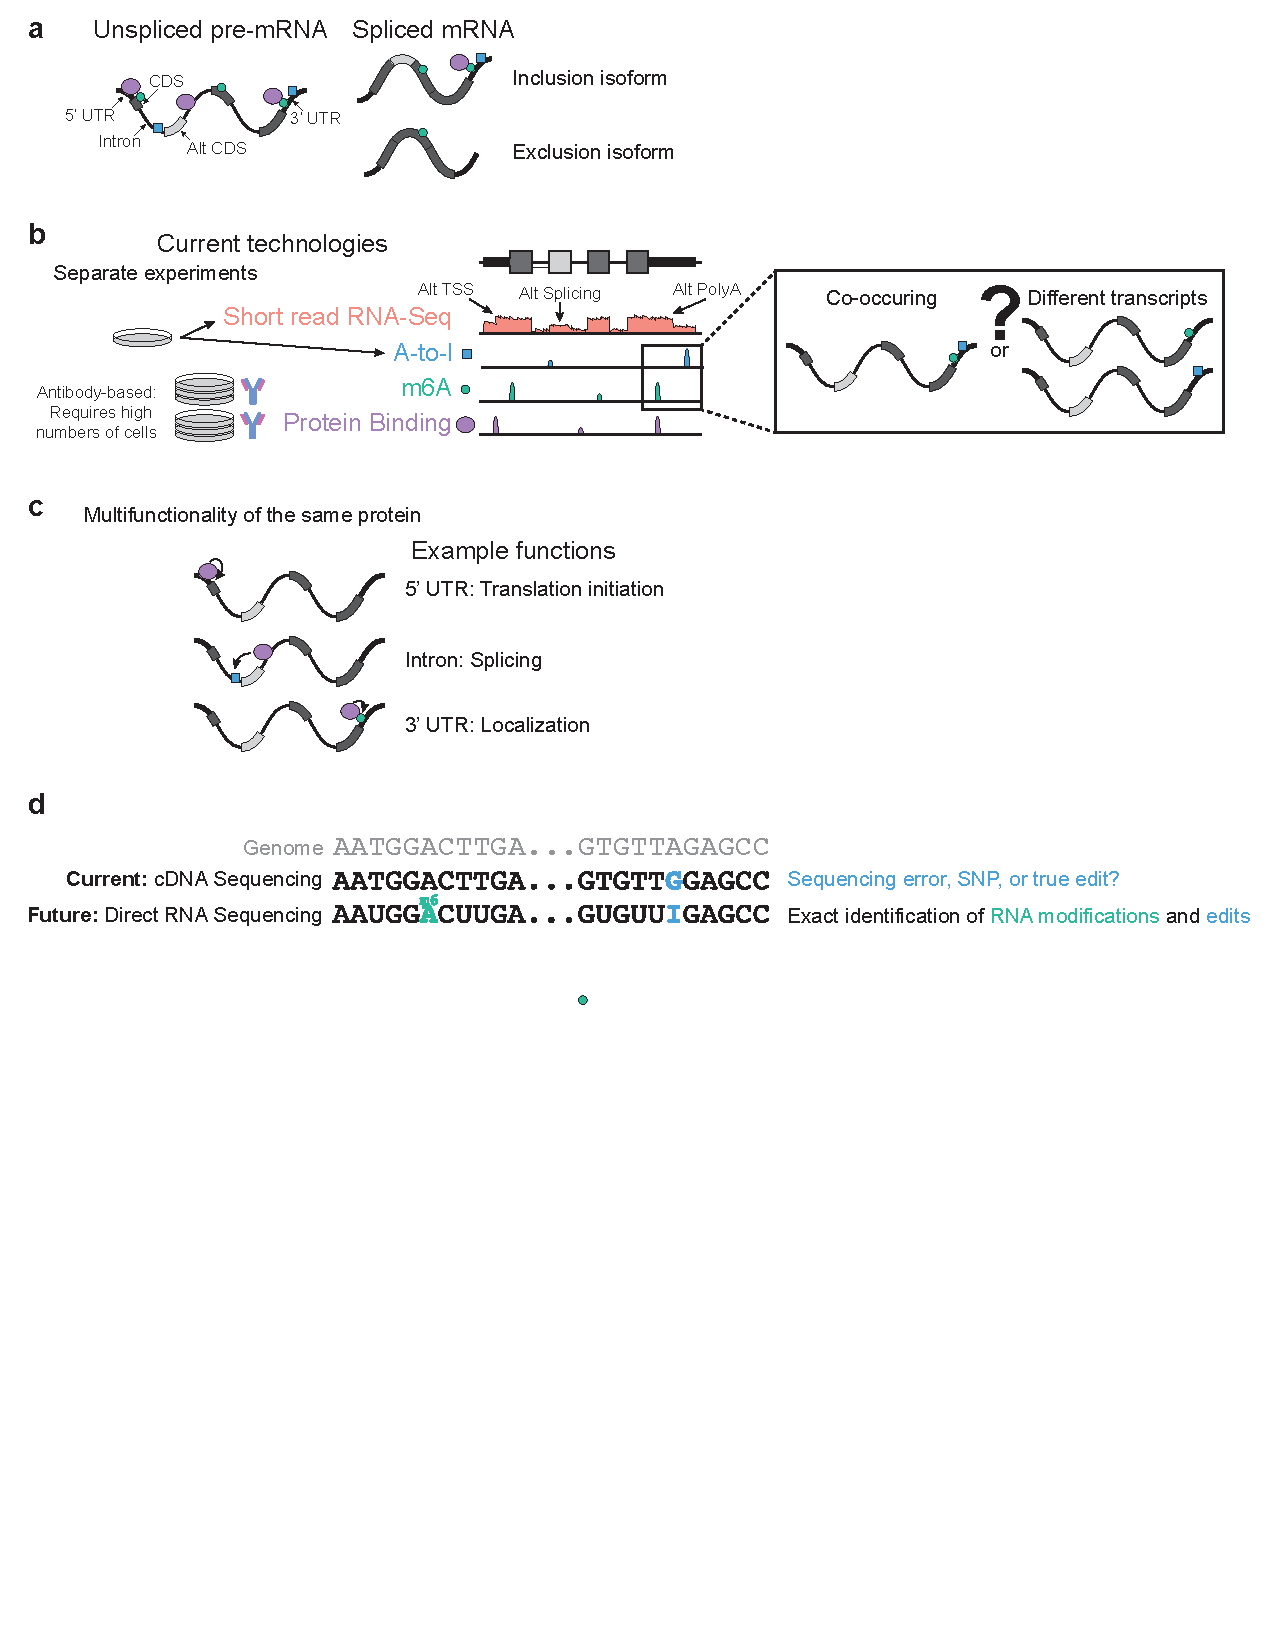
\includegraphics[width=5.8in]{figures/singlecell_future_methods}
  \caption[Unmet needs in RNA processing and potential future technologies.]{Unmet needs in RNA processing and potential future technologies.\\
\textbf{a.}~Left, example RNA transcript with RBPs (purple), A-to-I editing (blue), and m6A (green). Right,  possible inclusion and exclusion isoforms with different post-transcriptional modifications of splicing, m6A, RBP binding, and m6A modification.\\
\textbf{b.}~Current technologies allow for visualization of RNA abundance, A-to-I editing, m6A methylation, and protein binding, but cannot determine whether these occur on physically different or the same molecules.\\
\textbf{c.}~Technologies are needed to investigate multifunctionality of the same protein, e.g. if it performs different functions based on where it binds in the transcripts. Additionally, this would be interesting to study redundancy of different proteins such as splicing factors.\\
\textbf{d.}~Future direct RNA sequencing technologies would allow for direct identification of multiple RNA modifications and edits on the same transcript, unlike currently available technologies.}
\label{fig:singlecell_future_methods}
\end{figure}


Previously, it was thought that there are certain ``uncertainty principles'' in biology, such that one could not know both both the genotype and phenotype of a living cell (Strippoli et al., 2005) or both the cellular ``position'' (current cell state) and ``momentum'' (a cell's past or future, i.e. its lineage or differentiation trajectories) (Shapiro et al., 2013). However, recent work has turned these principles on their head. Both the genotype and phenotype can be measured from a single cell by capturing both DNA and RNA (Macaulay et al., 2015; Reuter et al., 2016), even coupling with measuring DNA methylation and RNA (Angermueller et al., 2016; Hou et al., 2016). A cell's ``position'' and ``momentum'' can be inferred through algorithms that delineate cellular trajectories from phenotypic measurements such as RNA-seq, reviewed thoroughly by (Cannoodt et al., 2016). We expect more technologies to upend traditional thinking of what is possible at the single cell level.

\subsection{Co-occurrence and mutual exclusivity of RNA processing events}

Current technologies to measure transcript abundance and nucleotide modifications, must be performed in separate, bulk experiments, and beyond correlations, the co-occurrence of these [interactions] on the same transcript is unknown (Figure~\ref{fig:singlecell_future_methods}b). Future understanding of the interdependence of RNA processing will require the measurement of multiple aspects of RNA processing at once. This will require is direct RNA sequencing without creation of a cDNA template such as by the Oxford Nanopore MinION (Wanunu et al., 2011) or Pacific Biosciences Single Molecule Real-Time (SMRT) Sequencing (Flusberg et al., 2010). These technologies can directly detect RNA modifications such as m6A and inosine as presence of A-to-I editing (Carr, 2016; Garalde et al., 2016; Saletore et al., 2012). Unfortunately, these technologies are plagued with high error rates and this challenging problem of accuracy for single molecule sequencing will need to be addressed. Nonetheless, as the entire transcript is measured, these would also reveal the co-occurrence on relationships such as between alternative splicing and nucleotide modifications, shedding light on the co-dependence (or independence) of RNA processing elements.
Beyond measuring presence or absence of RNA and its modifications, the interactions of an RNA modification with structure and binding partners will be important. Current methods for measuring RNA secondary structure, typically by selectively measuring only single- or double-stranded RNA, require thousands of cells as input (Bevilacqua et al., 2016; Rouskin et al., 2014; Wan et al., 2011, 2014), thus averaging out the signal across many cells. Scaling these protocols down to single cells will be challenging, it will require tiny amounts of each reaction occurring in nanoliter volumes of captured cells.

\subsection{Spatial analysis: Tissue- and organ-level in vivo}

Disease focus (from Fernando)
ALS
To study ALS, People either extract the entire spinal cord or laser-capture microdissected motor neurons from the spinal cord
Nobody knows what the other cell types do 
How are the supporting glia, astrocytes affected in the ALS spinal cords?
Alzheimer's (from Alex Shishkin)
Market size is Billions of dollars
Hematopoiesis (from Fred)
Niches in the body
Responding to immune insults or lesions
Spatial mapping of the cell of origin with the RNA seq
Spatial mapping of gene expression back to 3d position of cells (Achim et al., 2015; Mori et al., 2017)
Ed boyden's methods
Spatial transcriptomics (Ståhl et al., 2016; Vickovic, 2017) 
Fixed tissue, barcode each location
Then do sequencing and reconstruct
Long Cai's methods (Frieda et al., 2017; Shah et al., 2016a)
Seurat (Satija et al., 2015)
Used known landmark genes
E.g. for a tumor, shave away the outer layer of cells, sequence, and keep going
How are genes differentially expressed?
Outer layer -- more prone to metastasis
Inner layer -- hypoxic

\subsection{Dynamics/time scale}

Most single-cell technologies are destructive -- once you sample the cell, you can't put it back and see how it responds in a new situation
``Single-cell uncertainty principle'' - similar to the ``uncertainty principle'' of measuring genetics in a living cell (Strippoli et al., 2005)
Originally defined for not knowing both the genotype and the phenotype of a living cell
In cellulo labeling of RNA (Custer and Walter, 2016)
Labels RNA fluorescently without adding much molecular weight


\subsection{Moonshot: Spatial + Dynamics}

Moon shot target: live cell imaging
Temporal dynamics could be measured by tracking RNA molecules with RNA-targeted CRISPR/Cas9 (Nelles et al., 2016), provided the technique scaled to the single molecule level.
Biggest problem: signal amplification

Watch assembly of the spliceosome in nuclear speckles in real time
Watch XIST crawl across the X-chromosome in real time
Step 1: live-cell abundance of one RNA
Cas9 + fluorophore
Step 2: Live-cell imaging of multiple RNAs
Cas9 + multiple fluorophores across several RNAs
Step 3: live-cell imaging of different ends of one RNA
Cas9 + multiple fluorophores at beginning, middle and end of the RNA



\subsection{Single cell multi-omics: One cell, many measurements}

A major problem in the field of high-throughput biology is that as soon as a facet of a molecule is digitized, all other context is lost. For example, measuring RNA may inhibit measuring DNA, and measuring RNA abundance cannot currently be performed simultaneously with investigation of nucleotide modifications. How can cellular context be maximized in a high-throughput manner?
This is a problem because the interplay between genotype and phenotype is lost.

One solution to ameliorate the lost context is simultaneous measurements of multiple categories of molecules. While simultaneous capture of the (epi-)genome and transcriptome have been major breakthroughs (Angermueller et al., 2016; Dey et al., 2015; Hou et al., 2016; Macaulay et al., 2015; Reuter et al., 2016), there are many more aspects of cellular state that are still invisible to the sequencing eye. 
Effect of non-RNA on RNA processing - e.g. DNA (chromatin, structure, SNPs) on RNA Processing (quantitative trait loci - QTLs)
Chromatin modifications and their effect on transcription speed and alternative splicing
Quantitative trait loci - SNPs + RNA processing
For example, abundances of proteins or metabolites in conjunction with RNA would provide a fuller picture of cellular state.
E.g. does presence of certain sugars or signaling molecules co-occur with certain RNAs? Discovery of novel signaling pathways
Chromatin structure, along time 4D nucleome (Dekker et al., 2017)
Post-translational modifications of proteins (phosphorylation, glycosylation)
RBPs are glycosylated
Does an RBP bind different regions, perform different functions, or interact with different proteins, when it is differentially glycosylated?
Time scale: phosphorylation can be on the order of seconds

Another method to create additional context for each individual cell is to combine high-throughput measurements with genome editing such as with CRISPR/Cas9, allowing for dissection of complex phenotypes in mammalian cells at large scales. For example, Perturb-seq is a method that combines knockdown of genes using CRISRPi with single-cell RNA-seq, and was used to study the unfolded protein response (Adamson et al., 2016) and effect of lipopolysaccharides on dendritic cells (Dixit et al., 2016). This created a computational scientist's dream dataset, as for each gene that was knocked down, there was a control dataset, and thus for developing algorithms, one could always have a negative control to check with. Perturb-Seq could be applied to study any aspect of RNA processing, e.g. systematically knocking down all protein components of the spliceosome or different alternative splicing factors. 
Another possibility is coupling RNA-seq with lineage-specific barcodes through genome editing by CRISPR/Cas9 (McKenna et al., 2016). This would allow for comparing the transcriptomes of cells from similar lineages. Using phylogenetic techniques, cell lineages could be reconstructed and even the times at which cells asymmetrically divided to change fates could be found. If RNA-seq encodes a cell's present, then its traced lineage encodes its past. This lineage tracing method, coupled with direct RNA sequencing, would help to understand how developmentally regulated RNA processing events such as RNA editing, m6A, and alternative splicing, are finely tuned in different lineages. Do all cells that were committed to a particular lineage also have certain RNA processing events? This could indicate inheritability of the event, either encoded through the genome or by asymmetrically dividing the RNA content of a mother cell.


\section{Discussion}

Previous ‘single-cell' studies were limited to microscopy and other visual tools
Ultimately, ‘single-cell biology' is ‘biology'
Each RNA lives a rich, fulfilled life, and this is difficult to measure through single-cell techniques due to technical limitations.
Many questions remain
How do the many transient aspects of RNA, such as nucleotide modifications, binding partners, 3D structure, and localization, affect each other?
So far has been studied for one transcript, a few modifications
May not even know to study the co-interaction between these aspects on a particular transcript

\chapter{The \emph{Expedition} software suite: Computational tools for transcriptome analysis}


% From main text: We developed Expedition, a suite of algorithms integrated in a complete software package designed to address three key concepts that are critical for single-cell analyses: (1) rejection of an alternative event if its definition is incompatible with the data, and (2) ability to describe the variation of AS such as detect bimodality and (3) visualize AS distribution changes from one cell type or state to another.

In this paper, we developed the \emph{Expedition} suite, consisting of  software packages that addressed three key deficiencies in single-cell alternative splicing analysis:

\begin{enumerate}
	\item \textbf{Detect and quantify alternative splicing quickly, with minimum false positives: \outrigger, \Cref{sec:outrigger}}\\
	In single-cell analysis, absolute quantitation of gene expression or ``percent spliced-in'' (Psi/$\Psi$) is important and enable us to learn the distribution of these quantitations. Previously, relative quantitation for splicing ($\Delta\Psi$) is more commonly used to calculate the difference between groups. Such relative quantitation tolerates false positive better, as false positives may not vary between groups, $\Delta\Psi \sim 0$ and are thus not noticeable in pairwise comparisons. However, when studying distribution of absolute quantitation, such false positives obscure the observation in unpredictable way and hinder biological interpretation. The second main problem of previous splicing algorithm is the inflexible definitions of alternative exons. The same alternative exons may utilize different flanking exons in different cells/samples, thus leading to different biological interpretation. To address these problems, we create \outrigger, which uses junction reads to find de novo exons, creates a splice graph to define junction-based alternative events, filters for conserved splice sites, and strictly rejectes cases of alternative events incompatible with the data at hand. Finally, we discuss and compare to the popular MISO\cite{Katz:2010iv} algorithm.
	\item \textbf{Classify modalities of alternative splicing events, including bimodal: \anchor, \Cref{sec:anchor}}\\
	The power of single-cell analyses rises from the ability to study the distribution of a parameter-of-interest. There are a few statistical methods for finding bimodal distributions, but none are sufficient because they are either not sensitive enough, or not robust enough to noise. Additionally, these methods only deal with bimodal distribution and do not classify other distributions, such as unimodal or multimodal. To create a sensitive distribution classifier for all modalities, we used Bayesian methods to create \anchor, and compare our method to a simple binning method, the bimodality index\cite{Wang:2009wm}, and the bimodal dip test\cite{Hartigan:1985ca}.
	\item \textbf{Quantify and visualize dynamics in distributions: \bonvoyage,\linebreak \Cref{sec:bonvoyage}}\\
	While there are many statistical tests to compare changes in distributions, few of them is coupled with visual tools to present changes in distribution with both magnitude and direction. For the specific question of alternative splicing changes, we are interested in observing a event becomes more included or more excluded. Thus we have employed machine learning methods to create a visualizable, interpretable 2d space with ``included'' and ``excluded'' axes. This method is compared to the quantification offered by the Jensen-Shannon Divergence (JSD)\cite{Cover:2011vn}.
\end{enumerate}

\section{\texttt{outrigger}: Splicing estimation with \emph{de novo} annotation and graph traversal}
\label{sec:outrigger}

Currently available tools for AS detection and quanitification have two major problems: (1) inflexible definitions that cannot handle different configurations of flanking exons for the same alternative junctions, and (2) lack of rejection of an alternative event even if its definition is incompatible with the data-at-hand. The first problem is solved with \texttt{outrigger index}, which defines all potential alternative events based on the junctions and alternative exons from the aggregate of entire sample sets in a given project, and enumerates all biologically possible flanking exon combinations. This step maximize the likelihood to identify all possible alternative events. To ensure only valid alternative events were generated, we added \texttt{outrigger validate} to remove alternative events with introns lacking conserved splice sites. The second prolbem is solved with \texttt{outrigger psi}, which applies strict rules to only permit junctions with sufficient coverage for an event in a given sample. All the parameters in the rules can be user-defined. Thus, outrigger addresses key issues with current alternative splicing software.

\subsection{Algorithm overview}

Broadly, the goal of \outrigger\, is to create a custom, \emph{de novo} alternative splicing annotation by using junction reads and exon definitions to create a exon-junction graph, traversing the graph to find alternative events, and calculate percent spliced-in (Psi/$\Psi$) of the alternative exons.


\begin{figure}[h]
  \centering
  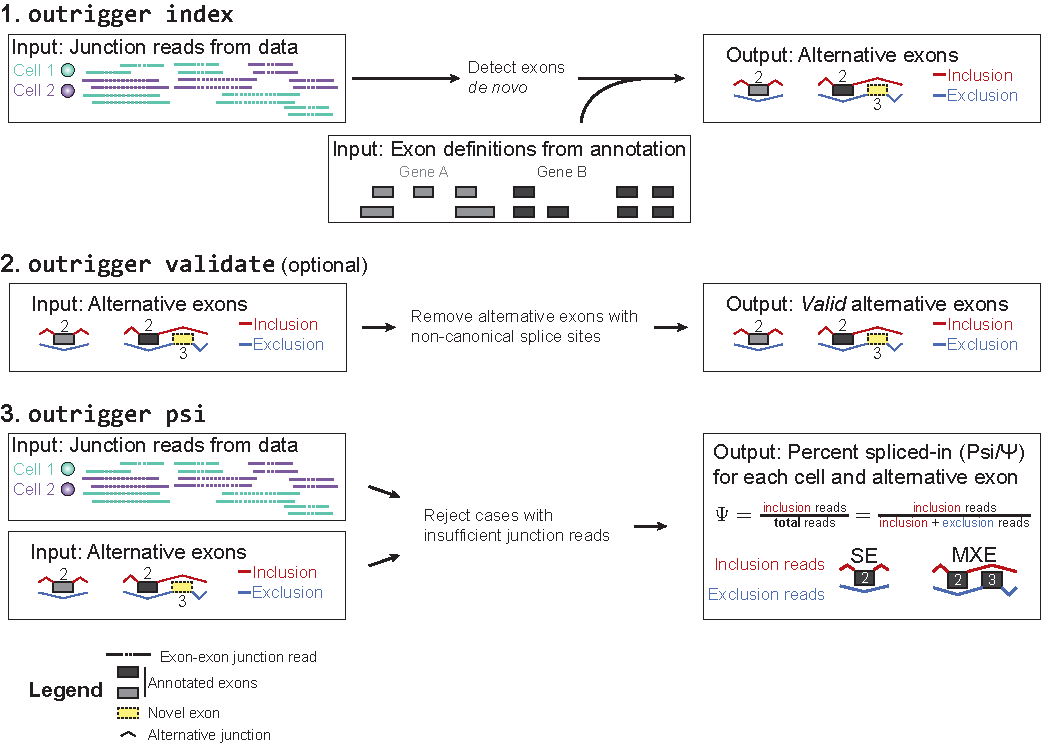
\includegraphics[width=5.6in]{figures/outrigger_overview.pdf}
  \caption[Overview of \outrigger's three steps and associated commands: indexing (\texttt{outrigger index}), validation (\texttt{outrigger validate}) and percent spliced-in (Psi/$\Psi$) calculation (\texttt{outrigger psi})]{Overview of \outrigger's three steps and associated commands: indexing (\texttt{outrigger index}), validation (\texttt{outrigger validate}) and percent spliced-in (Psi/$\Psi$) calculation (\texttt{outrigger psi}). In the first step of building an index, \outrigger\, considers the entirety of junction reads from the user-input dataset to detect exons \emph{de novo}, adds annotated exons, then searches for alternative exons. In the second, optional, step of validating the detected events, \outrigger\, removes alternative exons with flanking introns lacking consensus splice sites. For the third step of calculating Psi/$\Psi$, \outrigger\, utilizes junction reads together with alternative exons defined in the indexing step and calculates $\Psi$ for each sufficiently covered event. Only junction reads are used to represent inclusion or exclusion reads. SE, Skipped Exon; MXE, Mutually Exclusive Exons.
  }
  \label{fig:outrigger_overview}
\end{figure}




% --- BEGIN manual facingcaption --- %
\clearpage
\thispagestyle{facingcaption}
\begin{figure}[h]
\captionsetup{labelformat=prev-page}
  \caption[Internal steps of indexing via \texttt{outrigger index}: Exons identification and defining alternative events.]{
  Internal steps of indexing via \texttt{outrigger index}: Exons identification and defining alternative events.\\
% \captionof{figure}{\textbf{} \\
\textbf{a.} Internal workings of the indexing step via \texttt{outrigger index}. User-provided inputs junction reads can be either genome-aligned \texttt{.bam} files, the \texttt{.SJ.out.tab} splice junction files from the STAR aligner, or a compiled table in \texttt{.csv} of all junction reads from all samples for the project. Step 1, only junction reads with sufficient depth in a cell/sample are retained. By default, the minimum number of reads is $10$ per cell/sample, which can be modified with the flag \texttt{-{}-min-reads}. Step 2, junction reads are used to identify junction locations, and reads are aggregated across all cells/samples regardless of which cell/sample it came from. Step 3, if there is a ``gap'' between two junctions that is smaller than certain length $X$ (by default, $X=100$ nucleotides but can be modified with the flag \texttt{-{}-max-de-novo-exon-length}), then an exon is inserted. Step 4, the identified exons are compared with the annotated exons to obtain the pairwise relationships between exons and junctions. Step 4 outputs a table of ``triples:'' of \texttt{(exon, direction, junction)} encoding the directional relationship between exons and junctions. Step 5, the output tables from step 4 are utilized to connect exons through junctions and creates a graph database. Finally, in Step 6, alternative exons are identified by traversing the graph database. The output of the indexing step run by the command \texttt{outrigger index}, is junction-based, outputting the alternative exon and all possible configurations of flanking exons for each event. For example, on the bottom right, the same skipped exon event using the same alternative junctions, have four possible configurations of flanking exons. They are considered to be the same event, but are reported with all four configurations for the ease-to-use in downstream analysis.\\
\textbf{b.} Defining alternative events and comparison of biological interpretability of events found by MISO and \outrigger. For a given alternative exon (black box), there can be multiple transcripts corresponding to the alternative exon but with different flanking exons. MISO chooses to define the alternative event using the shortest exons on both sides. Yet, this MISO-defined alternative event may not actually exist as a transcript in the dataset and will be misleading to interpret. For example, attempts to translate such non-existing transcript(s) will be inappropriate. In contrast, \outrigger\, defines the event based on the junctions, and outputs all corresponding flanking exon configurations, thus enabling broader use of the outputs and more relevant biological interpretation.
}
\label{fig:outrigger_index}
\end{figure}
\clearpage
\begin{figure}[h]
\ContinuedFloat
\captionsetup{labelformat=empty}
\centering
% \includegraphics[width=5.8in]{sandiego.jpg}
  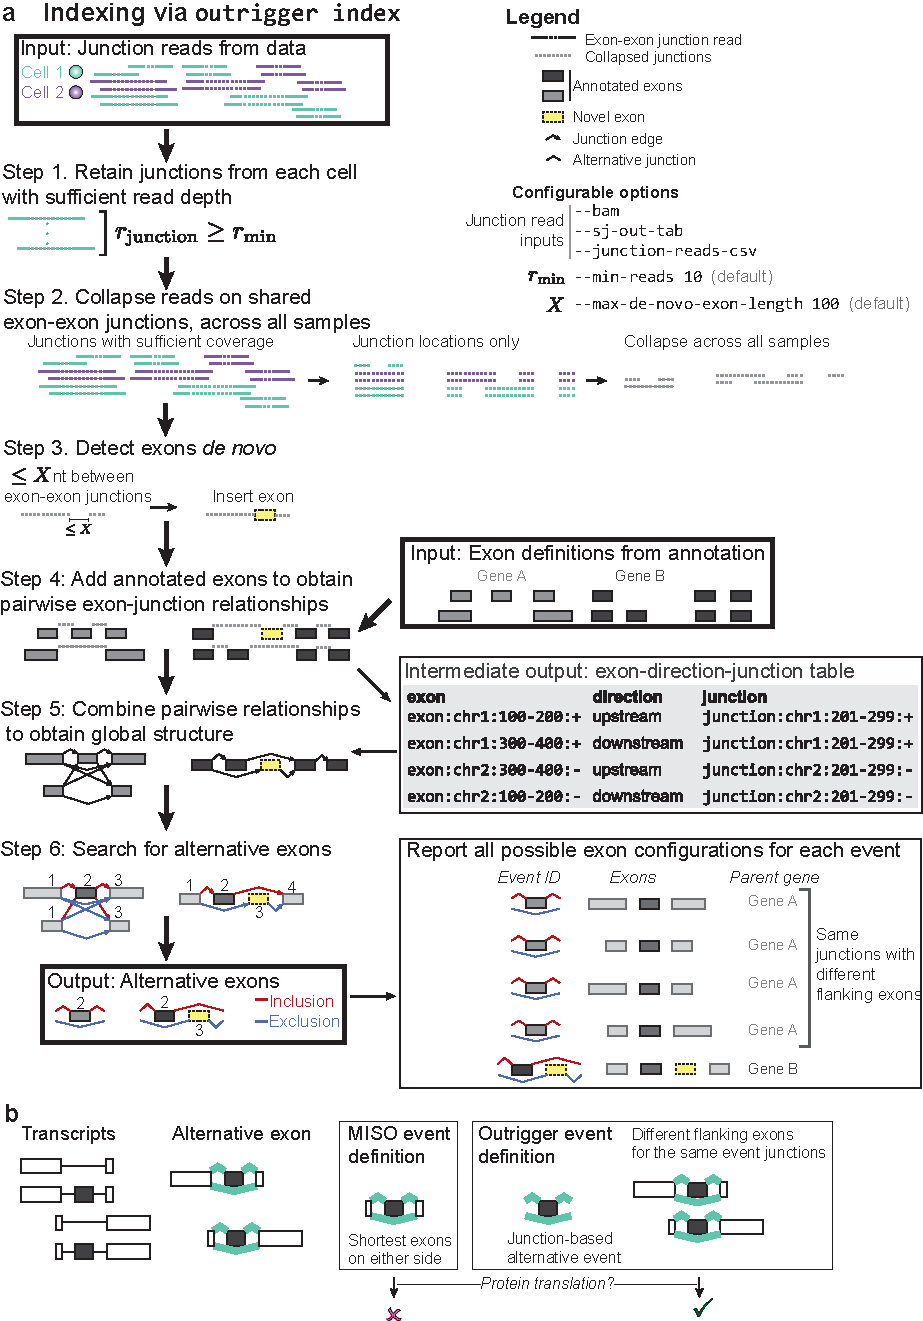
\includegraphics[width=5.8in]{figures/outrigger_index}
\end{figure}
%and, I'm not sure why, but one of the times I used this code the figure number wasn't augmented for the next figure, so check your figure numbers and if necessary uncomment the following line
\addtocounter{figure}{1}
\clearpage
% --- END manual facingcaption --- %


\paragraph{\texttt{outrigger index}: Create custom alternative splicing annotation.} The following is a narrative describing \textbf{\Cref{fig:outrigger_index}a}.


\subparagraph{Inputs.} Two inputs are required for \texttt{outrigger index}: junction counts and gene annotations. The junction counts can be provided in many forms: either \texttt{.bam} \cite{Group:OEYDIUUE} genome alignment files, splice junction count \texttt{.SJ.out.tab} files created by the STAR aligner\cite{Dobin:2013fg}, or a pre-compiled table of samples' junction reads in a \texttt{.csv} format. The gene annotations can be provided in \texttt{.gtf} or \texttt{.gff} format.

\subparagraph{Step 1: Retain junctions from each cell with sufficient read depth.} Junctions with reads in an individual sample less than the minimum number of reads, $r_{\min}$ are removed. By default, $r_{\min} = 10$, and can be adjusted by the user, for example to a minimum of 88 reads, with \texttt{-{}-min-reads~88} on the command line. To illustrate, if one junction is observed with two (2) reads in 100 samples, although there were a total of 200 reads observed on the junction, it will be discarded at this step. Because, there is not sufficient evidence to suggest that this junction is well-covered in any sample.

\subparagraph{Step 2: Collapse reads on shared exon-exon junctions, across all samples.} The aggregate of all junctions from all samples in a given project are create to maximize the likelihood of identifing all potential alternative events.

\subparagraph{Step 3: Detect exons \emph{de novo}.} If the gap between two junctions is under $X$ nucleotides, an exon will be inserted at the gap. This maximum $X$ is necessary, because otherwise we could insert ``exons'' that are many kilobases long, but aren't true exons -{}- they are the intergeneic space between genes. By default, $X = 100$, and this can be adjusted by the user, for example to 157 nucleotides, with the command line flag, \texttt{-{}-max-de-novo-exon-length~157}.

\subparagraph{Step 4: Integrate exon annotation to obtain pairwise exon-junction relationships.} Annotated exons are integrated with the \emph{de novo} exons and create a table of the pairwise relationships of each exon to each junction. We do this by creating a database of genes, transcripts, and exons from a GTF gene annotation file using \texttt{gffutils} \cite{gffutils:sP8uhXuv}, and observing which junctions are adjacent to each exon. This outputs an \emph{``exon-direction-junction''} table which is used in Step 5.

\subparagraph{Step 5: Combine pairwise relationships to obtain global structure.} We then use the adjacencies to build a directional graph which connects exons to each other via junctions. This graph database was built using \texttt{graphlite} \cite{graphlite:vt}, a Python program that provides a lightweight graph wrapper over SQLite.

\subparagraph{Step 6: Search for alternative exons.} To find alternative events, all exons in the graph database were transversed to test, if starting from that exon, it could be a first exon of an skipped exon (SE) or mutually exclusive exon (MXE) event.

\subparagraph{Outputs.} The output of \texttt{outrigger index} is a folder containing the following. The \texttt{events.csv} file contains the event definitions will be used by \texttt{outrigger psi}. The \texttt{exonN.bed} files, where \texttt{N} is an exon number, will be used by \texttt{outrigger validate} to check for canonical or non-canonical splice sites.

The splicing event definitions in the \texttt{events.csv} files are specified by the junctions and the alternative exon. As there may be multiple potential flanking exons with the same junctions, rather than choosing a single version (as is done by MISO, \textbf{\Cref{fig:outrigger_index}b}), we output all possible flanking exon configurations. Thus, while the critical alternative exons are exon 2 for SE events and exons 2 and 3 for MXE events, we show all possible exon flanking exon 1s and exon 3s for SE, and all possible flanking exon 1s and exon 4s for MXE events (\textbf{\Cref{fig:outrigger_index}a}, lower right).

Below is an example command using \texttt{outrigger index}:

\begin{verbatim}
outrigger index --bam *sorted.bam \
    --gtf gencode.vM10.annotation.gtf
\end{verbatim}

This creates a folder called \texttt{outrigger\_output} with the following contents:


\begin{figure}
\footnotesize
\dirtree{%
.1 outrigger\_output/.
.2 index.
.3 gtf\DTcomment{Added by Step 3}.
.4 gencode.vM10.annotation.gtf\DTcomment{Added by Step 4}.
.4 gencode.vM10.annotation.gtf.db\DTcomment{Added by Step 4}.
.4 novel\_exons.gtf\DTcomment{Added by Step 3}.
.3 exon\_direction\_junction.csv\DTcomment{Added by Step 4}.
.3 mxe\DTcomment{Added by Step 6}.
.4 event.bed\DTcomment{Added by Step 6}.
.4 events.csv\DTcomment{Added by Step 6}.
.4 exon1.bed\DTcomment{Added by Step 6}.
.4 exon2.bed\DTcomment{Added by Step 6}.
.4 exon3.bed\DTcomment{Added by Step 6}.
.4 exon4.bed\DTcomment{Added by Step 6}.
.4 intron.bed\DTcomment{Added by Step 6}.
.3 se\DTcomment{Added by Step 6}.
.4 event.bed\DTcomment{Added by Step 6}.
.4 events.csv\DTcomment{Added by Step 6}.
.4 exon1.bed\DTcomment{Added by Step 6}.
.4 exon2.bed\DTcomment{Added by Step 6}.
.4 exon3.bed\DTcomment{Added by Step 6}.
.4 intron.bed\DTcomment{Added by Step 6}.
.2 junctions\DTcomment{Added by Step 1}.
.3 metadata.csv\DTcomment{Added by Step 2}.
.3 reads.csv\DTcomment{Added by Step 1}.
}
\caption{Example output of \texttt{outrigger index} command.}
\end{figure}


Besides outputting the relevant \texttt{events.csv} which is used in \texttt{outrigger psi} to define events, we also output \texttt{.bed} files for the entire event, the alternative intron, and each exon, facilitating downstream sequence analysis.


\paragraph{\texttt{outrigger validate}: Remove alterantive splicing lacking conserved splice sites.} The following describes the biological intuition behind \textbf{\Cref{fig:outrigger_validate_frankenevents}a}. Major (U2) splicesome recognize splice-sites as  ($5^\prime$ end of intron/$3^\prime$ end of intron) \texttt{GT/AG} and \texttt{GC/AG} the Minor (U12) spliceosome recognizes splice-sites as \texttt{AT/AC}\cite{McManus:2011en,GarciaBlanco:2004kl}. By default, these combinations of splice-sties are allowed. But the valid splice sites can be user-specified and changed for example to \texttt{AA/AA} and \texttt{GG/GG} with \texttt{-{}-valid-splice-sites~AA/AA,GG/GG}.

The output of \texttt{outrigger validate} is a \texttt{splice\_sites.csv} folder containing the splice sites, and an additional folder in the splice type folder, called \texttt{validated}, containing filtered \texttt{events.csv} which only contain alternative events with valid splice sites. For example, as a follow up on our previous \texttt{outrigger index} command, we validate the alternative exons with the command,

\begin{verbatim}
outrigger validate -{}-genome mm10 \
    -{}-fasta GRCm38.primary_assembly.genome.fa
\end{verbatim}

This creates the following additions to the \texttt{outrigger\_output} folder:

\begin{figure}
\footnotesize
\dirtree{%
.1 outrigger\_output/.
.2 index.
.3 gtf.
.4 gencode.vM10.annotation.gtf.
.4 gencode.vM10.annotation.gtf.db.
.4 novel\_exons.gtf.
.3 exon\_direction\_junction.csv.
.3 mxe.
.4 event.bed.
.4 events.csv.
.4 exon1.bed.
.4 exon2.bed.
.4 exon3.bed.
.4 exon4.bed.
.4 intron.bed.
.4 splice\_sites.csv\DTcomment{Added by \texttt{outrigger validate}}.
.4 validated\DTcomment{Added by \texttt{outrigger validate}}.
.5 events.csv\DTcomment{Added by \texttt{outrigger validate}}.
.3 se.
.4 event.bed.
.4 events.csv.
.4 exon1.bed.
.4 exon2.bed.
.4 exon3.bed.
.4 intron.bed.
.4 splice\_sites.csv\DTcomment{Added by \texttt{outrigger validate}}.
.4 validated\DTcomment{Added by \texttt{outrigger validate}}.
.5 events.csv\DTcomment{Added by \texttt{outrigger validate}}.
.2 junctions.
.3 metadata.csv.
.3 reads.csv.
}
\caption{Example output of \texttt{outrigger validate} command.}
\end{figure}


\paragraph{Potential ``Franken-events'' created by combining junctions over multiple datasets.} As many junctions may occur spuriously in a single cell (sample), aggregating all junctions across all cells (sample) may create events that were not observed in any individual cell (\Cref{fig:outrigger_validate_frankenevents}b). We wanted to ensure we strictly defined when events were valid or not in these cases.

In the case of SE events, the exon will have $\Psi = \text{NA}$ for the cell with the observed inclusion junctions, since they don't have sufficient reads on both sides of the exon. For the cell with the exclusion junction, it will have $\Psi = 0$ since no inclusion reads were observed.

For MXE events, if each of the four junctions was observed independently in a different cell, then all of the cells will have $\Psi = \text{NA}$ for that splicing event since there are no cells which have sufficient reads on all junctions of either isoform.

\begin{figure}
  \centering
  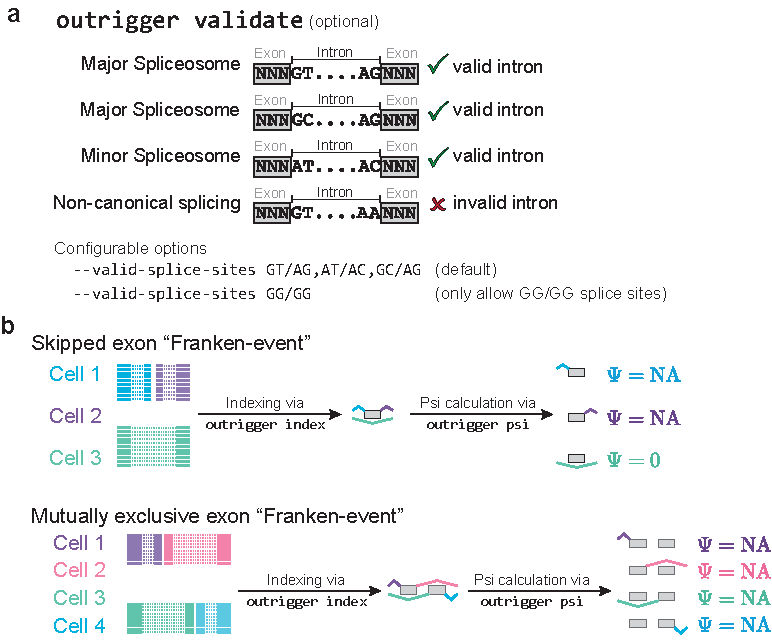
\includegraphics[width=5.8in]{figures/outrigger_validate}
  \caption[\outrigger\, validation and pathological cases.]{
  \outrigger\, validation and pathological cases.\\
\textbf{a.}~Validation via \texttt{outrigger validate}: Removal of alternative events with introns lacking consensus splice sites. In this optional step, exons with flanking introns lacking known splice site motifs are removed. This is configurable. By default, the valid splice sites are specified as, \texttt{-{}-valid-splice-sites GT/AG,GC/AG,AT/AC}, but can be any pair of two nucleotides.\\
\textbf{b.}~Possible pathological cases of \texttt{outrigger}. These ``Franken-events'' consist of junctions that were observed in independent samples. At the indexing step, aggregated reads from multiple cells/samples are considered to construct an index of all junctions to maximize the number of AS events. Yet, at the Psi/$\Psi$ calculation step, in each individual cell/sample, insufficient reads may be observed for certain junction resulting in $\Psi=\text{NA}$ in some cells/samples for the same event. Top, skipped exons, if each junction is observed only in one cell, the cell with the exclusion junction is assigned a $\Psi=0$ while the remaining cells are assigned as $\Psi=\text{NA}$. Bottom, mutually exclusive exons, $\Psi=\text{NA}$ for all 4 cells, as there is insufficient evidence of exon inclusion or exclusion in any one cell. Thus, the number of detected events output by \texttt{outrigger index} can greatly overestimate the number of valid events in the dataset found by \texttt{outrigger psi}.
}
\label{fig:outrigger_validate_frankenevents}
\end{figure}



\paragraph{\texttt{outrigger psi}: Calculate percent spliced-in of alternative exons}

To calculate percent spliced-in (Psi/$\Psi$) of a potentially alternative exon identified in \texttt{outrigger index}, we use the equation for $\Psi= \frac{\text{inclusion reads}}{\text{total reads}}$ \cite{Wang2008-xh}, with substantial checks for whether the event is valid (\textbf{\Cref{fig:outrigger_psi}}). For SE, there is only one exclusion junction and thus the the exclusion junction is weighted by two to compensate (Eq.~\Cref{eq:se_psi}). For MXE, the calcluation is simply the inclusion reads divided by the total reads (Eq.~\Cref{eq:mxe_psi}). The junction reads between exon $i$ and exon $j$ are presented as $r_{i,j}$, displaying inclusion reads in red and exclusion reads in blue.

\begin{multicols}{2}
\noindent
  \begin{gather}
  \text{SE $\Psi$}\nonumber\\
\Psi = \frac{\textcolor{inclusion}{r_{1,2}} + \textcolor{inclusion}{r_{2,3}}}{\textcolor{inclusion}{r_{1,2}} + \textcolor{inclusion}{r_{2,3}} + 2\textcolor{exclusion}{r_{1,3}}} \label{eq:se_psi} %\nonumber
\end{gather}
% \break
\begin{gather}
  \text{MXE $\Psi$}\nonumber\\
\Psi = \frac{\textcolor{inclusion}{r_{1,2}} + \textcolor{inclusion}{r_{2,4}}}{\textcolor{inclusion}{r_{1,2}} + \textcolor{inclusion}{r_{2,4}} + \textcolor{exclusion}{r_{1,3}} + \textcolor{exclusion}{r_{3,4}}} \label{eq:mxe_psi} %\nonumber
\end{gather}
\end{multicols}

Multiple validation steps were incorporated to ensure that the junction reads observed in each sample are consistent with the type of splicing event annotated by \outrigger. This process is described in \textbf{Supplementary Software .~\Cref{fig:outrigger_psi}}.

% --- BEGIN manual facingcaption --- %
\clearpage
\thispagestyle{facingcaption}
\begin{figure}[h]
\captionsetup{labelformat=prev-page}
  \caption[Cases created by percent spliced-in calculation via the command \texttt{outrigger psi}.]{
  Cases created by percent spliced-in calculation via the command \texttt{outrigger psi}.\\
% \captionof{figure}{\textbf{}
The table describes the 11-step sequential logic of \outrigger\, to reject an event in a cell/sample based on that cell/sample's junction reads. If an event reaches a $\Psi=\text{NA}$ case, then it is rejected from that sample, otherwise, it continues through the cases. If the event is rejected, then it is assigned $\Psi = \text{NA}$, if it is not rejected, then it gets a $0\leq \Psi \leq 1$ value based on the junction reads.\\
Strict evaluation of percent spliced-in (Psi/$\Psi$). To compute the percent spliced-in (Psi/$\Psi$) of skipped exon (SE) and mutually exclusive exons (MXE) alternative events during the execution of the command \texttt{outrigger psi}, we use $\Psi= \frac{\text{inclusion reads}}{\text{total reads}}$. We represent the number of reads spanning the junction between exon$_i$ and exon$_j$ as $r_{i,j}$.
}
\label{fig:outrigger_psi}

\end{figure}
\clearpage
\begin{figure}[h]
\ContinuedFloat
\captionsetup{labelformat=empty}
\centering
% \includegraphics[width=5.8in]{sandiego.jpg}
  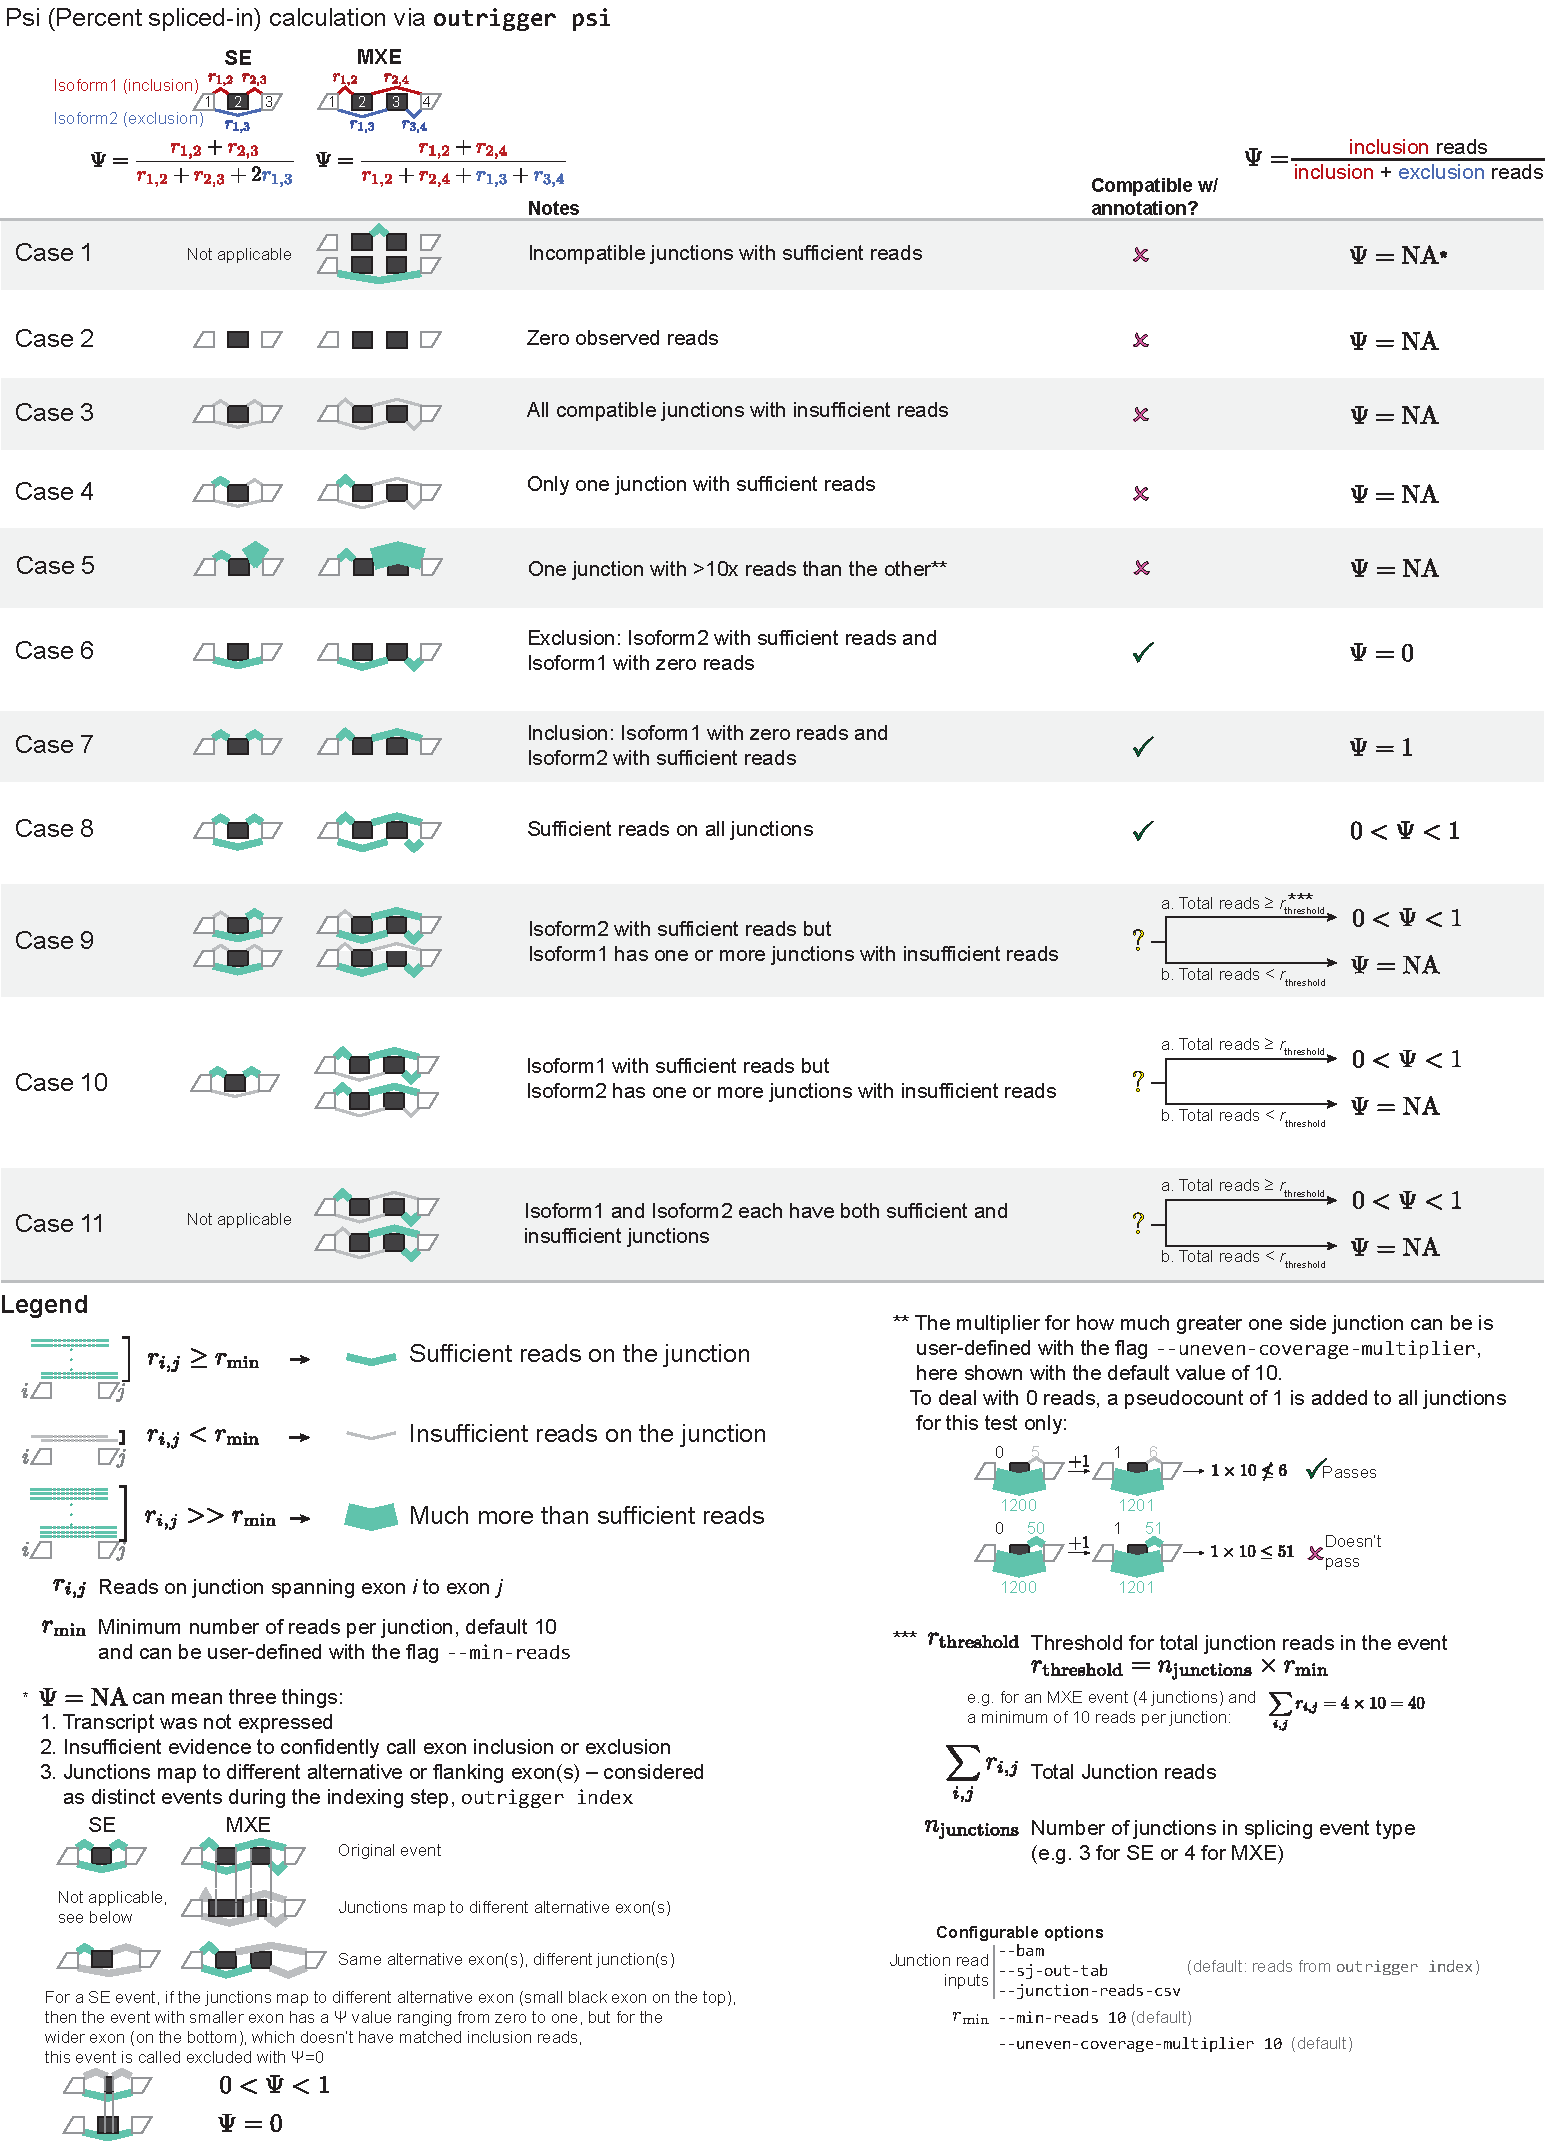
\includegraphics[width=5.8in]{figures/outrigger_psi}
\end{figure}
%and, I'm not sure why, but one of the times I used this code the figure number wasn't augmented for the next figure, so check your figure numbers and if necessary uncomment the following line
\addtocounter{figure}{1}
\clearpage
% --- END manual facingcaption --- %

\begin{longdescription}
	\item[Case 1: Incompatible junctions with sufficient reads.] This step checks whether the junction reads are compatible with a MXE event, or rather a twin cassette event. Specifically, evidence of  $r_{2,3} > r_{\min}$ or $r_{1,4} > r_{\min}$ suggests this junction is a twin cassette event but not an MXE event. In such cases, $\Psi = \text{NA}$. As described in \texttt{outrigger index}, the minimum number of reads is user-defined, for example to 37 with \texttt{-{}-min-reads~37}.
	\item[Case 2: Zero observed reads.] Given no reads is observed, this event is $\Psi = \text{NA}$, rather than $\Psi=0$ since $\Psi=0$ indicates exclusion.
	\item[Case 3: All compatible junctions with insufficient reads.] No single junction has the minimum number of reads $r_{\min}$, by default $r_{\min}$ is 10, and can be modifiable by the \texttt{-{}-min-reads} flag. If this is the case, we assign $\Psi = \text{NA}$.
	\item[Case 4: Only one junction with sufficient reads.] This applies to a single junction of two junctions per isoform, e.g. Isoform2 of either SE or MXE events, and Isoform1 of an MXE event, has sufficient reads. Since only one junction has the minimum number of reads, $r_{\min}$, no sufficient evidence indicates inclusion of exon-of-interest, thus, we assign $\Psi = \text{NA}$.
	\item[Case 5: One junction with $>10\times$ more reads than the other.] When the alternative exon is covered on the two sides with junction reads of great disparity, there is insufficient evidence supporting the inclusion of alternative exon or suggests the exon may involved in a complex splicing, rather than a SE or MXE. Thus, $\Psi = \text{NA}$. The default multiplier is 10 and can be modified by the user, for example to 55 by \texttt{-{}-uneven-coverage-multiplier~55}.
	\item[Case 6: Exclusion: Isoform2 with sufficient reads and Isoform1 with zero reads.] All junctions on Isoform2 have greater than the minimum reads $r_{\min}$, and all junctions of Isoform1 have no observed reads, thus $\Psi = 0$.
	\item[Case 7: Inclusion: Isoform2 with zero reads and Isoform1 with sufficient reads.] All junctions on Isoform2 have no observed reads and all junctions of Isoform1 have greater than the minimum reads $r_{\min}$, thus $\Psi = 1$.
	\item[Case 8: Sufficient reads on all junctions.] Both Isoform1 and Isoform2 have greater than the minimum reads on all their junctions. This is the best possible case for alternative splicing.
	\item[Case 9: Isoform2 with sufficient reads but Isoform1 has one or more junctions with insufficient reads.] If the exclusion isoform, Isoform2 has sufficient reads, but the inclusion isoform (Isoform1) does not, then we assess whether the total read coverage of the event, $\sum_{i,j} r_{i,j}$exceeds $r_{\text{threshold}}$. If so, a $\Psi$ is calculated; if not, $\Psi = \text{NA}$. We define $r_{\text{threshold}}$ as the number of junctions $n$ times the minimum number of reads $r_{\min}$. For example, with a minimum read count is 10 on an SE event, $r_{\text{threshold}} = 30$. For a minimum read count of 10 on an MXE event, $r_{\text{threshold}} = 40$.
	\item[Case 10: Isoform2 has one or more junctions with insufficient reads but Isoform1 has sufficient reads.] Similar to Case 9, we again test if the total read coverage is sufficient to calculate $\Psi$, i.e. if $\sum_{i,j} r_{i,j} \geq r_{\text{threshold}}$. If so, we calculate $\Psi$, and if not, we assign $\Psi = \text{NA}$.
	\item[Case 11: Isoform1 and Isoform2 each have both sufficient and insufficient junctions.] This case only applies to MXE events as SE events have as single Isoform2 junction, and cannot have both sufficient and insufficient junctions. If by the per-junction coverage, it is unclear whether the event has sufficient coverage, then we test if the total coverage of the event is sufficient. If so, we calculate $\Psi$, and if not, we assign $\Psi = \text{NA}$.
\end{longdescription}


% Before we calculate $\Psi$, we ensure that a sample has a valid SE event by checking for enough reads on either both the inclusion junctions ($r_{1,2}$ and $r_{2,3}$) or the exclusion junction ($r_{1,3}$). This protects against calculating $\Psi$ for events that aren't truly SE or MXE events, for example, an alternative first exon event that was annotated as an SE event would have $r_{1,2} = 0$, and thus we wouldn't calculate $\Psi$. For MXE events, we check that there are no reads between exons 2 and 3 ($r_{2,3}=0$), because if there are any reads here, then this is evidence that in a particular sample, this is a twin casette event rather than an MXE event (\textbf{Supplementary \Cref{fig:outrigger_psi}}). For SE events, we also check that for inclusion, there must be $>10$ reads on both sides of the alternative exon, and if there aren't, then we discard the event.
\subparagraph{Outputs} The output of \texttt{outrigger psi} is added into the \\\texttt{outrigger\_output} folder by creating a \texttt{psi} folder for each splice type. \texttt{psi.csv} contains $\Psi$ in a matrix, and the \texttt{summary.csv} produces a summary of all the events observed in all samples with their junction reads.

To follow up with our \texttt{outrigger index} and \texttt{outrigger validate} commands, we can run the below example command in the same directory:

\begin{verbatim}
outrigger psi
\end{verbatim}

This command adds to the existing output folder \texttt{outrigger\_output}. Therefore, we don't need to specify a genome location or reads or index location if this command is run from the same folder as the \texttt{outrigger index} command was run, and there exists in the directory a folder called \texttt{outrigger\_output}.

\begin{figure}
\footnotesize
\dirtree{%
.1 outrigger\_output/.
.2 index.
.3 gtf.
.4 gencode.vM10.annotation.gtf.
.4 gencode.vM10.annotation.gtf.db.
.4 novel\_exons.gtf.
.3 exon\_direction\_junction.csv.
.3 mxe.
.4 event.bed.
.4 events.csv.
.4 exon1.bed.
.4 exon2.bed.
.4 exon3.bed.
.4 exon4.bed.
.4 intron.bed.
.4 splice\_sites.csv.
.4 validated.
.5 events.csv.
.3 se.
.4 event.bed.
.4 events.csv.
.4 exon1.bed.
.4 exon2.bed.
.4 exon3.bed.
.4 intron.bed.
.4 splice\_sites.csv.
.4 validated.
.5 events.csv.
.2 junctions.
.3 metadata.csv.
.3 reads.csv.
.2 psi.\DTcomment{Added by \texttt{outrigger psi}}.
.3 mxe\DTcomment{Added by \texttt{outrigger psi}}.
.4 psi.csv\DTcomment{Added by \texttt{outrigger psi}}.
.4 summary.csv\DTcomment{Added by \texttt{outrigger psi}}.
.3 outrigger\_psi.csv\DTcomment{Added by \texttt{outrigger psi}}.
.3 se\DTcomment{Added by \texttt{outrigger psi}}.
.4 psi.csv\DTcomment{Added by \texttt{outrigger psi}}.
.4 summary.csv\DTcomment{Added by \texttt{outrigger psi}}.
}
\caption{Example output of \texttt{outrigger psi} command.}
\end{figure}

\paragraph{Advantages and limitations of \outrigger.}

The main advantages of \outrigger\, are speed and conserved memory footprint. As \outrigger\, operates only on junction reads, rather than resampling reads from a \texttt{.bam} alignment file, which can range in size from 500MB to 20GB and results in a high memory footprint, \texttt{outrigger} summarizes each \texttt{.bam} file to only its junction reads and uses that to estimate Psi/$\Psi$ values. Additionally, employing three steps of \outrigger\, \outrigger\ is able to maximize the number of potential alternative events and subsequently apply strict validation rules in the step of outrigger psi calculation to eliminate false positive events from each sample.
However, currently, \outrigger\ can only deal with SE and MXE events. We are in the process of incorporating other alternative splice types.

% \subsection{PCR duplicate removal studies}

% We also compared outrigger's performance on pre- and post-duplicate removed dataset. After duplicate-removal, ~93\% events were retained by requiring that each junction is covered by at least 10 unique reads (\textbf{Supplementary \Cref{fig:splicing_qc}f}). When comparing the Psi scores before and after duplicate-removal, the vast majority of events have a consistent Psi within |delta Psi| < 0.2 and only ~7\% are designated as NA in the latter (\textbf{Supplementary \Cref{fig:splicing_qc}h-i}), likely due to the reduced read coverage.

\subsection{Comparison to other methods}

In comparison to the popular splicing program MISO\cite{Katz:2010iv}, \outrigger\, has three major advantages:

\begin{enumerate}
	\item Ability to build de novo exon indexes (\texttt{outrigger index})
	\item Flexiblity of junction-based definitions of alternative exons, enumerating all possible flanking exons (\texttt{outrigger index})
	\item Ability to eliminate incompatible alternative events (\texttt{outrigger psi})
	\item Speed of evaluation. Instead of using the huge \texttt{.bam} alignment files directly, \outrigger\, summarizes the files as junction reads, leading to much faster calculation of percent spliced-in. Once an index is built with \texttt{outrigger index} (24-48 hours), then calculation of $\Psi$/Psi takes 2-4 hours, even on hundreds of samples. With MISO, the calculation can take 8 hours per sample.
\end{enumerate}


\paragraph{Ability to build de novo exon indexes.} MISO provides pre-built alternative splicing indexes, which may not be incompatible with the data at hand. There is a program, GESS \cite{Ye:2014cd} to detect alternative exons from \texttt{.bam} files, which can only handle a handful files at a time and freeze when given hundreds of single-cell \texttt{.bam} files. In contrast, in the outrigger indexing step, \outrigger\,builds indexes based on provided data, which will be integrated with provided exon annotation allowing identification of novel exons.

\paragraph{Flexiblity of junction-based definitions of alternative exons, enumerating all possible flanking exons.} Multiple possible flanking exons can be associated with an alternative exon, most algorithms, including MISO and rMATS \cite{Shen2014-zq}, choose a single set (often the shortest one), rather than being flexible and allowing the user to choose the relevant ones. The resulting ``best guess'' of the alternative event may not be biologically relavent and may be misleading to interprete. In such case, computational translation of alternative events, as demonstrated in Figure 4, will not be possible.

\paragraph{Ability to eliminate incompatible alternative events} Comparing MISO $\Psi$ values side-by-side with a corresponding \texttt{outrigger psi} calculation, we find that $46\%$ of MISO $\Psi$ values are rejected and assigned $\Psi = \text{NA}$ by \outrigger\, (\textbf{\Cref{fig:miso}}).

A large group of false positives that are correctly rejected by \outrigger\, are Case 1, where only incompatible junctions present sufficient reads. For example, when twin cassette events are annotated as MXE events and the data indicates inclusion of both alternative exons, MISO will calculate $\Psi$ as 0.5. Because MISO uses a prior of $\Psi=0.5$ and resamples the data to calculate $\Psi$. In such a case, MISO is never convinced that $\Psi$ should be towards 1 or 0 and remains at $\Psi~0.5$ (\textbf{\Cref{fig:miso}a}). %As a result, these false positive MXE events make up a far larger proportion of the middle modality when using MISO data than with \outrigger\, (\textbf{\Cref{fig:miso}e-f}).

% --- BEGIN manual facingcaption for MISO figure --- %
\clearpage
\thispagestyle{facingcaption}
\begin{figure}[h]
\captionsetup{labelformat=prev-page}
  \caption[Examples of inconsistencies in MISO's estimation with single-cell data.]{Examples of inconsistencies in MISO's estimation with single-cell data.\\
\textbf{a-c}. Representative examples of SE and MXE AS events measured by MISO, but were unsupported with visual inspection on IGV browser, and were disqualified by \outrigger. To identify SE and MXE events, \outrigger\, constructs a \emph{de novo} splicing index based on the junction reads in all libraries in the dataset (see details in \textbf{Figures~\cref{fig:outrigger_index,fig:outrigger_psi,fig:outrigger_validate_frankenevents}}). The following examples are not considered by \outrigger as true SE or MXE events, therefore annotated as NA. Note, MISO does not estimate modality for each event, \anchor\, (see details in \textbf{\Cref{fig:anchor_overview,fig:anchor_simulations_perfect_modalities,fig:anchor_simulations_maybe_bimodals}}) was used to estimate modality.\\
\textbf{a.} Top, a MISO-annotated MXE event in ARF4 with MISO estimated $\Psi$s $\sim0.5$ and classified as ``middle'' modality in each of iPSC, NPC, and MN by \anchor. Yet, in the IGV browser (bottom), this event appears as a twin cassette event, where both exons 2 and 3 are included, indicating that at least in our dataset this event is not consistent with the MISO annotation. Outrigger disqualifies this event as a MXE and assign NA (top left).\\
\textbf{b.} Top, a MISO-annotated SE event in CLF1 with MISO estimated $\Psi$s ranging from $0.1$ to $0.6$ and is classified as a ``middle'' modality event by \anchor\, in each of iPSC, NPC, and MN.  Yet, in the IGV browser (bottom), exon 1 for this annotation is not covered at all. Given the data, outrigger\ do not consider this as a bona fide SE event and assign NA to this event.\\
\textbf{c.} Top, a MISO-annotated MXE event in AHSA1 with a wide range of MISO calculated $\Psi$s and is classified as the ``multimodal'' modality in each of iPSCs, NPC, and MN populations by \anchor. Bottom, in the IGV browser. Exons 2 and 3 are the annotated alternative exons for MXE, however, another two well-covered exons between exon 2 and 3 were observed and one extra exon between exon 3 and 4, which disqualify this event as an MXE event. Furthermore, when both exon 2 and 3 are included, MISO estimated $\Psi$ scores are closer to 1 instead of around $0.5$, as was seen in (\textbf{a}). Thus, outrigger rejects this as MXE and assign NA.\\
\textbf{d.}~Using \outrigger\,'s strict rules on MISO annotations, the majority (51\%) of the data generated by MISO was rejected by \outrigger\, (left). Right, using the exact same annotation from MISO, \outrigger\, 22\% of events found by \outrigger\, had too wide of a confidence interval ($>0.4$) by MISO.\\
\textbf{e.}~Heatmap comparing the numbers and percentages of alternative events that were within $|\Delta\Psi| < 0.2$, switched to exactly 1 or 0 in \outrigger, were NA in either MISO or \outrigger, or were in another case.\\
\textbf{f.}~Barplot of the number of cases found only in MISO (orange) and rejected as NA by \outrigger, and of the cases found only by \outrigger (green) and considered to have too wide of a confidence interval by MISO.\\
To summarize, \texttt{outrigger} follows strict rules to identify alternative splicing (\textbf{Figures~\cref{fig:outrigger_index,fig:outrigger_psi,fig:outrigger_validate_frankenevents}}) and provides a $\Psi$ distribution more localized at the extremes of $\Psi = 0$ and $\Psi = 1$. Although \texttt{outrigger}, may identify fewer events, they are true SE and MXE events.}
\label{fig:miso}
\end{figure}
\clearpage
\begin{figure}[h]
\ContinuedFloat
\captionsetup{labelformat=empty}
\centering
% \includegraphics[width=5.8in]{sandiego.jpg}
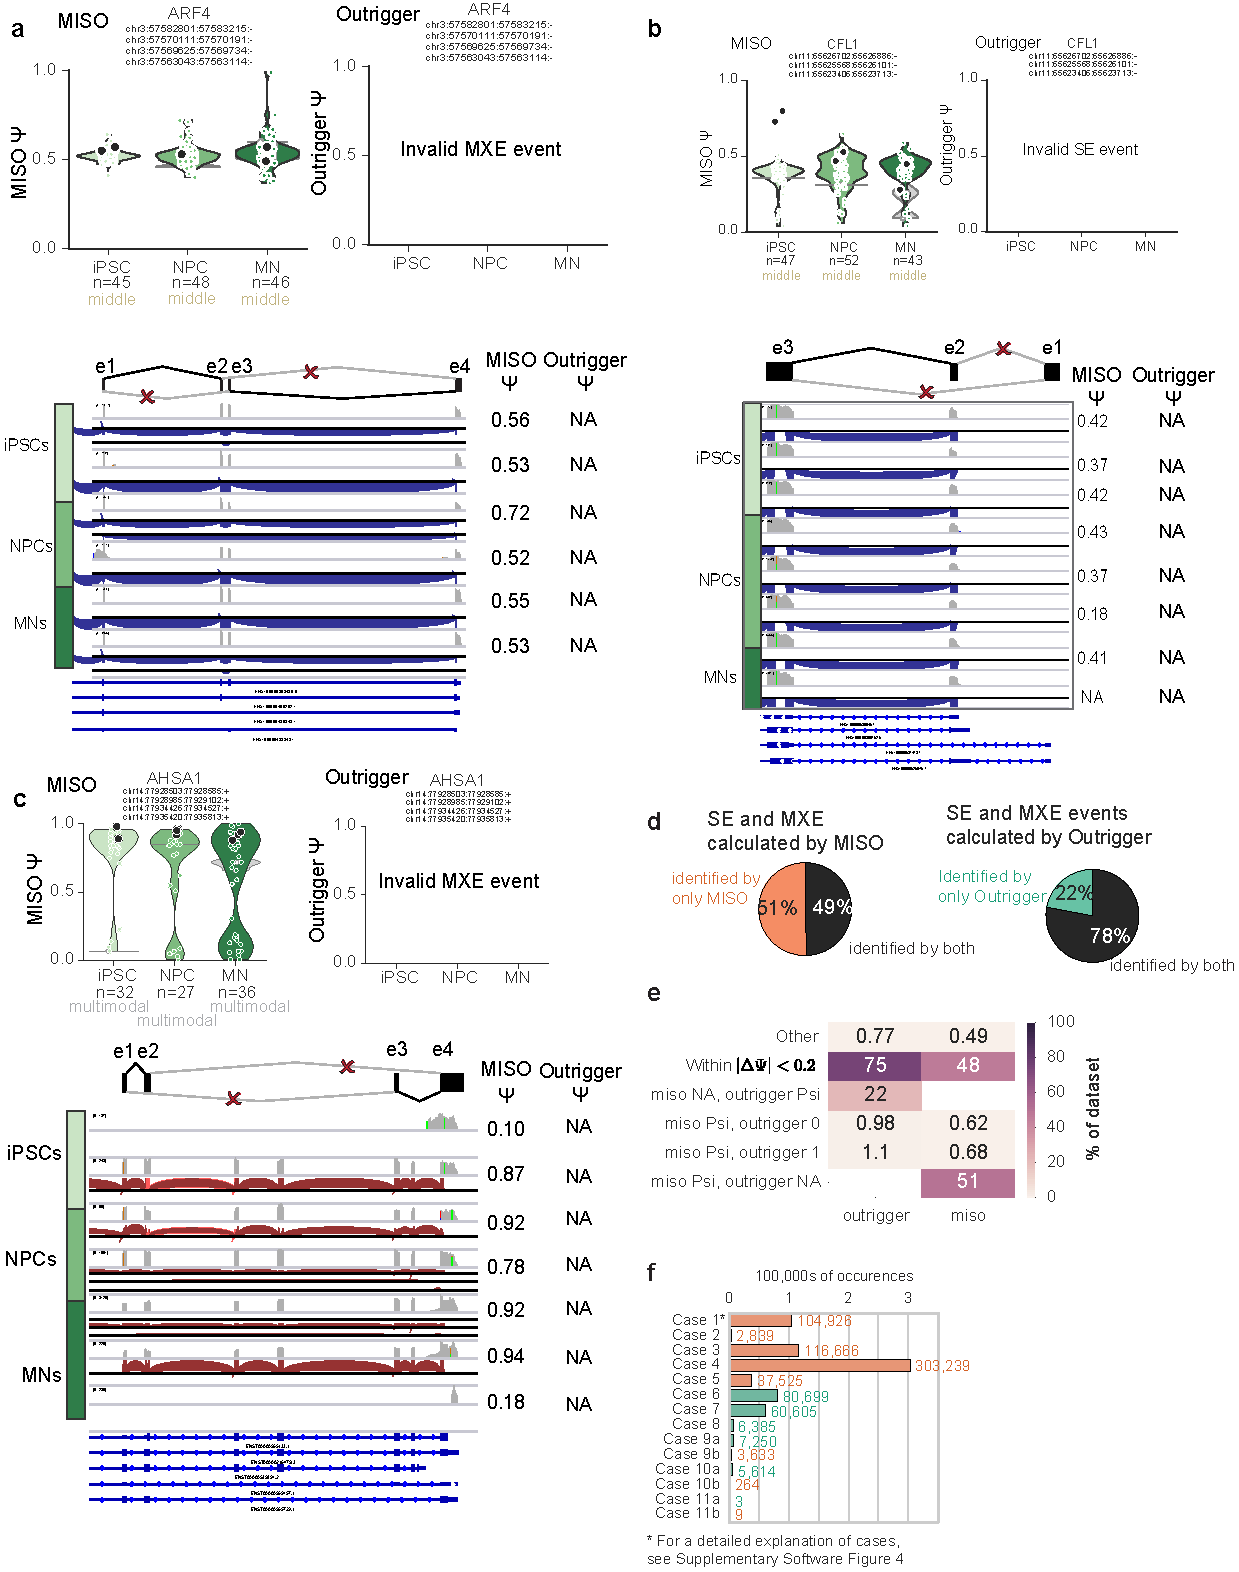
\includegraphics[width=5.8in]{figures/invalid_miso.pdf}
\end{figure}
%and, I'm not sure why, but one of the times I used this code the figure number wasn't augmented for the next figure, so check your figure numbers and if necessary uncomment the following line
%\addtocounter{figure}{1}
\clearpage
% --- END manual facingcaption for MISO fiugre --- %


The majority of the false positives are Case 4, where only one junction has sufficient reads. As MISO counts both junctions to calculate $\Psi$, shown in \textbf{\Cref{fig:miso}b-c}, many of the events are not covered on both sides of the alternative exons, which may suggest the events are not true SE events, but rather alternative first exon events, for instance.

We used MISO's event definitions and found that as many as 50\% of MISO events did not pass the stringent rules of \outrigger, primarily due to the incompatibility with the annotation of SE and MXE and insufficient coverage (\textbf{\Cref{fig:miso}j-l}).


\section{\texttt{anchor}: Modality estimation}
\label{sec:anchor}

\subsection{Algorithm overview}
\paragraph{Model modalities as beta distributions}

% \theoremstyle{definition}
We define \emph{modality} as a distinct type of distributions. Since $\Psi$s are continuous value between $(0, 1)$, distribution of $\Psi$ can be modeled as Beta distribution. The probability density function for the Beta distribution, $\mathrm{Pr}(\alpha, \beta)$ is defined between $(0, 1)$, with parameters $\alpha > 0$ and $\beta > 0$,

\begin{equation}
\mathrm{Pr}(\alpha, \beta) \sim \frac{1}{\mathrm{B}\left(\alpha, \beta\right)}  x^{(\alpha - 1)} \left(1-x\right)^{(\beta-1)},
\end{equation}

where $\mathrm{B}\left(\alpha, \beta\right)$ is the Beta function, defined by $\alpha > 0$ and $\beta > 0$. It may be easier to think about how the $\alpha$ and $\beta$ parameters affect distribution by observing the mean and variance \textbf{\Cref{fig:anchor_parameterization}a}. The beta distributions can be described by four parameterizations: $1 \leq \alpha < \beta$, $\alpha = \beta > 1$, $\alpha > \beta \geq 1$, $\alpha = \beta < 1$ (\textbf{\Cref{fig:anchor_parameterization}b}). Conveniently, these four configurations correspond to the four modalities we are interested in: $1 \leq \alpha < \beta$ corresponds to \emph{excluded}, $\alpha = \beta > 1$ to \emph{middle}, $\alpha > \beta \geq 1$ to \emph{included}, and $\alpha = \beta < 1$ to \emph{bimodal} (\textbf{\Cref{fig:anchor_parameterization}c}). The final \emph{multimodal} modality corresponds to $\alpha = \beta = 1$, which is equivalent to the uniform distribution used as null model.



\paragraph{Model parameterization}
To describe feature distribution as modalities, we parameterized the four parameterizable modalities and used Bayesian model selection to choose the best model to describe the distribution. Python package \texttt{scipy}\cite{Oliphant:2007dm,Millman:2011jv} was used to implement Beta distribution.
For \1 (\0) modality, we fixed $\beta$ ($\alpha$) at 1 and linearly increased $\alpha$ ($\beta$) from $2$ to $20$ (\Cref{fig:anchor_parameterization}d). We chose $2$ as a starting parameter since it is near the $\alpha=\beta=1$ uniform distribution, as we wanted to allow \0 and \1 distributions with noise. For bimodal (middle) modality, we changed $\alpha$ and $\beta$ simultaneously, monotonically decreasing (increasing) the parameters from $\alpha=\frac{1}{12}$, $\beta = \frac{1}{12}$ ($\alpha = 2, \beta = 2$) to $\alpha = \frac{1}{30}, \beta = \frac{1}{30}$ ($\alpha = 20, \beta=20$). The parameters for bimodal start at $\frac{1}{12}$ rather than $\frac{1}{2}$ because starting the parameters from $\frac{1}{2}$ resulted in more false positive ``bimodal'' events, whereas starting the parameters from $\frac{1}{2}$ ensures any density near $0.5$ is downweighted.


The fit of feature distribution is assessed to the four configurations using Bayes Factors, represented by $K$,

\begin{align}
K^{(m)}
&= \frac{P(D | M_1^{(m)})}{P(D | M_0)}\\
&=
\frac{\sum_{i} P(\alpha_i^{(m)}, \beta_i^{(m)} | M_i^{(m)}) P(D | \alpha_i^{(m)}, \beta_i^{(m)}, M_i^{(m)})}
{\sum P(\alpha_0, \beta_0 | M_0) P(D | \alpha_0, \beta_0, M_0)}\\
&=
\frac{\sum_{i} P(\alpha_i^{(m)}, \beta_i^{(m)} | M_i^{(m)}) P(D | \alpha_i^{(m)}, \beta_i^{(m)}, M_i^{(m)})}
{1}\\
&=
\sum_{i} P(\alpha_i^{(m)}, \beta_i^{(m)} | M_i^{(m)}) P(D | \alpha_i^{(m)}, \beta_i^{(m)}, M_i^{(m)})
\end{align}

Where $M_i^{(m)}$ is the model of interest (e.g. $M_i^{(\mathrm{bimodal})}$) and $\alpha_i^{(m)}, \beta_i^{(m)}$ are the corresponding parameters from the parameterization shown in \textbf{\Cref{fig:anchor_parameterization}d}. The null model, $M_0$ is the uniform distribution, where $\alpha_0 = \beta_0 = 1$, and thus $P(D|M_0) = 1$ for all datasets. We use a Bayes Factor cutoff of $K_{\mathrm{cutoff}}$ to indicate the threshold where the model begins to explain the data reasonably well. In practice we set $K_{\mathrm{cutoff}} = 2^{5}$ ($\log_2 K_\mathrm{cutoff} = 5$).

The \0 and \1 modalities vary only one parameter at a time, whereas middle and bimodal modalities vary both $\alpha$ and $\beta$ simoutanously. Models with more parameters are more likely to fit, thus we fit to the one-parameter models first, assessing whether $K > K_{\mathrm{cutoff}}$ for either \0 or \1. No distribution can fit both \0 and \1 modalities, thus it is assigned to the modality with highest $K$. Next, the distribution is fitted to the two-parameter bimodal and middle models, checking if $K > K_{\mathrm{cutoff}}$. If neither modality applies, we assign the modality to \emph{multimodal} (\textbf{2c}).

% --- BEGIN manual facingcaption for anchor_parameterization --- %
\clearpage
\thispagestyle{facingcaption}
\begin{figure}[h]
\captionsetup{labelformat=prev-page}
  \caption[Overview of \anchor\, parameterization of the Beta distribution.]{
  Overview of \anchor\, parameterization of the Beta distribution.\\
\textbf{a.}~Top, equation for the Beta distribution of the random variable $x$ with parameters $\alpha, \beta > 0$. Bottom left, equation for the mean ($\mu$) of the Beta distribution as a function of its parameters. Bottom right, equation for the variance ($\sigma^2$) of the Beta distribution as a function of parameters.\\
\textbf{b.}~Cartoon of valid values of $\alpha$ and $\beta$ parameters of Beta distribution, showing how the space is partitioned by the modalities.\\
\textbf{c.}~Violinplots representing the four ideal modalities, plus the null ``multimodal'' distribution. Each modality is annotated with examples of four cells representing within-cell distributions of included (dark grey) and excluded (light grey) transcripts, and the corresponding parameters of the Beta distribution.\\
\textbf{d.}~Violinplots of 1 million random samples of the family of Beta distributions specified by the $\alpha$ and $\beta$ ($x$ tick labels) parameterization of the four modalities: excluded, bimodal, included, and middle.}
\label{fig:anchor_parameterization}
\end{figure}
\clearpage
\begin{figure}[h]
\ContinuedFloat
\captionsetup{labelformat=empty}
\centering
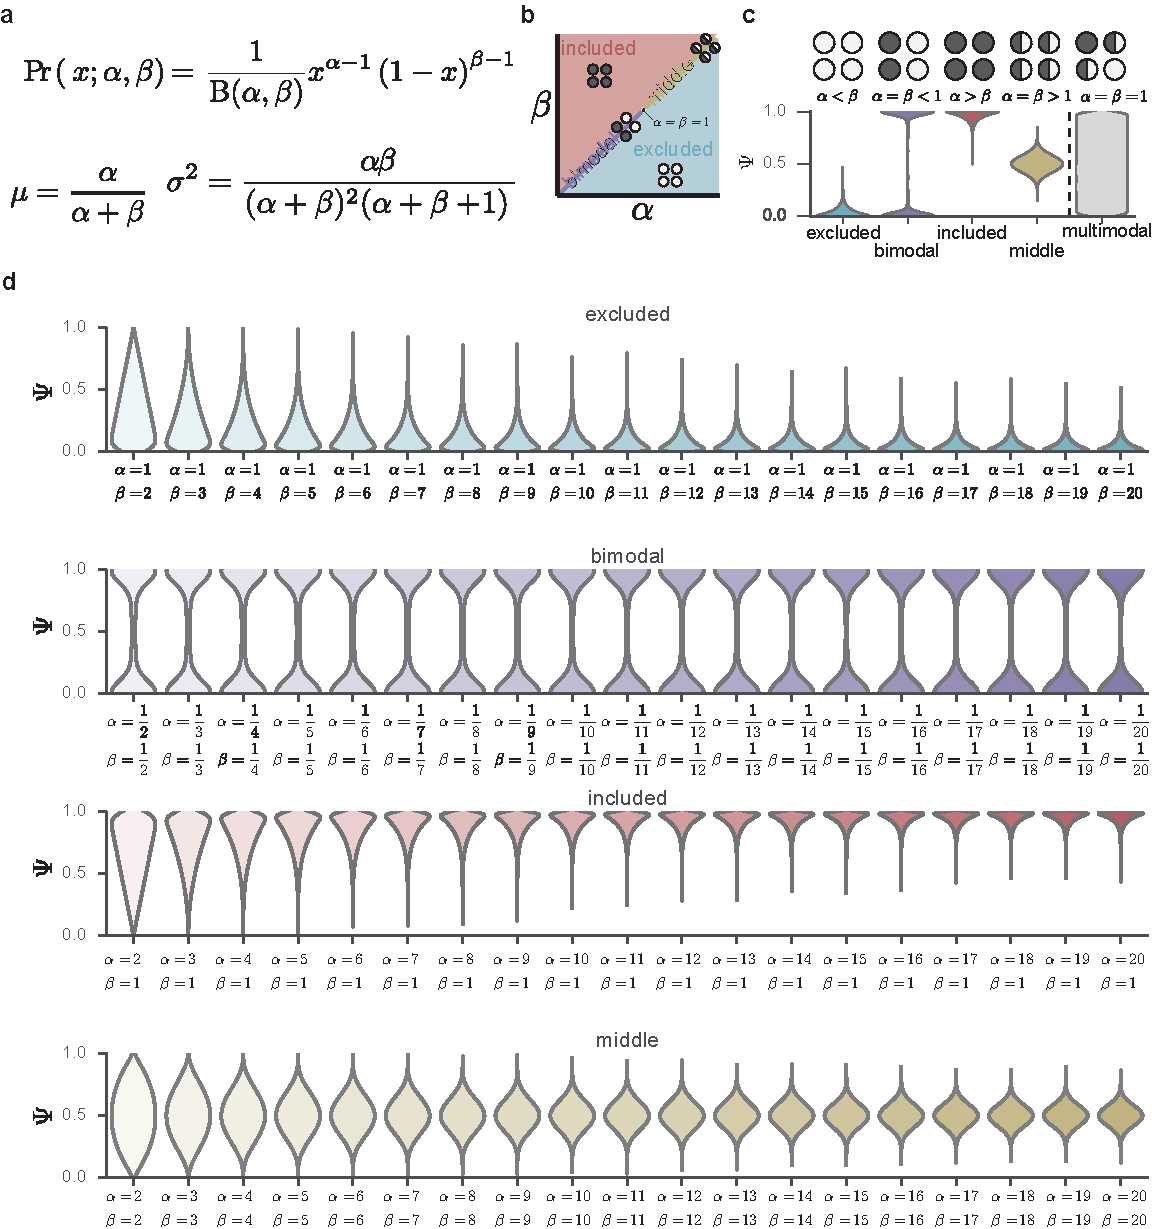
\includegraphics[width=5.8in]{figures/anchor_parameterization}
\end{figure}
%and, I'm not sure why, but one of the times I used this code the figure number wasn't augmented for the next figure, so check your figure numbers and if necessary uncomment the following line
\addtocounter{figure}{1}
\clearpage
% --- END manual facingcaption for anchor_parameterization --- %



As exact $0$ and $1$ are not in the range of the Beta distribution, we implement this model selection by adding a small number ($0.001$) to $0$ and subtracting this small number from $1$. Thus, we approximate the data-derived distribution from the invalid closed interval [0, 1] to the valid open interval of (0, 1).


\subsection{Simulations}

We optimized the algorithm parameters using test datasets and visually inspecting random samples from both the best- and worst-fitting data and ensuring that the even the worst fitting data was still believably categorized as the modality (\textbf{\Cref{fig:anchor_best_worst}}).

\paragraph{Dataset 1: ``Perfect Modalities'' with noise}
\label{sec:anchor_perfect_modalities}

To test the limits of \texttt{anchor}, we simulated perfectly \0, middle, \1, and bimodal distribution, added uniform random noise with 100 iterations, and estimated modality at each noise level with iteration (\textbf{\Cref{fig:anchor_simulations_perfect_modalities}a}). As expected, the most frequently predicted modality was ``multimodal,'' since the dataset was created from randomly added noise (\textbf{\Cref{fig:anchor_simulations_perfect_modalities}b}). The next frequent modality was bimodal, followed by a tie with excluded and included, and the least frequent one is middle modality. We found that these parameterizations can accurately predict modality with up to $35\%$ noise added to the middle modality, $50\%$ noise added to excluded and included modalities, and up to $70\%$ noise added to the bimodal modality(\textbf{\Cref{fig:anchor_simulations_perfect_modalities}d}). By visual inspection of distributions fit best or worst to each modality (\textbf{\Cref{fig:anchor_best_worst}a}), we observed that the bimodal distributions are sufficiently different from other parameterizations, demonstrating the robustness of the algorithm.



% --- BEGIN manual facingcaption for anchor best worst fits --- %
\clearpage
\thispagestyle{facingcaption}
\begin{figure}[h]
\captionsetup{labelformat=prev-page}
  \caption[Best and worst fitting modality data using \anchor.]{
  Best and worst fitting modality data using \anchor.\\
Left, 10 events with largest Bayes Factor, $K$ (best fit) from the assigned modality. Right, 10 events with smallest Bayes Factor, $K$ (worst fit) from their assigned modality. For multimodal, as there is no fit, this simply shows 20 random events.\\
\textbf{a.}~Bayesian \anchor\, method on ``Perfect modalities'' dataset.\\
\textbf{b.}~Bayesian \anchor\, method on ``Maybe bimodals'' dataset.
}
\label{fig:anchor_best_worst}
\end{figure}
\clearpage
\begin{figure}[h]
\ContinuedFloat
\captionsetup{labelformat=empty}
\centering
  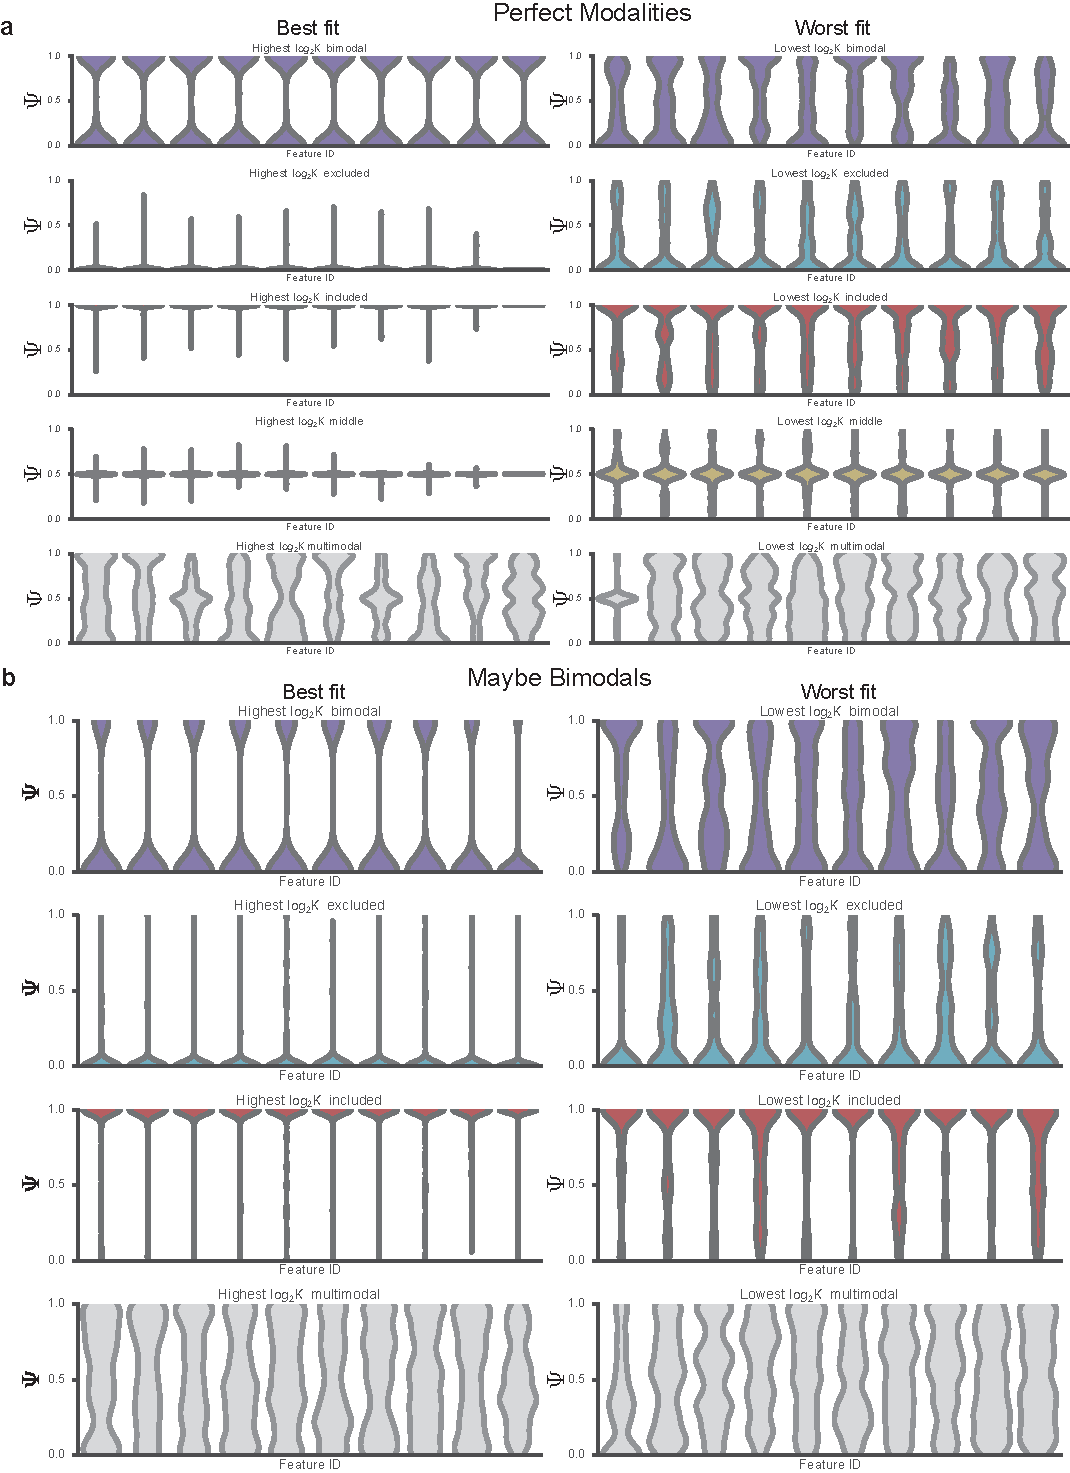
\includegraphics[width=5.8in]{figures/anchor_best_worst}
\end{figure}
%and, I'm not sure why, but one of the times I used this code the figure number wasn't augmented for the next figure, so check your figure numbers and if necessary uncomment the following line
\addtocounter{figure}{1}
\clearpage
% --- END manual facingcaption for anchor best worst fits --- %




% --- BEGIN manual facingcaption for perfect modalities anchor simulations --- %
\clearpage
\thispagestyle{facingcaption}
\begin{figure}[h]
\captionsetup{labelformat=prev-page}
\caption[Simulated ``Perfect Modality'' dataset to test performance of \texttt{anchor}.]{
Simulated dataset to test performance of \texttt{anchor}.\\
\textbf{a.}~Violinplots depicting the creation of simulated modality datasets with increasing noise. The base dataset (\% Noise = 0) consisted of 100 samples of either all zeros (excluded), half zeros and half ones (bimodal), all ones (included), or all $0.5$s (middle), exactly representing the four modalities. Uniform random noise was added in 5\% increments, with 100 iterations at each noise level.
\textbf{b.}~Percentage of events categorized as different modalities by \texttt{anchor} in the randomly generated test datasets, across all noise levels, as illustrated in (\textbf{a}). Number of events for each modality is annotated on top of the barplots. \\
\textbf{c.}~Percentage of events categorized as different modalities by binning in the randomly generated test datasets, across all noise levels, as illustrated in (\textbf{a}). Number of events for each modality is annotated on top of the barplots. \\
\textbf{d-g.}~Specificity of modality estimation. Recapitulation of the original modality as a function of additional noise, using \anchor\, (\textbf{d}), binning (\textbf{e}), Bimodality index (\textbf{f}), and diptest (\textbf{g}) methods. The $x$-axis depicts the percent of uniform random noise added (visualized as a triangle gradient), and the $y$-axis depicts the fraction of times a noisy feature was categorized into each modality. The hue of the line is the modality.
}
\label{fig:anchor_simulations_perfect_modalities}
\end{figure}
\clearpage
\begin{figure}[h]
\ContinuedFloat
\captionsetup{labelformat=empty}
\centering
% \includegraphics[width=5.8in]{sandiego.jpg}
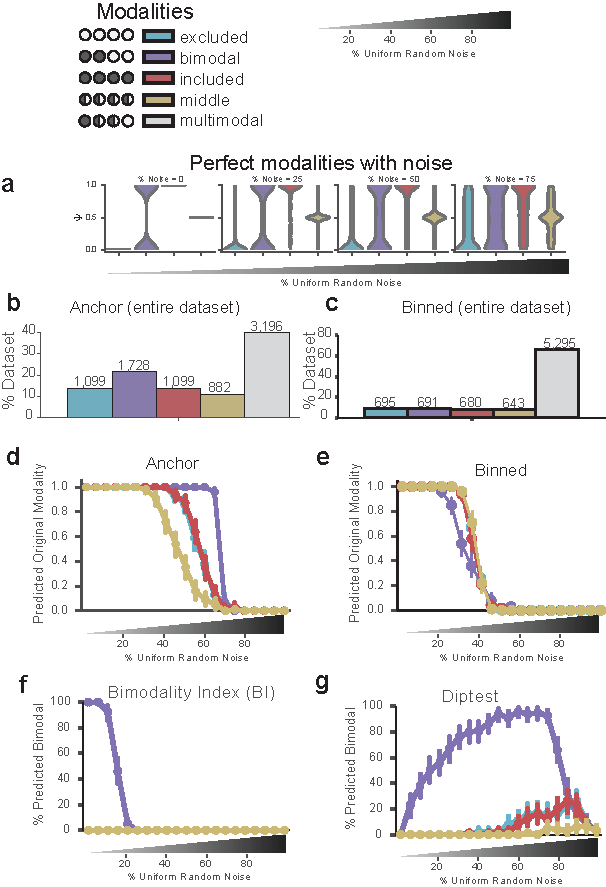
\includegraphics[width=5.8in]{figures/anchor_simulations_perfect_modalities.pdf}
\end{figure}
%and, I'm not sure why, but one of the times I used this code the figure number wasn't augmented for the next figure, so check your figure numbers and if necessary uncomment the following line
\addtocounter{figure}{1}
\clearpage
% --- END manual facingcaption for perfect modalities anchor simulations --- %


\paragraph{Dataset 2: ``Maybe Bimodals'' with noise}
\label{sec:anchor_maybe_bimodals}

To test the proportions of zeros and ones that able to constitute ``bimodal'' distribution, we created another dataset comprised 100 samples of varying amounts of 0s and 1s, and adding random uniform noise (\textbf{~\Cref{fig:anchor_simulations_maybe_bimodals}a}). The primary predicted modality was bimodal, then multimodal, and finally included and excluded (\textbf{Supplementary \Cref{fig:anchor_simulations_maybe_bimodals}b}). No distribution was predicted as the middle modality, indicating the bimodal and middle modalities are drastically different with little chance of mis-assignment. The falloff of correctly predicting bimodality is at adding $70\%$ noise (\textbf{Supplementary \Cref{fig:anchor_simulations_maybe_bimodals}b}), consistent with the previous simulation with ``Perfect Modalities'' dataset (\textbf{\Cref{fig:anchor_simulations_perfect_modalities}d}). We found that bimodality is determing with a 90:10 (10:90) proportion of samples of 0:1 (0:1) (\textbf{Supplementary \Cref{fig:anchor_simulations_maybe_bimodals}d}). Visual inspection of distributions fit best or worst to each modality confirmed the assignment of each modality(\textbf{\Cref{fig:anchor_best_worst}b}).

To summarize, simulation with two different datasets indicates that 1) bimodal modality can tolerate to up to $70\%$ of uniform random noise, and middle modality is least tolerable to noise at only $30\%$, 2) included and excluded modalities are drastically different, so as the middle and bimodal modalities, thus the two step modality assignment procedure (\textbf{Figure 2}) is well-grounded, 3) \anchor is able to determine a bimodal modality with up to 90:10 proportion of zeros and ones.



% --- BEGIN manual facingcaption for maybe bimodals anchor simulations --- %
\clearpage
\thispagestyle{facingcaption}
\begin{figure}[h]
\captionsetup{labelformat=prev-page}
\caption[Simulated ``Maybe Bimodals'' dataset to test performance of \texttt{anchor}.]{
Simulated bimodal dataset to test performance of \texttt{anchor}.\\
\textbf{a.}~Violinplots depicting the creation of the ``Maybe Bimodals'' test set consists of potential bimodal events, each containing 100 samples of only zeros ($\Psi = 0$) and ones ($\Psi = 1$) in every combination, shown here as relative to the number of ones. We added uniform random noise in increasing 5\% levels for 100 iterations at each level. While each combination of 1s and 0s was created, only a subset are shown for brevity -- 1:99, 25:75, 50:50, 75:25, and 99:1 ratios of 1:0 are shown, with added uniform random noise of 0\% (original), 25\%, 50\%, and 75\%.\\
\textbf{b.}~Percentage of events categorized in modalities by \texttt{anchor} in the randomly generated bimodal test datasets, across all noise levels, as illustrated in (\textbf{h}). Number of events for each modality is annotated on top of the barplots. \\
\textbf{c.}~Percentage of events categorized in modalities by binning in the randomly generated bimodal test datasets, across all noise levels, as illustrated in (\textbf{h}). Number of events for each modality is annotated on top of the barplots. \\
\textbf{d-k.}~Accuracy of bimodality prediction, as a function of the noise added to the dataset. \\
\textbf{d-g.}~Specificity of bimodality estimation upon addition of uniform random noise. The $x$-axis shows the percent added uniform random noise (visualized as a triangle gradient), and the $y$-axis indicates the fraction of time features in each noise percentage and proportion of $1:0$ was categorized as bimodal. Overall, all but the very extremes of the $1:0$ proportions were consistently categorized as bimodal until 70\% noise, after which point nearly all events became multimodal. Modality estimations are shown using \anchor\, (\textbf{k}), binning (\textbf{l}), Bimodality Index (\textbf{m}), and Diptest (\textbf{n}).\\
\textbf{h-k.}~Sensitivity of bimodality detection. Percentage of events predicted as bimodal given different proportions of 0s and 1s, and increasing uniform random noise. Events are called as bimodal with approximately 9:1 ratio of 0s and 1s (and vice versa), shown with a dotted line at 10\% ones and 90\% ones. Bottom triangle gradient shows increasing ratio of ones to zeros, i.e. from exclusion to bimodal, to inclusion. Bimodality estimations are shown using \anchor\, (\textbf{o}), binning (\textbf{p}), Bimodality Index (\textbf{q}), and Diptest (\textbf{r}).
}
\label{fig:anchor_simulations_maybe_bimodals}
\end{figure}
\clearpage
\begin{figure}[h]
\ContinuedFloat
\captionsetup{labelformat=empty}
\centering
% \includegraphics[width=5.8in]{sandiego.jpg}
\includegraphics[height=8in]{figures/anchor_simulations_maybe_bimodals.pdf}
\end{figure}
%and, I'm not sure why, but one of the times I used this code the figure number wasn't augmented for the next figure, so check your figure numbers and if necessary uncomment the following line
\addtocounter{figure}{1}
\clearpage
% --- END manual facingcaption for maybe bimodals anchor simulations --- %


\subsection{Comparison to other methods}

\paragraph{Simple binning}
We can compare this to other methods we attempted, such as fixing bins of $[0, 0.3, 0.7, 1]$ and using cutoffs for the densities, which does not account for the continuous nature of the underlying distributions. We found the modality whose binned distribution was the smallest distance (measured by Jensen-Shannon Divergence \cite{Cover:2011vn}) away from each binned event. In both the simulated modalities and simulated bimodal datasets, we found a sharp increase in multimodal distributions and by eye, poorer categorization of the bimodal modality, especially at the decision boundary of low JSD (\textbf{Figures~\cref{fig:anchor_simulations_maybe_bimodals}c, e, j, l, p}).

% \paragraph{Fitting a Beta distribution to individual features}

% or fitting a Beta distribution to each individual feature (which takes a long time) and using cutoffs on the estimated parameters, which is also problematic and error-prone.

\paragraph{Bimodality index}
Another test for bimodality is the Bimodality Index \cite{Wang:2009wm} (BI), which requires estimating each feature as a mixture of Gaussian models. We used the implementation of Generalized Mixture Models in \texttt{scikit-learn} \cite{Pedregosa:2011tv} to estimate two Gaussian distributions for each model, and calculated the BI. For perfect bimodal featues, the value is large, for example, we found that for the zero-noise bimodal event, the $\mathrm{BI}=402$) and was the single bimodality index that was larger than $100$ for any feature (\Cref{fig:anchor_simulations_maybe_bimodals}f, j). This shows that our method is more sensitive to finding bimodal features with the addition of noise, which BI cannot handle.

\paragraph{Hartigan's Dip test}
A commonly used test for unimodality is Hartigan's dip test\cite{Hartigan:1985ca}. If the distribution fails the unimodality test, then it is considered bimodal. To define a cutoff for when the dip statistic becomes reliable, we calculated the dip statistic using a Python implementation of the test, called \texttt{diptest}\cite{Anonymous:zTNIPlgQ}. We used a $p$-value cutoff of $p <0.05$ as our threshold for assigning an event as bimodal. We used the diptest statistic on the two datasets, and found that while the zero-noise bimodal event was not detected as bimodal, adding as small amount of noise \emph{improved} the diptest's detection of bimodal events (\textbf{\Cref{fig:anchor_simulations_maybe_bimodals}g,k}), and the accuracy dropped off at a very high noise level - 90\%. As expected, the excluded, included, and middle modalities weren't detected as bimodal, except at higher noise levels, which we also saw with \anchor.


\section{\texttt{bonvoyage}: Transformation of distributions to \emph{waypoints} and \emph{voyages}}
\label{sec:bonvoyage}

\subsection{Algorithm overview}

The goal of \bonvoyage\, is to be able to summarize the entire distribution of a feature into a single point in space, enabling visualization multiple distributions at a time with intuitive interpretation. To accomplish this, we will transform one-dimensional vectors into two-dimensional space. Specifically, the $x$-axis will represent the \emph{excluded} dimension and the $y$-axis will represent the \emph{included} dimension, and all points will be described as a sum of \0 and \1 components (\textbf{6a}, left). For example, for two distinct cell-types, we can imagine a feature that starts at a \1 modality in the first and changes to a \0 event in the second, or changes from middle to bimodal (\textbf{6a}, right).



\paragraph{Data discretization}
We will use a reduced representation of our splicing data by binning each feature on bins $b$ of size $0.1$, where $b_n$ represents the $n$th bin. We represent the binned splicing matrix with $B_\Psi$, where $B_\Psi[k,j]$ represents the fraction of non-null samples in feature $j$ with $\Psi$ value contained in $b_k$. In practice, we pre-filter the data by using only features for which there are enough samples. In the main text for this paper, we used a minimum of 10 cells.

\paragraph{Dimensionality reduction via non-negative matrix factorization}
Non\hyp{}negative matrix factorization (NMF) is a parts\hyp{}based dimensionality reduction algorithm which results in meaningful, interpretable results \cite{Lee:1999gw}. It is an alternative to other dimensionality reduction methods such as principal- and independent- component analyses (PCA and ICA) because its features are both independent, and non-negative, and thus each feature is composed of a sum of the underlying structure of the data, without pesky negative terms.

Thus, for NMF, we will be reducing $B_\Psi$ as such,

\begin{equation}
B_\Psi \approx W \times H,
\end{equation}

Where $W$ is a (features, $2$)-size matrix of the composition of each feature as a sum of how many samples are excluded and included. We found that in the alternative splicing data, the primary components were the included and excluded values, but in other datasets, this may not be the case. Thus, as the components of NMF are the most prominent features, to ensure reproducibility of the axes across datasets, we seeded the NMF transformation with a matrix that is composed of features that are primarily \0 plus a single \1 feature. We used the Python package \texttt{scikit-learn} \cite{Pedregosa:2011tv} for the Projected Gradient NMF implementation.

We call the projected distributions ``waypoint space,'' and the distance between two points a ``voyage,'' such as the voyage of the MXE event in PKM (\Cref{fig:bonvoyage_overview}c).

% For multiple cell-types, we as we will show in the simulations (the next section, \Cref{subsubsec:bonvoyage_simulations}), we \emph{could} plot all voyages as arrows, but for many at a time, it can be easier to visualize through a hexagonally binned scatterplot, where the $x$-axis is the $\Delta$excluded axis, and the $y$-axis represents the $\Delta$included axis.

\subsection{Simulations}
\label{subsubsec:bonvoyage_simulations}



% The goal of \texttt{bonvoyage} is to identify features which change across groups. As diagrammed in \Cref{fig:example_feature}, the idea is to transform distributions of values into a single point onto \emph{waypoint space}, find the distances between transformed distributions and plot the vectors onto \emph{voyage space}.

\paragraph{Transformation of static distributions}

To demonstrate the ability of\linebreak \texttt{bonvoyage}, we created a simulated dataset which we call ``Maybe Everything'' consisting of every combination of 0s, 1s, and 0.5s (\Cref{fig:bonvoyage_simulations}a-d), essentially incorporating both the ``Perfect Modalities'' (from \Cref{sec:anchor_perfect_modalities}) and ``Maybe Bimodals'' (from \Cref{sec:anchor_maybe_bimodals}) into a single dataset. Again, we added uniform random noise at $5\%$ intervals. We transformed the entire simulated dataset into the \emph{``waypoint''} space.


To identifying features which change in distribution, we calculate the \emph{``voyage''} between them in waypoint space. As a demonstration, we shuffle the simulated data to create two different \emph{in silico} phenotypes. We will use each feature as a \emph{``waypoint''} along the voyage, and calculate total travel distance of each feature between the phenotypes.


A key aspect of the waypoint space is that while changes from exclusion to inclusion are easy to spot by a change in means, the change from a middle to a bimodal is not, and requires a battery of other tests to find. Here, voyage space has a significant advantage as it gives both the magnitude of change and a directly interpretable direction.

% --- BEGIN manual facingcaption for bonvoyage simulations --- %
\clearpage
\thispagestyle{facingcaption}
\begin{figure}[h]
\captionsetup{labelformat=prev-page}
\caption[Visualization capabilities of \bonvoyage\, shown with simulated data.]{Visualization capabilities of \bonvoyage\, shown with simulated data\\
\textbf{a-d.}~Datasets used for testing \bonvoyage. Uniform random noise was added in 5\% intervals to all datasets, up to 95\% noise, for 100 iterations at each noise level.\\
\textbf{a.}~Perfect middle, included, and excluded modalities, with added noise. Only 0\%, 25\%, 50\% and 75\% noise levels are shown for brevity. Top, averaged violinplots for all features at a given level of noise. Bottom, waypoint space of all features at the specified noise level.\\
\textbf{b.}~Maybe middle-included modalities, created with every combination of $0.5$ and $1.0$ values. Only the 0\% noise dataset is shown for brevity. Top, violinplots, bottom, waypoint plots.\\
\textbf{c.}~Maybe excluded-middle modalities, created with every combination of $0.0$ and $0.5$ values. Only the 0\% noise dataset is shown for brevity. Top, violinplots, bottom, waypoint plots.\\
\textbf{d.}~Maybe bimodal modalities, created with every combination of $0$ and $1$ values. Only the 0\% noise dataset is shown for brevity. Top, violinplots, bottom, waypoint plots.\\
\textbf{e.}~Comparison of voyage magnitude and JSD between ``Maybe everything'' data and a shuffled copy to show the entire distribution.
}
\label{fig:bonvoyage_simulations}
\end{figure}
\clearpage
\begin{figure}[h]
\ContinuedFloat
\captionsetup{labelformat=empty}
\centering
% \includegraphics[width=5.8in]{sandiego.jpg}
  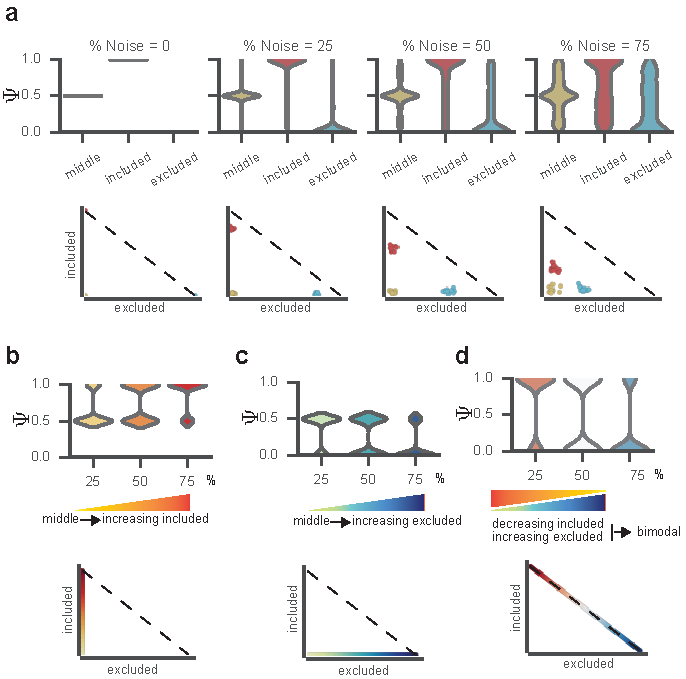
\includegraphics[width=5.8in]{figures/bonvoyage_simulations}
\end{figure}
%and, I'm not sure why, but one of the times I used this code the figure number wasn't augmented for the next figure, so check your figure numbers and if necessary uncomment the following line
\addtocounter{figure}{1}
\clearpage
% --- END manual facingcaption for bonvoyage simulations --- %

\subsection{Comparison to other methods}

As there exist many methods for comparing distributions, we will show that the magnitude of change obtained from \texttt{bonvoyage} is comparable to other metrics for assessing changes in distribution. In particular, we will show the metrics within each modality, and across modalities, compared to Jensen-Shannon Divergence \cite{Cover:2011vn} (JSD) in (\Cref{fig:bonvoyage_simulations}). While JSD is more sensitive to slight changes in distribution (their scatterplots are skewed towards the right), it does not also encode directionality of change. Thus, \texttt{bonvoyage} offers a unique perspective on how to interpret changes in distribution.

\section{Acknowledgements}

Chapter 2, in part, has been accepted for publication as the supplementary material as it may appear in Molecular Cell, 2017, Yan Song$^*$, Olga B Botvinnik$^*$, Michael T Lovci, Boyko Kakaradov, Patrick Liu, Jia L. Xu and Gene W Yeo ($^*$ These authors contributed equally to this work).  The dissertation author was one of the primary investigators and authors of this paper. 
\chapter{Single-cell alternative splicing analysis with Expedition reveals splicing dynamics during neuron differentiation}


\section{Introduction}
Alternative splicing (AS) generates protein diversity in human cells as over 90\% of multi-exon genes are alternatively spliced (Johnson et al., 2003; Pan et al., 2008; Takeda et al., 2010; Wang et al., 2008). Transcriptome profiling by sequencing (RNA-seq) has emerged as a powerful technology to detect and quantify AS in tissue or cell populations (Barbosa-Morais et al., 2012; Merkin et al., 2012; Wang et al., 2008). Neural tissues have especially high levels of alternative splicing, though it is unclear whether it is a result of high levels splicing within each cell or heterogeneity of cells, impeding precise understanding of AS regulation and dynamics. While single-cell technologies (scRNA-seq) can, in principle, address the issue of heterogeneity, and AS variation has been observed in single-cells (Marinov et al., 2014; Shalek et al., 2013; Welch et al., 2016), we still do not know if variable AS events are evolutionarily or biologically distinct from less variable events. Robust computational methods are needed to fully characterize the complexity of AS at the whole transcriptome level in single cells.
Previous studies that investigated AS in single cells were limited to only a few examples (Shalek et al., 2013; Waks et al., 2011) or simply discovered novel splice junctions (Marinov et al., 2014). However, the key challenge in single-cell AS analysis is not only to measure, but to describe variation in AS within a group of single cells, enabling the discovery of differential AS distribution between populations. Most computational tools for AS were developed for bulk RNA-sequencing and were designed for pairwise comparisons to compute relative differences, such as DEXSeq (Anders et al., 2012) and rMATs (Shen et al., 2014). Yet, for single cells, calculating all pairwise comparisons are impractical. Additionally, many algorithms do not consider the compatibility of splicing annotation with the observed data. Algorithms, such as MISO (Katz et al., 2010), utilize probabilistic priors which can assign AS events percent-spliced-in (Psi) values near the prior (Supplementary Software Figure 1), resulting in false positive AS events and also prevent meaningful estimation of splicing variation. Other available methods that reconstruct isoforms or estimate read dispersion (Cufflinks, TIGAR2, WemIQ) (Nariai et al., 2013; Trapnell et al., 2012; Zhang et al., 2015) are not appropriate due to the current low molecular capture rate and uneven transcript coverage in single cell RNA-seq datasets. Thus, the lack of computational tools to describe the distribution of AS limits single cell AS analysis to only a few cells or a few events and prevents us from applying systems biology methods to understand AS complexity on a global scale. Similarly, inability to visualize distribution changes from one cell-type/state to another impedes identification of dynamic AS events subjected to specific regulation.
Three key concepts need to be addressed in single-cell AS analyses: (1) implementation of strict rules to identify AS events and ensure compatibility of the annotation and observed data, (2) description of variation and distribution of AS events and (3) visualization of AS distribution and its dynamics from one cell-type or state to another. Therefore, we developed Expedition, a suite of algorithms integrated in a complete software package. Expedition can identify and quantify AS events in scRNA-seq data (outrigger), categorize splicing modalities (anchor) and visualize modality dynamics (bonvovage). To illustrate its utility we sequenced and analyzed single cells from induced pluripotent stem cells (iPSCs), in vitro differentiated neural progenitor cells (NPCs) and motor neurons (MNs). AS events were quantitated and classified into five distinct modalities. Up to 75\% of AS events exhibit unimodality, where exons are primarily included or excluded with low variance in each cell population. Only ~20\% of AS events are highly varying, composed primarily by bimodal AS events. Interestingly, these bimodal AS events account for essentially all AS events that change modalities during neuronal differentiation, thus representing cell-type specific splicing. Furthermore, we demonstrate that individual bimodal and multimodal events are able to reveal the substructure of a cell population that was undetected by global gene expression analysis. Finally, our study revealed that highly variance AS events exhibit evolutionary and sequence characteristics distinct from unimodal events, illustrating the importance of single-cell analysis of RNA processing.

\section{Results}
\subsection{Identification of alternative splicing events in single cells with \texttt{outrigger}}

To study alternative splicing in a neural differentiation system, human iPSCs were differentiated towards neural progenitor cells (NPCs) and motor neurons (MNs), as supported by immunofluorescence staining and qRT-PCR of known markers (Figure 1a, Supplementary Fig. 1a). We prepared scRNA-seq libraries (Ramskold et al., 2012) which were sequenced to an average depth of 15-25 million, 100 bp paired-end (PE) reads per cell (Supplementary Fig. 1b). Bulk sequencing libraries were also generated from ~1,000 cells. We mapped reads to the hg19 genome using RNA-STAR (Dobin et al., 2013) and estimated gene expression as transcripts per million (TPM) using sailfish (Patro et al., 2014). Genes detected in at least 10 cells were retained and ~4,000-11,000 genes were identified per cell in each population (Supplementary Fig. 1c-d). Downstream analyses were performed on scRNA-seq datasets from 62 iPSCs, 69 NPCs and 60 MNs that satisfied stringent quality control metrics, after excluding outliers detected by k-means clustering (Supplementary Fig. 1e). Lineage-specific transcription factors (POU5F1, PAX6 and ISL1) and RNA binding proteins (LIN28A, MSI1 and RBFOX1) that distinguished each cell-type were observed (Supplementary Fig. 1f). Principal and independent component analysis (PCA and ICA) confirmed that iPSCs, NPCs and MNs were homogenous, yet distinct populations (Supplementary Fig. 1g, h). 

To identify and quantify alternative splicing (AS) events in scRNA-seq, we developed outrigger, an algorithm that uses only junction-spanning scRNA-seq reads to detect and quantify AS. Outrigger then builds a de novo index based on the aligned reads to identify known and novel AS events (Supplementary Fig. 1i, Supplementary Software Figure 2-4). Strict rules were applied to ensure only events with sufficient read coverage, contained valid splice sites, and were compatible with skipped exon (SE) and mutually exclusive exon (MXE) definitions were reported (Supplementary Fig. 1j). Requiring at least 10 reads per junction, outrigger detected ~2,000-10,000 SE and MXE events in each cell. Single iPSCs contained a higher number of AS events (~5,000-10,000) compared to NPCs or MNs (~2,000-6,000) (Supplementary Fig. 1k,l), likely due to higher RNA content in iPSCs. The bulk samples consistently comprised of ~10,000 events, more than most single cells. When an AS event is detected in only a few cells, it may be due to biological variation, aberrant splicing or technical noise. Thus, we retained 13,910 AS events that were detected in at least 10 non-outlier cells in each population within genes that satisfy an expression threshold of TPM>1 (Supplementary Fig. 1m-o). An example of an AS event detected by outrigger is a MXE event of exons 9 (e9) and 10 (e10) in the PKM gene, encoding pyruvate kinase, which is known to be differentially spliced between committed and proliferative tissues (Christofk et al., 2008; Takenaka et al., 1989) (Figure 1b). PKM is highly expressed across the three cell-types, yet individual iPSCs almost exclusively utilizes e10 whereas e9 is the major AS event in MNs, although 20\% (14 out of 60) MNs were observed to possess both isoforms (Figure 1c,d). To verify the differential inclusion of e10 and e9 in iPSCs and MNs, we designed RNA-FISH probes that target constitutive exons of PKM and two probe sets targeting e9 or e10, exclusively. Our RNA-FISH results agreed with outrigger predictions (Figure 1e). Furthermore, ICA based on the Psi value for each AS event within non-differentially expressed genes generalized our findings with PKM splicing. Indeed, single-cell alternative splicing profiles identified by outrigger distinguish the three cell-types (Figure 1f,g), revealing that AS discerns single cell identities, independent of gene expression. 

\subsection{Assignment of single cell alternative splicing events to modalities using anchor}
To categorize the distribution of single cell Psi values, we developed a Bayesian framework, anchor, to designate each AS exon’s distribution into one of five modalities: (1) excluded, where most cells contain the excluded isoform and Psi is close to 0; (2) bimodal, where two subpopulations with either the excluded (Psi near 0) or included isoform (Psi close to 1) can be observed; (3) included, where most cells contain the inclusion isoform (Psi close to 1); (4) middle, where most individual cells have both the inclusion and exclusion isoforms (Psi distribution is centered around 0.5); and (5) multimodal, where the distribution of inclusion and exclusion isoforms does not fit any of the previous categories (Figures 2a,b). Within each cell-type, the Psi distribution for each AS event was modeled using a Beta distribution (Barash et al., 2010). We use a two-step process to assign modality (Figure 2c), a Bayes Factor (K) of fit was first calculated for the one-parameter models, namely included and excluded. If K did not meet the cutoff (), these events are then assessed for their fit to the two-parameter models, namely middle and bimodal. Remaining events were assigned to the multimodal modality. Detection of unimodality was robust up to the addition of ~50\% uniform random noise (Supplementary Fig. 2a-g) and bimodality was detected up to a 9:1 ratio of inclusion to exclusion, and is robust with up to 70\% uniform random noise (Supplementary Fig. 2h-r). Thus, we conclude that anchor is a robust classifier of alternative splicing modalities.

In all three cell-types, exons within the excluded and included modalities account for 25-30\% and 45-50\% of all AS exons analyzed, respectively, indicating that up to 70-80\% of AS events in a given cell-type exhibit unimodality (Figure 2d, Supplementary Fig. 2s), with events largely shared across cell-types (Supplementary Fig. 2t). In comparison, AS events that exhibit bimodality account for up to 20\% of detected AS events, whereas the middle and multimodal modalities account for less than 1\% of AS events. The high-variance bimodal and multimodal events differ the most from bulk samples’ AS estimates with a Δ$\Psi$>0.1 for 40-80\% of the events Supplementary Fig. 2u). Simulations indicate that the observed percentages of unimodal and bimodal AS events are statistically unexpected (random permutations expect 99\% bimodality and ~0\% unimodality; Figure 2e). As we increased the gene expression thresholds, the total number of reliably detected AS events decrease for all modalities. Yet, bimodal events continue to be observed even in the genes with the highest expression (log2TPM > 9, Supplementary Fig. 2v-y), suggesting that sampling biases cannot account for the observation of bimodality. Therefore, our algorithm anchor estimated that most AS events are either included or excluded in single cells, with up to a fifth of events exhibiting bimodality or multimodality, which are undetected in bulk splicing analyses.

\subsection{Splicing modalities exhibit distinct sequence and evolutionary characteristics.}

To investigate whether events in different modalities had distinct properties, we first measured the degree of evolutionary conservation of exon sequences across placental mammals. Expectedly, exon sequences within AS events in the included modality show the highest degree of sequence conservation equivalent to that of constitutive exons, whereas exons in the excluded modality are least conserved (Figure 3a). Bimodal exons exhibit an intermediate level of evolutionary conservation, which is statistically significantly different from excluded and included modalities (q < 10-50, q < 10-100, respectively). However, intronic sequences flanking excluded and bimodal AS are both significantly more conserved than introns flanking included or constitutive exons, a trend that increased along neural differentiation (Figure. 3b and Supplementary Fig. 3a,b). While both excluded and bimodal introns are highly conserved, bimodal introns are more conserved in the 5-20bp window adjacent to the exon-intron junction, whereas conservation for excluded modality decreases in the same region. We also examined the evolutionary history of genes containing bimodal and multimodal exons. Human protein-coding genes have been categorized into 20 phylostrata, with archea as phylostratum 1 (ps1) and human as ps20 (Domazet-Loso and Tautz, 2008). Interestingly, 98 genes harboring multimodal and 1832 genes containing bimodal AS events are more likely found in recent phylostrata in comparison to genes containing excluded, included AS events or all genes containing any AS exon (Figure 3c). Additionally, orthologous exons of 28 bimodal and 3 multimodal AS are more frequently alternatively spliced across mammals (Figure 3d). The exon lengths and the flanking introns of bimodal AS events are significantly longer than those of the included modality and constitutive exons (Figure 3e, Supplementary Fig. 3c). Repetitive elements such as Alu are known to be stochastically exonized(Stower, 2013), and we find Alu elements more enriched in excluded exons, fewer within bimodal exons, and almost absent from AS events in the included modality (Supplementary Fig. 3d). Other features analyzed, including splice site strengths, GC content, showed that bimodal and multimodal exons as intermediate between excluded and included modalities (Supplementary Fig. 3e-i). We conclude that bimodal and multimodal events are enriched for longer flanking introns with higher conservation, present in recently evolved genes, have orthologs in mammals that are also AS events, in agreement we previous findings (Yeo et al., 2005). 

Next, we asked whether there are cis-regulatory elements within flanking intronic sequences. Position weight matrices (PWMs) for motifs recognized by RBPs were obtained from the CISBP motif database (Ray et al., 2013) and transformed into k-mers (Xu and Su, 2010). We defined an intron group as 200 intronic bases upstream or downstream of alternative exons of a specific modality and cell-type. Within each intron group, we calculated Z-scores of k-mer enrichment (Supplementary Fig. 3j,k). By PCA analysis, we found bimodal and included modalities are separated on the first principal component (PC1) and enriched for U-rich and G-rich sequences, respectively (Supplementary Fig. 3l). Curious whether such U-G division is present at the motif level, enriched motifs were identified by calculating a t-statistic between the motif-derived k-mer Z-scores against the Z-scores of all identified k-mers in the same intron group (Supplementary Fig. 3m,n). We then subjected the t-statistics of motif-derived k-mer enrichments in each intron group to PCA (Figure 3f, Supplementary Fig. 3o). Principal component 1 (PC1) explains 72\% of the variance of k-mer enrichment and readily separates the included modality from bimodal modality. Meanwhile, principal component 2 (PC2) distinguishes motifs located upstream or downstream of the alternative exons and account for 8\% of total variance. Consistent with k-mer results, bimodal and included modalities are enriched for U-rich and G-rich motifs, respectively, regardless of the cell-types. Moreover, upstream intronic sequences of included modality are enriched for GC and the downstream counterpart are enriched for GA motifs (Figure 3f, right). This finding suggests that the sequence properties of the introns, together with the trans-factors associated with these motifs distinguish each AS modality, independent of cell-type. Together, our results reveal that exons with highly variant AS events have sequence and evolutionary attributes distinct from other modalities.

Cell-type specific AS are largely comprised of high variance events.
We next asked whether there are AS events that change modalities during the differentiation of iPSCs to NPCs or MNs (Figure 4a, Supplementary Fig. 4a). To our surprise, we find that only ~20\% of AS events shared between pluripotent stem cells and the neuronal derivatives exhibit a change in modality (q < 10-100, hypergeometric test, corrected for multiple hypothesis testing). As these events have a unique modality in each cell-type, they are cell-type specific. Less than a quarter (~18\%) of the AS events detected in two cell-types (iPSCs and NPCs or iPSCs and MNs) exhibited a change in modality (Figure 4b), At least 98\% of these switching events are comprised of bimodal AS events (Figure 4c). As cells transition from iPSCs to NPCs or to MNs, 66\% and 72\% of the unimodal events became bimodal or multimodal, and conversely, 34\% and 27\% of bimodal events switched to a unimodal modality. These “switching” AS events are enriched for GO functional categories, such as ‘protein localization or transportation,’ and ‘RNA processing’ (Supplementary Fig. 4b). Thus, we conclude that bimodal and multimodal AS events likely play an important role in cell-type specificity and are more malleable during differentiation, in contrast to included and excluded events.

Since bimodal and multimodal events are more dynamic, we asked whether they are more likely to preserve protein-coding capacity. For simplicity, the transcripts with excluded and included AS exons are designated as isoform A and isoform B, respectively (Figure 4d). We required that at least one isoform is a GENCODE-annotated coding transcript and utilized hmmscan (Eddy, 1998; Finn et al., 2015) to search Pfam (Bateman et al., 2004; Finn et al., 2016) for protein domain clades (Figure 4e). Both included and excluded modality exons were enriched for the presence of known protein domain clades in their dominant isoform (q < 10-10, hypergeometric test corrected for multiple hypothesis testing). Switching to the other isoform either disrupted the reading frame or the functional protein domain, underscoring the importance of maintaining their dominant isoform. Surprisingly, the bimodal and multimodal AS events appear to balance domain creation, maintenance and disruption between isoforms. In particular, ~65\% of multimodal and ~50\% of bimodal events result in domain maintenance where a functional domain has been exchanged or preserved, in contrast to 15-30\% of excluded and included modalities (Figure 4f). Thus, the highly variant AS events adapt their coding capacity during differentiation.

\subsection{Highly variant AS events can reveal subpopulations invisible to gene expression analysis}

As highly variant bimodal and multimodal AS events appear to be most sensitive to differentiation, we surmised that they can provide an opportunity to identify subpopulations that were otherwise invisible when analyzing gross expression differences in single cell RNA-seq data. To illustrate, SNAP25 (synaptosomal-associated protein 25) is a presynaptic plasma membrane protein of the trans-SNARE complex that mediates synaptic vesicle membrane docking and fusion. Mutually exclusive exons 5a and 5b are characterized as a high variance multimodal event in MNs (Figure 5a-c, Supplementary Fig. 5a). Exon 5b is more included in adult brain (Johansson et al., 2008) which may facilitate faster exocytosis (Nagy et al., 2008). We identified genes that correlated with the Psi values of this event (Spearman correlation |R| > 0.5; Supplementary Fig. 5b). The correlated genes separated the MNs into two clusters that correspond to Psi values of more than 0.5 or less than 0.5 (Figure 5d-g). Excitingly, MNs which included exon 5a (Psi > 0.5) are enriched for genes essential in cytoskeletal reorganization required for axon guidance and dendritic spine formation and maturation, such as KATNAL1, ZMYND10, WASF2 and STX16. They also express genes associated with repression of cell proliferation (Figure 5d, red labels). Thus, MNs utilizing exon 5a are less ‘mature’, may have recently exited cell proliferation and are forming synapses. In contrast, MNs that included exon 5b (Psi <0.5) are enriched with many genes associated with synapse organization and synaptic vesicle trafficking, such as SYNGR3, DCTN1, COPA and PCLO, as well as plasma membrane receptors and cell-cell contact genes such as CELSR2, INADL/PATJ, ATP1B3, and GLRA2. At the same time, these MNs expressed multiple genes associated with intracellular vesicle trafficking (Figure 5d, blue labels), reflecting a more mature neuronal state with active protein transport and vesicle trafficking (Figure 5d). Finally, genes correlating with Psi scores are able to separate the two subgroups in PCA, whereas a complete list of expressed genes from MNs fail to do so (Figure 5f, g). Thus, the variation of the MXE event in SNAP25 reveals substructure in MN populations.

As another example, we observed a SE event from DYNC1I2 (Dynein Cytoplasmic 1 Intermediate Chain 2), which is bimodal in both iPSCs and NPCs (Figure 5h-m, Supplementary Fig. 5c). DYNC1I2 encodes a non-catalytic component of the cytoplasmic dynein 1 complex, which acts as a retrograde microtubule motor to transport organelles and vesicles (Crackower et al., 1999). NPCs were clustered into two groups by genes that correlated with Psi scores of the SE exon (Figure 5j,k). The subgroup with Psi ~1 are enriched for genes associated with a variety of mature neuronal genes, such as ONECUT2, a generic transcription factor of motor neurons and numerous genes related with axon guidance and cytoskeleton reorganization (Figure 5j). This subgroup is also enriched for multiple neuron-specific RNA binding proteins (RBPs), including ELAVL2-4 and SRRM4. On the other hand, the subgroup of NPCs with Psi ~0 is strongly enriched with genes associated with cell division, DNA replication and translation. Again, in contrast to all genes detected in NPCs, only genes correlating with Psi scores reveal the substructures of NPC population in PCA (Figure 5l,m). Thus, the bimodality of this SE event is a sufficient statistic to delineate NPCs into a more proliferative subgroup (Psi ~1) consistent with their progenitor fate and a subgroup (Psi ~0) that appears farther on the trajectory of neuronal fate. 

Lastly, we examined how the multimodal MXE event containing e9 and e10 in PKM distinguishes cell states in MNs. Notably, MNs were partitioned into three subgroups by genes that correlated with the Psi score of this event (Supplementary Fig. 5d-f). The first subgroup is primarily composed of outlier MNs previously characterized by k-means clustering and PCA, which prefers inclusion of exon 9 (Psi < 0.5) and is enriched with genes related to cell proliferation or signaling in progenitor cells (Supplementary Fig. 5d, labeled in light blue). The second subgroup represents MNs also preferring exon 9 (Psi < 0.5), but have lower expression of progenitor genes, and have not expressed neuron-specific genes (Supplementary Fig. 5d, labeled in dark blue). The third subgroup MNs using exon 10 (Psi > 0.5) is highly enriched with neuron-specific genes (Supplementary Fig. 5d, labeled in red) confirming their motor neuron fate. Therefore, a single variance event in PKM provides a sufficient information that unravels distinct cell states (Supplementary Fig. 5f). Many additional examples were found including AS exons in SUGT1, BRD8, MDM4, MEAF6, and RPN2 that demonstrate that high variance AS events extracted from single cells offer an additional layer of information to demarcate cell states that are otherwise hidden in overall gene expression (Supplementary Fig. 5g-o). 

\subsection{Transformation of splicing distributions to “waypoints” reveals dynamic of AS events}

To visualize changes in modalities, we developed bonvoyage, where the distribution of Psi values of each AS event across single cells from a cell-type is first discretized, then reduced via non-negative matrix factorization (NMF) (Figure 6a, left and middle). NMF is a dimensionality reduction algorithm which factorizes data into its components using a parts-based approach (Lee and Seung, 1999). The Psi values are factorized into two components, excluded (x-axis) and included (y-axis), which depict the “waypoint” space (Figure 6a, right). Usage of the waypoint space is illustrated using simulated modality data (Supplementary Fig. 6a-d). Each AS event is depicted as a point in waypoint space, which represents the distribution of Psi scores in single cells (Figure 6b). All the AS events measured in a cell-type were projected into waypoint space, and colored by their corresponding modalities identified previously by anchor (Figure 6c, d). In such a representation, each modality occupies a discrete region in waypoint space. Also, AS events that change their Psi distributions during differentiation undergo “voyages”. To illustrate, exon 9 of PKM is excluded in iPSCs, becomes more included in NPC and is a bimodal exon in MNs. Such a change of modality creates a voyage in waypoint space (Figure 6e). In contrast, projection of this event measured in bulk MNs failed to capture the bimodality. Additionally, MAP4K4 encodes a member of the serine/threonine protein kinase family and inclusion of exon 16 extends MAP4K4’s protein kinase-like domain. This event became progressively more included along MN differentiation, readily observed in a voyage plot, which we independently confirmed by RNA-FISH (Supplementary Fig. 6e-f). Thus, bonvoyage is an effective method to visualize and identify AS events that change across populations.

We next sought to establish a global view of AS changes between cell-types. Focusing on exons with large voyages (Supplementary Fig. 6g), we visualized the voyaging exons using vectors between iPSC and MNs. We regard voyages as complementary to delta Psi (Δ$\Psi$) used in two-sample AS comparisons of bulk RNA-seq data. Consistent with our modality-based analysis (Figure 4a), the majority of the dynamic exons changed from or to the bimodal modality (Figure 6f-g, Supplementary Fig 6h). To evaluate the consequences of voyages on the protein properties of resulting isoforms, we transformed each property into a waypoint-weighted score by multiplying the property of each isoform with its corresponding coordinate in the waypoint space, enabling a more integrated evaluation of protein property based on both isoforms and their distribution in single cells. Among many properties investigated, we found that MNs favor splicing that generates more disordered and basic proteins such as the events in RPS24, and ZNF207/BuGZ (Figure 7a, b). Thus, AS voyages allow for population-based investigation of the protein outcomes of isoform preferences. 

To validate the Psi distributions of bimodal and high-magnitude voyaging AS events during motor neuron differentiation, we designed splicing-sensitive primers to assess exon usage by qPCR at single cell resolution in iPSCs, NPCs and MNs. We observed that ~60\% AS events recapitulated an exon inclusion distribution similar to our findings using scRNA-seq (Figure 7c-f, Supplementary Fig. 7a-n). For example, a SE event that introduces a stop codon and removes three amino acids from C-terminal in RPS24, encoding a ribosomal subunit protein S24, previously reported in different human tissues (Xu and Roufa, 1996). In single cells, this event was partially included in individual iPSCs (middle modality), and became completely included in almost all NPCs and MNs (Figure 7c). These dynamics were confirmed by sc-qPCR (Figure 7d). Also, exon 9 in ZNF207 encoding serine-rich sequences that may affect post-translational modifications, starts as multimodal in iPSCs and becomes more included in MNs (Figure 7e). The dynamics and voyages of these and many other exons were validated by sc-qPCR (Figure 7f, Supplementary Fig. 7a-n). Thus, by enabling comparison of splicing profiles and protein properties, the bonvoyage resource enables visualization of AS dynamics across cell populations.


% Author Contributions
% Y.S., O.B.B. and G.W.Y. conceived and designed experiments; Y.S. and J.L.X. performed the experiments; O.B.B. wrote the Expedition suite and performed computational analysis for the RNA-seq data; P.L., M.T.L. and B.K. assisted with computational analysis; Y.S. performed and analyzed the sc-qPCR and RNA-FISH data; Y.S., O.B.B. and G.W.Y. wrote the manuscript.

% Competing Financial Interests
% The authors declare no competing financial interests.

% Figure Legends

\begin{figure}[h] 
  \centering
  \includegraphics[width=0.5\textwidth]{sandiego}
  \caption[Cell-type specific alternative splicing is an independent feature of cell identity.]{
  Cell-type specific alternative splicing is an independent feature of cell identity.\\
\textbf{a.}~Human iPSCs are directly differentiated into neuron progenitor cells (NPC) or motor neurons (MN) in vitro. Cell identity is verified by immunofluorescence staining. 63 iPSCs (light green), 73 NPCs (medium green) and 70 MNs (dark green) passed QC and were retained for splicing analysis. Bulk samples are independent samples of ~1000 cells.\\
\textbf{b.}~Pyruvate kinase M (PKM) is consistently expressed in iPSCs, NPCs and MNs, shown by log2(TPM+1) in single cells by cell-types.\\
\textbf{c.}~Differential inclusion of a mutually exclusive exon (MXE) alternative splicing (AS) event in PKM is observed in the three cell-types from single cell RNA-seq. top, Schematic of the MXE composed by exon 10 (e10) and exon 9 (e9). bottom, distribution of $\Psi$ for exon 9 in single cells is illustrated by cell-types. $\Psi$ score is estimated by outrigger (see Methods). Each green dot in the violin plots represents one cell. Black dots represent measurements in bulk samples.\\
\textbf{d.}~Coverage track of MXE exons in pyruvate kinase M (PKM) gene. Each row represents a single cell/sample. \\
\textbf{e.}~Preferential inclusion of e10 and e9 in iPSCs and MNs, respectively, were demonstrated in single cells by smRNA-FISH. Probe sets against constitutive exons (green in merge images) and either exon 10 or exon 9 (red in merge images) were designed in PKM gene. Representative smRNA-FISH images for exon 10 (upper) and exon 9 (lower) (left panel). Distribution of normalized exon inclusion is depicted in iPSCs (light blue with dashed outline) and MNs (dark blue with solid outline; right panel). 74 iPSCs and 101 MNs were counted for e10 inclusion; 125 iPSCs and 67 MNs were counted for e9 inclusion. Normalized inclusion fraction is determined by the percentage of exon specific probes co-localized with constitutive probes/constitutive probes, and resulting percentage is normalized by the 95 percentage of the maximal inclusion.\\
\textbf{f-g.}~AS profile is an independent feature of cell-types. 12,685 Non-differentially expressed (non-DE) genes were identified by non-parametric Kruskal-Wallis test with Bonferonni-corrected q-values > 1. \\
\textbf{f.}~ICA on gene expression values of non-DE genes failed to distinguish the three cell-types. \\
\textbf{g.}~ICA on $\Psi$ scores of the AS events residing in non-DE genes, showing AS events are able to group iPSCs, NPCs and MNs, independent of gene expression.
}
  \label{fig:system_overview}
\end{figure}

\begin{figure}[h] 
  \centering
  \includegraphics[width=0.5\textwidth]{sandiego}
  \caption[Assignment of single cell alternative splicing events to modalities using anchor algorithm.]{
  Assignment of single cell alternative splicing events to modalities using anchor algorithm.\\
\textbf{a.}~Schematic of SE and MXE alternative splicing events. Isoform A refers to exclusion of alternative exon (exon 2 in SE and exclusion of exon 2 (black) but inclusion of exon 3 (grey) in MXE), and isoform B refers to inclusion of alternative exon (exon 2 in SE and MXE) of alternative exon. Circles illustrate a single cell containing RNA molecules of a given AS event. Light grey represents isoform A and dark grey represents isoform B. \\
\textbf{b.}~A schematic of the proposed five modalities tested by anchor. Distribution of $\Psi$ for each AS event can be modeled as beta probability distribution parameterized by  and . Modality of excluded ($\Psi$ density concentrated around 0), bimodal ($\Psi$ density concentrated towards 0 and 1), included ($\Psi$ density around 1), middle ($\Psi$ density around 0.5) or multimodal ($\Psi$ density spread out uniformly across 0 to 1). The first four modalities are tested by anchor, and the final multimodal modality represents the null model. \\
\textbf{c.}~Two-step modality assignment process is utilized by anchor. For the $\Psi$ distribution of a given AS event, the Bayes Factor () of fit is first calculated for one-parameter models (only one of  or is parameterized), including included and excluded modalities. If , modality is assigned to the modality with highest . When is not satisfied, an event will be tested in the 2nd step, in which the Bayes Factor () of fit is calculated for two-parameter models (where both  and are parameterized), indicating bimodal and middle modalities. If an event cannot fit at either step, it will be assigned to multimodal modality.  for both steps. Five events from each modality assigned by anchor were randomly selected as examples. 
\textbf{d.}~Composition of AS modalities is similar in iPSCs, NPCs, and MNs. right, zoomed-in panel shows middle and multimodal modality are less than 1\% in the three populations.\\
\textbf{e.}~Composition of modalities of permuted splicing data. Psi scores from all identified AS events in all cells were randomly permuted 1,000 times, then anchor was applied to estimate modalities. Almost 100\% of permuted events are assigned as bimodal. Error bars represents 95\% confidence interval from 1,000 bootstrapped intervals. right, zoomed-in panel shows low percentage of unimodal events in permuted data.
}
  \label{fig:anchor_overview}
\end{figure}

\begin{figure}[h] 
  \centering
  \includegraphics[width=0.5\textwidth]{sandiego}
  \caption[Bimodal AS events exhibit distinct sequence and evolutionary features.]{
  Bimodal AS events exhibit distinct sequence and evolutionary features.\\
All results are shown for iPSCs that have highest number of AS events (12,690). Results are similar in three cell-types, except where indicated. All q-values of significance were derived from multiple hypothesis corrected (Bonferonni) non-parametric Mann-Whitney U test, unless otherwise indicated.\\
\textbf{a.}~Cumulative distributions of the mean Placental Mammal PhastCons score in each modality are shown, with constitutive exons as comparison. AS exons from included modality (red) are as conserved as constitutive exons (black), while excluded exons (blue) are least conserved, followed by bimodal (purple) and multimodal (grey) exons. right, heatmap of pairwise significance scores between each modality or constitutive exons (right panel).\\
\textbf{b.}~Mean Placental Mammal PhastCons scores of flanking intronic regions of exons in excluded (blue) bimodal (purple), multimodal (grey), included (red) modalities, and constitutive (black) exons in all cell-types. bottom, heatmap of base-wise significance of PhastCons scores is presented 0 <  for clarity.\\
\textbf{c.}~Phylostratum scores are summarized for genes harboring AS events in each modality together with genes containing constitutive exons. right, heatmap of pairwise significance scores between each modality or constitutive exons.\\
\textbf{d.}~Alternative splicing events conserved in mammals were extracted from Merkin et al, 2012 (Merkin et al., 2012) and their percentage among each modality is calculated. Hypergeometric test (multiple hypothesis corrected with Bonferonni) indicated q < 10-5 statistical significance. Fraction indicates No. of conserved events in each modality(nominator)/total events in the modality(denominator)\\
\textbf{e.}~Intron lengths summarized in excluded, bimodal, multimodal, included modality together with constitutive exons. top, heatmap of pairwise significance scores between each modality or constitutive exons.\\
\textbf{f.}~Conserved intronic sequences in each modality are enriched with distinct nucleotides. Motifs enriched for each modality are presented by PCA, shown with each circle as a motif and the vectors as component loadings of intron groups. left, Representative motifs are annotated with logos from the CISBP database. right, A simplified illustration of distinct nucleotide enrichment in each intron group. An interactive version of this plot is available at \url{https://plot.ly/~OlgaBotvinnik/32/cisbp-motif-t-test-enrichments-background-phenotype/}
}
  \label{fig:modality_features}
\end{figure}


\begin{figure}[h] 
  \centering
  \includegraphics[width=0.5\textwidth]{sandiego}
  \caption[Dynamic AS events are primarily contributed by highly variant bimodal and multimodal events.]{Dynamic AS events are primarily contributed by highly variant bimodal and multimodal events.\\
\textbf{a.}~AS events change modalities during iPSC to MN transition. A total of 5,675 AS events was identified as common ones in both iPSCs and MNs. The compartmentalization of these common events in five modalities is presented in iPSCs (y-axis) against their corresponding modalities in MNs (x-axis). Gradient of heat map represents the percent of events in the iPSC modality row, annotated with the exact number of events. The diagonal indicates events remained in the same modality. Notably, 88\% of excluded events in iPSCs remained in excluded modality, and 86\% of included events in iPSCs remained as included in MNs. In contrast 52\% of bimodal events in iPSCs switch to either included or excluded modalities in MNs. Multiple hypothesis corrected (Bonferonni) hypergeometric tests were used to calculate significance.\\
\textbf{b.}~During the differentiation from iPSCs to MNs or from iPSCs to NPCs, we found 1,586 (17.6\%) or 1,029 (18.0\%) AS events switched modality, respectively. 
\textbf{c.}~Within the switching events, 99\% events either switched from a bimodal/multimodal state or switched towards a bimodal/multimodal state. Around 1\% of switching events were observed among other types of modality changes.\\
\textbf{d-f.}~AS events in bimodal modality exhibits flexibility in protein coding. 
\textbf{d.}~Schematic of predicted translation changes associated with AS exon inclusion.\\ Exclusion and inclusion of AS exon is termed as Isoform A and Isoform B, respectively. Six categories of coding outcomes are depicted when the isoform switch occurs. Pink, highlights creation of translated proteins or protein domain clades when AS exon is included. Purple, represents maintenance of protein clades with or without change of domain clades. Blue, represents loss of domain clades or disruption of translation when AS exon become included. The square and circle illustrate different Pfam domain clades. The square with dashed outline represents translated protein, possibly containing a Pfam domain clade.\\
\textbf{e.}~The coding outcomes are summarized in the six categories based on all AS events. The percentage of each translation configuration is used as the background distribution for significance calculations in \textbf{f}.\\
\textbf{f.}~AS events in bimodal modality favor protein and domain maintenance. The dominant isoforms in included and excluded modalities favor protein or domain creation and switching to the other isoform results in overwhelming disruption of protein coding. Enrichment is calculated against population average (shown in e) in each category using multiple hypothesis test corrected hypergeometric tests. *: $q< 10^{-10}$  **: $q< 10^{-100}$
}
  \label{fig:dynamic_modalities}
\end{figure}

\begin{figure}[h] 
  \centering
  \includegraphics[width=0.5\textwidth]{sandiego}
  \caption[Bimodal and multimodal AS events reveal subpopulations invisible by gene expression alone.]{Bimodal and multimodal AS events reveal subpopulations invisible by gene expression alone.\\
\textbf{a-g.} SNAP25 alternative splicing reveals a more mature subpopulation in motor neuron population.\\
\textbf{a.}~SNAP25 is primarily expressed in MNs. \\
\textbf{b.}~Usage of alternative exon 5 (a MXE containing exon 5a and exon 5b) in the three populations. Shown is the usage of alternative exon 5a of SNAP25. \\
\textbf{c.}~Summary of exon 5 usage in motor neurons.\\
\textbf{d.}~Preferential usage of exon 5a or exon 5b of SNAP25 in MNs reveals intricate cell states. Genes correlated with the Psi score of this MXE in SNAP25 (above an empirical threshold) were used to cluster all MNs containing this event. Two main subgroups are observed, one with Psi close to 1 (red in the legend bar), the other with Psi close to 0 (blue in the legend bar). Cells with Psi around 0.5 are illustrated with yellow. Black and light grey indicate qualified and outlier MNs based on $k$-means clustering, respectively. Gradient of purple indicates gene expression in $\log_2(\text{TPM}+1)$, with darker being highly expressed. A few representative genes from the two subgroups are highlighted. \\
\textbf{e.}~Examples of representative genes correlating with Psi of this MXE in SNAP25. KATNAL1 and ANAPC16 are more enriched in the cells with $\Psi \approx 1$. DCTN1 and PCLO are more enriched in the cells with $\Psi \approx 0$. X-axis represents the Psi score, and y-axis represent gene expression in $\log_2(\text{TPM}+1)$. Each MN is depicted as a green circle. Solid green line represents simple linear regression line between Psi and the expression of indicated genes. Shaded green represents 95\% confidence interval of the regression.\\
\textbf{f-g.}~Genes correlating with this MXE event distinguish the two subgroups of MNs. Each MN is depicted as a dot in PCA.  Red: cells with $\Psi \approx 1$; blue: $\Psi \approx 0$; yellow: $\Psi \approx 0.5$; X: cells with a Psi assigned as NA.\\
\textbf{f.}~PCA of all expressed genes in MNs failed to separate the two subgroups.\\
\textbf{g.}~Using only the genes correlated with Psi of the MXE in SNAP25, two subgroups are readily separated. Percentage of variance explained are labeled at each PC.\\
\textbf{h-m.}~A bimodal SE event in DYNC1I2 as an example to dissect NPCs into a more proliferating subgroup and a subgroup on the trajectory of neuronal differentiation.\\
\textbf{h.}~Expression of DYNC1I2 in the three populations.\\
\textbf{i.}~Psi distribution of a SE event in DYNC1I2 in the three populations. This event is bimodal in both iPSCs, NPCs and becomes included in MNs.\\
\textbf{j.}~Genes correlating with Psi of this SE event is able to cluster the NPCs into two subgroups. Rows represent the genes and columns represent single cells in NPCs. Genes detected in NPC and correlated with Psi (Spearman $R > 0.5$). Green: NPC. Blue: cells with Psi around 0. Red: cells with Psi around 1. Light Blue to yellow: cells with Psi around 0.5. Black and grey: cells designated as qualified cells versus outlier-cells based on k-means clustering. Representative genes enriched in the two subgroups are highlighted in blue or red. \\
\textbf{k.}~Example genes enriched in the two subgroups of NPCs. ONECUT2 and DCC are more highly expressed in cells with $\Psi \approx 1$; ORC3 and MKI67 are more highly expressed in cells with $\Psi \approx 0$. Psi scores of the SE in DYNC1I2 is plot on x-axis and expression of indicated genes is plotted on y-axis.\\
\textbf{l-m.}~Only genes correlating with Psi are able to separate two subgroups in NPCs, with each NPC depicted as a dot in the PCA. Red: cells with $\Psi \approx 1$; blue: $\Psi \approx 0$; yellow: $\Psi \approx 0.5$; X: cells with a Psi assigned as NA. \\
\textbf{l}.~PCA of all expressed genes in NPCs failed to separate the two subgroups.\\
\textbf{m.}~Genes correlating with Psi are able to segregate the two subgroups by PCA.
}
  \label{fig:hidden_cell_states}
\end{figure}

\begin{figure}[h] 
  \centering
  \includegraphics[width=0.5\textwidth]{sandiego}
  \caption[Bonvoyage visualizes dynamic AS changes.]{Bonvoyage visualizes dynamic AS changes.\\
\textbf{a.}~A schematic to illustrate the transformation of splicing profiles into the two-dimensional waypoint space by bonvoyage. Splicing distribution of each event (A, B, C and D represent 4 different AS events) was discretized into bins (left), factorized by non-negative matrix factorization (NMF) and projected onto 2-dimensional space (middle), such that each data point represents a distribution of alternative splicing. The origin point represents a distribution that all cells have 50\% of inclusion and 50\% exclusion reads observed in scRNA-seq. When the distributions of the same event (either event B or C) are visualized in two different cell-types or states, the dynamic of the event is illustrated by its voyage in the waypoint space (right panel).\\
\textbf{b.}~AS events in iPSCs projected in the waypoint space. The shade of hexagon indicates the number of events. \\
\textbf{c.}~AS events in iPSCs (same as \textbf{b}), colored by the modality estimated by anchor. Each dot represents distribution of one AS event. Note, each modality occupies a distinct region of the waypoint space. Black-outlined circle highlights PKM MXE event.\\
\textbf{d.}~AS events in MNs are colored by their modalities and presented in waypoint space. Black-outlined square highlights PKM MXE event.\\
\textbf{e.}~Dynamics of the MXE event in PKM is illustrated in the waypoint space. Shown is the inclusion of exon 9 of the MXE, which is included in both iPSCs and NPCs and becomes bimodal in MNs.\\
\textbf{f-g.}~Global splicing dynamics between iPSC and MN, aggregated by voyage direction instead of modalities. \\
\textbf{f.}~Number of events originated in iPSC and travel in the indicated directions to land in excluded, bimodal, included, middle, or multimodal modality in MN. \\
\textbf{g.}~Same data as (\textbf{f}), visualized by vectors representing the iPSC (tail) and MN (tip) position of the alternative exon. Color of arrows are coded based on event modalities in iPSCs.
}
  \label{fig:bonvoyage_overview}
\end{figure}

\begin{figure}[h] 
  \centering
  \includegraphics[width=0.5\textwidth]{sandiego}
  \caption[qPCR validation and summary of biological findings.]{qPCR validation and summary of biological findings.\\
\textbf{a-b.}~Waypoint-weighted protein properties changing between iPSC and MN. Significant changes(blue) are identified by a factor of three on Mahalanobis distance relative to all iPSC-MN comparisons.\\
\textbf{a.}~Protein disorder by IUPred, where a score above 0.5 (red dashed line) indicates disorder.\\
\textbf{b.}~Isoelectric point (pI), where the black dashed line indicates $\text{pI}=7$. X-axis, weighted protein property in iPSC and y-axis, weighted protein property in MN. 
\textbf{c-f.}~Distribution of AS inclusion is verified by single cell qRT-PCR (sc-qPCR). Primer sets for inclusion, exclusion and gene expression were designed for each event tested. Percent inclusion measured in sc-qPCR is calculated by $\frac{2^{\text{inclusion Ct}}}{2^{\text{inclusion Ct}} + 2^{\text{exclusion Ct}}}$ (See Methods for more details) in both iPSCs ($n =134$) and MNs ($n = 95$). \\
\textbf{c.}~Percent spliced-in (Psi/$\Psi$) distributions for RPS24 exon 5 measured by single-cell RNA-Seq shown as violinplots (left) and voyages (right).\\
\textbf{d.}~Percent exon inclusion distributions for RPS24 exon 5 measured by single-cell qPCR shown as violinplots (left) and voyages (right).\\
\textbf{e.}~Percent spliced-in (Psi/$\Psi$) distributions for ZNF207 exon 9 measured by single-cell RNA-seq shown as violinplots (left) and voyages (right).\\
\textbf{f.}~Percent exon inclusion distributions for ZNF207 exon 9 measured by single-cell qPCR shown as violinplots (left) and voyages (right).\\
\textbf{g.}~Summary: At single cell resolution, three main categories of modalities can be identified: included, excluded and bimodal. Each modality has unique sequence, coding and evolutionary features. During cell differentiation, majority of unimodal events are static, whereas the highly variance events are dynamic, playing a key role in shaping the transcriptome.
}
  \label{fig:validation_summary}
\end{figure}


\section{Methods}

% For some reason have to add the paragraph indent size here because
% it gets ignored if it's only in the preamble
% \setlength\parindent{24pt}


\subsection{Cell culture and differentiation}

iPSCs were cultured on matrigel coated plated using mTeSR (Stem Cell Technologies) media with mTeSR supplement at $37^\circ$ C incubator with 5\% CO$_{2}$.\par

Neuronal progenitor cells (NPCs) were differentiated from iPSCs. Briefly, iPSCs were cultured in Matrigel coated plates and dislodged by dispase. To form embryonic bodies, the dislodged colonies were cultured in DMEM/F12(invitrogen) with GlutaMax and N2 supplement in non-adhere petri dish. Media were replaced every other day for 7 days. EBs were then plated onto matrigel coated plate to allow rosette formation. Clean rosette were picked manually and maintained in EB media for 7 days and subsequently dissociated with accutase and cultured in NPC media (DMEM/F12, GlutaMax, N2 and B27 with \SI[per-mode=symbol]{2}{\micro\gram\per\micro\liter} FGF) to allow neuron progenitor cell differentiation. NPCs were maintained in NPC media.

Motor neurons were directly differentiated from iPSCs as previous described\cite{Chambers:2009ey}. Briefly, iPSCs were cultured on matrigel coated plates until fully confluent in mTeSR then switch to knock-out serum replacement media (KSR) containing Dorsomorphin(\SI{1}{\micro\Molar}) and SB431542 (\SI{10}{\micro\Molar}). Upon day 4 of differentiation, increasing amounts of N2 media (25\%, 50\%) was added to the KSR. From day 7 of differentiation, \SI{1.5}{\micro\Molar} retinoic acid and \SI{200}{\nano\Molar} Smoothened Agonist (SAG, EMD Millipore) were added to induce patterning. Cells were dissociated on day 17 of differentiation and replated in poly-D-lysine and laminin coated plates. Maturation was performed using BDGF (\SI[per-mode=symbol]{2}{\nano\gram\per\micro\liter}), GDNF (\SI[per-mode=symbol]{2}{\nano\gram\per\micro\liter}), CNTF (\SI[per-mode=symbol]{2}{\nano\gram\per\micro\liter}), ascorbid acid, sonic hedgehog and retinoic acid in N2 and B27 media up until 35 days of differentiation.


\subsection{Single-cell capture and library preparation}

iPSCs, NPCs and MNs were dissociated using Accutase (Stem Cell Biotechnologies) and filtered through \SI{40}{\micro\meter} cell strainers to obtain single cell suspension. Single cells were captured on C1 auto prep platform (Fluidigm, CA) according to manufacturer’s instructions. C1 auto prep chips were visually inspected with a light microscopy at 20X to ensure singularity of captured cells. All non-single cells were discarded from analysis. SMARTer Ultra Low RNA cDNA Synthesis Kit (Clontech) was used to reverse transcribe polyA-tailed RNA. cDNA was amplified using Advantage 2 Polymerase Mix by PCR at \SI{95}{\degreeCelsius} for 1 minutes, followed by 21 cycles of 15 seconds at \SI{95}{\degreeCelsius}, 30 seconds at \SI{65}{\degreeCelsius} and 6 minutes at \SI{68}{\degreeCelsius}, followed by another 10 minutes at \SI{72}{\degreeCelsius} as a final extension. cDNAs were inspected using Agilent Bioanalyzer High Sensitivity DNA chips and quantitated by PicoGreen dsDNA Assay kit (ThermoFisher). cDNAs were diluted to \SI{1}{\nano\gram} to generate libraries using the Nextera XT DNA kit (Illumina, La Jolla, CA). Libraries were multiplexed and sequenced on Illumina HiSeq 2000 to generate 100bp PE reads.

\subsection{RNA-Seq processing}

RNA-seq reads were trimmed using \texttt{cutadapt} v1.8.1 of adapter sequences \texttt{TCGTATGCCGTCTTCTGCTTG}, \texttt{ATCTCGTATGCCGTCTTCTGCTTG}, \texttt{CGACAGGTTCAGAGTTCTACAGTCCGACGATC}, \texttt{GATCGGAAGAGCACACGTCTGAACTCCAGTCAC}, $\left[\text{\texttt{A}}\right]_{50}$, $\left[\text{\texttt{T}}\right]_{50}$, mapped to repetitive elements (RepBase v18.05 \cite{Jurka:2005tp}) using the STAR\cite{Dobin:2013fg} splicing-aware aligner (v2.4.01). Reads that did not map to repetitive elements were then mapped to the human genome (hg19), using GENCODE\cite{Harrow:2012cx} (v19) gene annotations to create the splice junction database. We used the  \texttt{SJ.out.tab} files from STAR to create alternative splicing annotations and calcluate percent spliced-in (see Sec.~\ref{sec:outrigger}). Gene expression was quantified with sailfish\cite{Patro:2014jd} using GENCODE v19 protein-coding and long non-coding RNA annotation, and we then aggregated transcript-level expression to genes.

% \subsection{PCR duplicate removal}

% We removed reads which had exactly the same sequence and alignment location using the command \texttt{rmdup} from the \texttt{samtools} suite\cite{Li:2009kaa}. We then indexed the duplicate-removed .bam files with \texttt{samtools index}.

\subsection{Single-cell expression-level quality control and outlier detection}

We retained genes expressed with TPM $> 1$ in at least 10 cells for a total of 18,594 genes, and filtered out cells which had $<4,000$ expressed genes, which was a natural cutoff in the data. For the three cell types, $n=63$ iPSCs, $n=73$ NPCs, and $n=70$ MNs had enough expressed genes to pass gene expression level quality control.

% \subsection{Outlier detection}

We performed $K$-means clustering with $k=3$ on the gene expression matrix, with 1000 different random initializations. For each cell that clustered into a group that consisted of a majority of a different cell type (e.g. a motor neuron that was clustered in the group with majority NPCs), we called these cells outliers and discarded them from analysis. Overall, for iPSC: 71 were captured, 63 passed  QC,  1 outlier for 62 total; for NPC: $98$ were captured, 73 passed QC, 4 outliers for 69 total; for MN: $93$ were captured,  70 passed QC, 10 outliers for 60 total.

% iPSC: 71 were captured, 64 passed  QC,  1 outlier for 63 total; for NPC: 65 + 33 CVN = 98 captured, 76 passed QC, 3 outliers for 73 total; for MN: 63 + 30 = 93 captured,  79 passed QC, 9 outliers for 70 total.


\subsection{Estimation of alternative splicing}
We used \outrigger\, to create a custom alternative splicing index on the splice junction (\texttt{SJ.out.tab}) files created by STAR, and used GENCODE v19 to define possible exons. This created $40,534$ skipped exon (SE) and $13,217$ mutually exclusive exon (MXE) possible alternative events, and we calculated percent spliced-in (Psi/$\Psi$) with a minimum of 10 junction reads. We then filtered for events that were alternative, not constitutively included or excluded across all cells. Alternative events were defined by, $0 < \Psi < 1$, $\Psi \neq 0, 1$ in at least one cell. Events were then filtered for events that were detected in at least 10 cells of any celltype, resulting in $13,910$ events.

% \subsection{Quality control of AS using split single cell libraries}
% To ensure that variations in alternative splicing detection is not due to technical variation in our experimental procedure, we assessed robustness in estimating AS events from single cells by comparing AS events from paired libraries generated from divided single-cells (\textbf{Supplementary Fig.~\ref{fig:splicing_qc}c}). We observed that 60\% of the $15,000$-$18,000$ estimated AS events from the ``splits'' of each cell overlap, with a statistically significant correlation in the percent-spliced-in (Psi/$\Psi$) values (Spearman correlation $R~1$; $p$-value $~0$, \textbf{Supplementary Fig.~\ref{fig:splicing_qc}d}, top row) for the shared AS events. In contrast, when two libraries from distinct single IPS cells were compared, the correlation was high but lower than for the split cells (Spearman correlation $R=0.9$, $p~0$; \textbf{Supplementary Fig.~\ref{fig:splicing_qc}d}, bottom row). Furthermore, the pooled samples’ expression and splicing was highly correlated (Spearman $R=0.94$ and $R=0.97$, respectively; \textbf{Supplementary Fig.~\ref{fig:splicing_qc}e}, bottom row), but compared to a split cell, the expression and splicing correlations were smaller (Spearman $R=0.71$ and $R=0.932$, respectively; \textbf{Supplementary Fig.~\ref{fig:splicing_qc}e}, top row).

\subsection{Constitutive exons}

We defined constitutive exons as those that did not appear as the alternative exon in any of the splice types (MXE and SE), and had at least 10 reads on both upstream and downstream junctions, in at leat 10 cells per cell type.

\subsection{ICA on constitutively expressed genes and their splicing events}
First, $12,685$ genes were identified as non-DE genes across the three populations using a non-parametric Kruskal-Wallis test with Bonferroni-corrected $p$-value, called $q$, with $q > 10$ as the cutoff. 

Second, AS events were extracted from non-DE genes and their Psi scores are subjected to Independent Component Analysis (ICA). To impute the null values widespread in splicing data, we replaced NAs with an arbitrary number (100) out the of range of Psi values. We did not find that the choice of the arbitrary number affected the ICA results. We then calculated ICA on the imputed matrix.

\subsection{Hierarchical clustering}

We performed hierarchical clustering on samples in Python, using the \texttt{fastcluster}\cite{Mullner:2013bl} package and performing optimal leaf ordering\cite{BarJoseph:2001tr} using the \texttt{polo}\cite{Anonymous:2FB4UNR9} package. All clustering was performed using the Euclidean distance metric with Ward's method\cite{WardJr:2012te}. We visualized using the matplotlib\cite{Anonymous:matplotlib} and seaborn\cite{Anonymous:hWlQiCz3} visualization libraries in Python.

\subsection{Gene Ontology Enrichment}
We calculated Gene Ontology (GO) enrichment by using the Gene Ontology mapping queried to the Entrez gene database using the Python package \texttt{mygene}\cite{Wu:2012bo,Xin:2016fv}. We calculated GO enrichment using only the ``biological process'' category, and corrected for multiple hypothesis testing using Bonferroni correction as performed in the Python package \texttt{goatools}\cite{Tang:2015ub}.

\subsection{Categorization of alternative splicing ``modes''}
We calculated modality using the default parameters of the \anchor\, software (see Sec.~\ref{sec:anchor}) only on splicing events observed in at least 10 cells per cell-type. The performance of anchor was tested extensively using simulated data in comparison to existing bimodality detecting methods.

\subsection{Sequence annotation of alternative isoforms}

We annotated alternative events and their biological features at different levels of the Central Dogma.

\subsubsection{DNA-level}

\paragraph{Evolutionary conservation.} We used units of evolutionary conservation as measured by Placental Mammal PhastCons\cite{Siepel:2005cu} scores calculated previously\cite{Lovci:2013cq} (\textbf{Figure~3a-b}, \textbf{Supplementary Fig.~\ref{fig:modality_features}}). 

For average conservation of exons, we used \texttt{bigWigAverageOverBed}\cite{Kent:2010ff} to calculate the mean conservation (treating bases without annotated conservation as NA) across each exon. For base-wise conservation, we used the HTSeq\cite{Anders:2015gf} Python package to create a memory-mapped \texttt{GenomicArray}, and queried this object with the intronic intervals.


\paragraph{Repetitive element overlap.} We used the Repeat Masker track\cite{Rosenbloom:2015bg} from UCSC's Genome Browser\cite{Kent:2002bwa} and used \texttt{bedtools intersect}\cite{Quinlan:2010kma} to overlap with our exon definitions. We grouped repeats into families defined by the Dfam\cite{Hubley:2016fu} database of repetitive DNA elements (\textbf{Supplementary Fig.~\ref{fig:modality_features}e}). For simplicity of interpretation, we used only repetitive elements that appeared at least 10 times in the excluded modality, as it was the modality with the most repetitive elements.

\paragraph{Gene age (Phylostratum)}

We used the Phylostratum classification of genes as found previously\cite{DomazetLoso:2008ba} (\textbf{Figure~3e}). For each splicing event, we found all overlapping genes in the same genomic locus, and aggregated all genes with at least one event in each modality. Meaning, a gene could appear in multiple modality categories if it had one exon in the included modality and another in the bimodal category.


\paragraph{$k$-mer counting and motif (PWM) enrichment}
We used placental mammal conserved elements as downloaded from UCSC\cite{Rosenbloom:2015bg}, taking only conserved elements upstream and downstream of alternative exons. We used \texttt{kvector}\cite{Anonymous:ug} to count $k$-mers in these conserved elements, and calculated a $Z$-score of $k$-mer enrichment for each intron group defined by cell-type, intron context, and modality (\textbf{Supplementary Fig.~\ref{fig:modality_features}k-l}, \textbf{Figure~3d}). Interested in which $k$-mers were enriched in each modality, we used the total $k$-mer counts in the intron context and celltype, for all modalities, as the background. We then performed principal component analysis using the Python package \texttt{scikit-learn}\cite{Pedregosa:2011tv} on the modality introns (\textbf{Supplementary Fig.~\ref{fig:modality_features}m}). We labeled $k$-mers by the standard color of the majority nucleotide (if there was a tie for the winner, the $k$-mer was assigned grey) whose squared PCA distance was greater than two squared standard deviations from the center, i.e. an ellipse around the origin of the plot. We used the Python package \texttt{adjustText}\cite{Anonymous:tk} to move the text labels away from each other and make them readable.

To find which RNA binding protein motifs were enriched for different modalities, we used version 0.6 of the CISBP-RNA binding database\cite{Ray:2013br} and transformed each position-weight matrix (PWM) into a Boolean vector of $k$-mers that could exactly fit into the PWM, with no mis-matches (\textbf{Supplementary Fig.~\ref{fig:modality_features}n-o}). We ignored psuedocounts by setting all values $\leq 0.1$ to zero. We then used this Boolean matrix to obtain motif $k$-mers and calcluate enrichment using a $t$-test, as compared to all $k$-mers of that intron group. We then performed PCA on the motif $t$-statistics, using the intron groups as features (\textbf{Supplementary Fig.~\ref{fig:modality_features}p}, \textbf{Figure~3d}). We labeled motifs whose squared PCA distance was greater than two squared standard deviations from the center, i.e. an ellipse around the origin of the plot. We used the Python package \texttt{adjustText}\cite{Anonymous:tk} to move the text labels away from each other and make them readable.


\subsubsection{RNA-level}

\paragraph{Consistency of splicing between bulk and single-cells}
To calculate the total difference between the bulk $\Psi$ and single-cell $\Psi$ estimates, for each event, we calculated the average difference between the pooled sample $\Psi$ and every single-cell $\Psi$, much like a sample mean calculation (\textbf{Supplementary Fig.~\ref{fig:modality_features}a}).

\paragraph{Splice site strength}
We used \texttt{bedtools}\cite{Quinlan:2010kma} and \texttt{pybedtools}\cite{Dale:2011cl} to obtain the $5^\prime$ (relative to exon-intron boundary: -20nt into intron and +3nt into exon) and $3^\prime$ (relative to exon-intron boundary: -3 into exon and +6 into intron), and obtained the transcript sequences for these regions. We used MaxEntScan\cite{Yeo:2004fg} to calculate the strength of the alternative exon (exon 2 in both the SE and MXE cases) splice sites (\textbf{Supplementary Fig.~\ref{fig:modality_features}f-g}).

\paragraph{Expression of splicing events}
For finding the gene expression per splicing event, for each event, we used all genes that could map to it. Sometimes multiple genes could map to a single event, as a result of poor annotation, or multiple read-through transcripts. To mitigate this, for each event, we summed all gene expression by the $\log_2(\mathrm{TPM}+1)$ values, and plotted the distribution of expression per modality (\textbf{Supplementary Fig.~\ref{fig:modality_features}h}).

\paragraph{Intron and exon length}
As we used \outrigger\, to calculate splicing, it also output the lengths of the introns and exons for each alternative event, which is what we used (\textbf{Figure~3c} and \textbf{Supplementary Fig.~\ref{fig:modality_features}d}).


\subsubsection{Protein-level}

We are in the process of packaging the splicing event isoform translation and domain scanning code into a package called \texttt{poshsplice}\cite{Anonymous:uj}.

\paragraph{Protein translation}
Using events which had at least one isoform annotated with a CDS in GENCODE v19 ($22,152$ SE and MXE events), we translated the exon trio and duo (SE, included isoform has three exons and and excluded has two) or exon trios (MXE, both included and excluded isoforms contain three exons) to its transcript-annotated reading frame. If these exons participated in transcripts with multiple reading frames, we used all translations.

\paragraph{Domain search} We used the \texttt{hmmscan} command from the HMMer\cite{Finn:2011eg,Eddy:1998ut} software suite (v3.1b1) to search for protein domains matching those in the manually curated Pfam-A database\cite{Finn:2016bf}. We used a domain-independent E-value cutoff of $10^{-5}$. With this raw data, we observed ``domain switching'' between isoforms in instances such as ``Kinase'' to ``Tyrosine Kinase'', when indeed the exact characters of domain name changed, but the overall function didn't. To alleviate this problem, we aggregated domains into clades using Pfam's annotations. We then annotated each individual event with whether only the exclusion or inclusion isoforms had an annotated translation, only one isoform, contained a clade, both contained the same clade, or the clades switched (\textbf{Figure~4d}).

\subsection{Correlation of splicing to expression}
We correlated bimodal and multimodal splicing events to genes with variant expression, defined as two standard deviations away from the mean variance of all genes. We used Spearman correlation to compare splicing profiles to gene expression, and used a threshold of absolute correlation values $|R| > 0.5$ across all samples.

\subsection{Transformation of splicing profiles to 2d space}

We used \bonvoyage\, (see Sec.~\ref{sec:bonvoyage}) to transform one-dimensional splicing profiles into two-dimensional space (\textbf{Figure~6a-c}), using the default parameters. We performed the transformation within cell-type, and required at least 10 cells per splicing event to transform.

\subsection{Waypoint-weighted protein properties}

To obtain protein properties, we used IUPRED\cite{Dosztanyi:2005gq} to calculate protein disorder and the \texttt{ProtParam} module in BioPython\cite{Cock:2009hj} to calculate aromaticity, instability index, molecular weight, secondary structure properties (alpha-helix, beta-sheet, and turns), flexibility, grand average of hydropathy (GRAVY) and isoelectric point.



We summarized isoform protein properties for each phenotype by using the NMF-transformed waypoint space into a weighted average. Using $p_{\text{included}}$ and $p_{\text{excluded}}$ to represent the protein property value (e.g. molecular weight or disordered protein score) of each isoform, and $w_{\text{included}}$ and $w_{\text{excluded}}$ to represent the splicing event's waypoint space position for the included ($y$) and excluded ($x$) axes. We calculated the weighted protein property, $p_w$, within each phenotype, as we did for the modality and waypoint calculation.

\begin{align}
p_w = p_{\text{included}} w_{\text{included}} + p_{\text{excluded}} w_{\text{excluded}}
\end{align}

For properties that had a relative center, e.g. isolectric point which has a neutral value of 7, we subtracted the center value for each protein property, $p_{\text{center}}$ so the multiplication by the waypoint space would amplify the distance from center.

\begin{align}
p_w = p_{\text{center}} + (p_{\text{included}} - p_{\text{center}}) w_{\text{included}} + (p_{\text{excluded}} - p_{\text{center}}) w_{\text{excluded}} 
\end{align}

\subsubsection{Voyaging protein properties}

Interested in which protein properties which changed significantly between cell types, we used Mahalonobis distance\cite{DeMaesschalck:2000hv} ($d_m$), a non-parametric method of finding outliers from distributions. In the two-dimensional case, this means values that are significantly ``off-diagonal'' when comparing two cell types, e.g. iPSC to MN. We used a multiplier of $3d_m$ as the threshold for highly changing protein properties.

\subsection{Single-cell qPCR and primer design}

Single iPSCs and differentiated MNs were captured on C1 auto prep platform (Fluidigm, CA). All non-single cells were discarded from analysis. cDNA from single cells were prepared using the Single-Cell-to-Ct kit (ThermoFisher, USA) and pre-amplified with a pool of primers designed for the splicing events and the expression of corresponding genes. Inclusion and exclusion primers were specifically designed to quantitate inclusion and exclusion of AS exons and expression primers were designed from constitutive exons. All primers were tested for amplification efficiency. High-throughout quantitative PCR was performed on 96.96 Dynamic Arrays on BioMark system (Fluidigm) according to manufacturer’s instructions. Each pre-amplified STA sample was diluted 1:15 for iPSCs and 1:10 for MNs. 3 housekeeping genes (RPL22, RPL27, PGK) and lineage genes (POU5F1, LIN28A, DPPA2, ISL1, MNX1, STMN2, NFEL, DCX) were included. The full list of primers is available in \textbf{Supplementary Table 1}.

\subsection{qPCR data processing}

The log expression of each primer set $g$ was computed as $\log(E_{g,c}) = 25 - \mathrm{Ct}_{(g,c)}$ where $c$ is the cell and $\mathrm{Ct}_{(g,c)}$ is the $\mathrm{Ct}$ value for corresponding primer set. iPSCs were filtered by (RPL22 $>5$, LIN28A $> 8$ and POU5F1 $> 8$) and MNs were filtered by (RPL27 $> 9$, ISL1 $> 2$ and STMN2 $> 5$). A total of 134 single iPSCs and 95 single MNs were retained for further analysis. If $\mathrm{Ct}_{\mathrm{xp},c}  > 25$ ($\mathrm{Ct}$ value for the expression primer), the corresponding $\mathrm{Ct}_{(\mathrm{inc},c)}$ ($\mathrm{Ct}$ value for the inclusion primer) and $\mathrm{Ct}_{(\mathrm{exc},c)}$ ($\mathrm{Ct}$ value for the exclusion primer) were excluded from analysis. Percentage of inclusion is calculated by $\frac{2^{\mathrm{Ct}_{\mathrm{inc}}}}{2^{\mathrm{Ct}_{\mathrm{inc}}} +2^{\mathrm{Ct}_{\mathrm{exc}}}}$. Distribution of percentage of inclusion is plotted by violinplot or decomposed into 2-dimension space \texttt{(nmf(dataset, 2, ``lee''))} and projected into waypoint space in R.

\subsection{RNA fluorescence in situ hybridization (FISH)}

To verify alternative splicing of MXE event composed of exon 9 and 10 in PKM, we designed 3 probe sets (Custom Stellaris\textregistered\, FISH Probes, Biosearch Technologies, Inc., CA) using the Stellaris\textregistered\, RNA FISH Probe Designer available online. One set against constitutive exons of PKM labeled with Quasar 570, two probe sets specifically against exon9 or exon 10, respectively, labeled with Quasar 670. For Exon16 SE event in MAP4K4, one probe set against constitutive exons was designed and labeled with Quasar 570 and another probe set against exon16 was designed and labeled with Quasar 670.

iPSCs and MNs grown on coverslip were fixed with 3.7\% formaldehyde PFA for 10 minutes at room temperature. The probes for constitutive (\SI{1.25}{\micro\Molar}) and alternative exons (\SI{1.25}{\micro\Molar}) were mixed and hybridized to the cells in 10\% deionized formamide for overnight at \SI{37}{\degreeCelsius}, according to manufacturer’s instructions. For MNs, a probe set against ISL1 is designed and labeled with fluorescein to allow the counting of only motor neurons. 

\subsection{RNA-FISH image acquisition and data processing}

Images were acquired on Applied Precision OMX Super Resolution System at the Microscopy Core in the School of Medicine. Specifically, transmission and acquisition time were set at 100\% and 2 minutes for both FISH probes (constitutive and alternative exons). DAPI was acquired at 10\% transmission and 20 second to localize the cells. Sections were taken at \SI{0.125}{\micro\meter} for the diameter of the cells, usually around \numrange[range-phrase = --]{10}{12}\SI{}{\micro\meter}. The resulting stacks of images were deconvoluted on Applied Precision OMX workstation. Foci of RNA molecules were quantified using Volocity 6.3 (PerkinElmer). The raw count files were then processed in R to compute ratio of exon inclusion. To limit non-specific foci, only the foci identified by both inclusion probe and constitutive probe were counted for included exons. Normalized inclusion ratio is calculated by percentage of included probes co-localized with constitutive probes/constitutive probes, and resulting percentage is normalized by 95 percent of the maximal percentage.


\section{Supplementary Notes}

\subsection{Bimodal AS events that partition cell populations}

Another example is a bimodal SE event in SUGT1 gene (MIS12 Kinetochore Complex Assembly Cochaperone), encoding a protein involved in kinetochore function and required for the G1/S and G2/M transition. Though alternative variants have been observed, their functions are largely unknown. By clustering global expression with Psi of this event, we identified two distinct subgroups of cells clustered by their Psi score. Noticeably, the subgroup with <0.5 Psi score, indicating exclusion of the alternative exon, demonstrates consistently high expression of ZEB1 (Zinc Finger E-Box Binding Homeobox 1), a master transcription factor regulating epithelial polarity, and was recently reported to be highly expressed in neuron progenitor cells to control neuronal differentiation by repressing polarity genes. Progenitor cells losing ZEB1 expression are likely to exit proliferation and become polarized\cite{Singh:2016iz}. Additionally, this subgroup is enriched with MMP16, reported to be expressed in less differentiated cells\cite{Astarci:2012bk} and a few genes associated with signaling (TSPAN14, involved in presentation of ADAM10, and YES1, a src family tyrosin kinase). In contrast, the other subgroup utilizing the alternative exon highly expresses ERC2 (ELKS/RAB6-Interacting/CAST Family Member 2), encoding a protein actively involved in presynaptic organization of cytomatrix at the active zone (CAZ) complex and function as regulators of neurotransmitter release\cite{Ko:2006gx}, suggesting this subgroup may be on the path to become nascent neurons. Supporting such a possibility, this subgroup is enriched with genes associated with different aspects of neuronal differentiation, such as TBC1D1 (acts as a GTPase-activating protein for Rab family protein(s) involving in vesicle trafficking), ELOVL4 (Very Long Chain 3-Ketoacyl-CoA Synthase 4), EOGT (EGF Domain Specific O-Linked N-Acetylglucosamine Transferase, modifying Notch receptor), FAM60A (Subunit of the Sin3 deacetylase complex (Sin3/HDAC), repressing components of the TGF-beta signaling pathway). Lastly, the two outlier NPCs (demonstrated sufficient coverage of this event and highlighted in grey) presenting higher inclusion of this alternative exon, are projected more towards MNs on PCA (Supplementary Fig 1g) in comparison to the rest of NPCs. Thus, among the NPCs demonstrating bimodality of this SE event in SUGT1, the subgroup with exclusion Psi appears to be more `progenitor-cell' like, whereas the subgroup with inclusion Psi is likely to be geared toward nascent neurons. 


\begin{figure}[h] 
%   \centering
  \includegraphics[width=0.5\textwidth]{sandiego}
  \caption[Quality control of single cell expression and splicing data.]{Quality control of single cell expression and splicing data.\\
\textbf{a.} RT-qPCR validation of biomarker expression in the bulk populations of iPSCs (light green), NPCs  (medium green), MNs (dark green). Relative expression of the indicated genes were normalized to housekeeping genes RPL27 and PGK. \\
\textbf{b.} Sequencing depth for single cell libraries were depicted in box plots. On average, 10-20 million reads of 100bp length was obtained. \\
% \textbf{c.}~Percent of reads removed by performing \texttt{samtools rmdup} to remove PCR-duplicated reads implied by identical sequence and alignment location.
\textbf{c.} Number of detected genes for single cell libraries shown as boxplots. Approximately 4,000-6,000 genes were detected at $\mathrm{TPM} > 1$ in single cells. \\
\textbf{d.} Number of detected genes compared to the sequencing depth for each sample. $x$-axis, number of reads that mapped uniquely to the genome (fewer than 10 locations), $y$-axis, number of genes with $\mathrm{TPM} > 1$ detected in each sample. Bulk samples are indicated with a black outline and outlier samples are indicated with a grey outline. Left, iPSC samples, middle, NPC samples, right, MN samples.\\
\textbf{e.} Outlier MN cells identified by K-means clustering exhibited a transcriptome resembling NPCs. Unsupervised hierarchical clustering demonstrated that MN outliers are clustered together with NPCs.\\
% \textbf{e.} Barplots of Bonferonni-corrected $p$-value ($q$) Gene ontology enrichment of biological processes in differentially expressed genes between outliers and non-outliers as found by a non-parametric Mann-Whitney U test.\\
\textbf{f.} Expression of lineage-specific transcription factors (left) and RNA binding proteins (right). Specifically, POU5F1/OCT4 and LIN28A are specific to iPSCs, PAX6 and MSI1 are more highly expressed in NPCs, and ISL1 and ELAVL4 are only expressed in MNs. \\
\textbf{g.} PCA of highly variant gene expression. Highly variant is defined as two standard deviations away from mean gene-level variance across all samples.\\
\textbf{h.} ICA on highly variant gene expression. Highly variant is defined as two standard deviations away from mean gene-level variance across all samples.\\
\textbf{i.}~Overview of \outrigger's three steps and associated commands: indexing (\texttt{outrigger index}), validation (\texttt{outrigger validate}) and percent spliced-in (Psi/$\Psi$) calculation (\texttt{outrigger psi}). In the first step of building an index, \outrigger\, considers the entirety of junction reads from the user-input dataset to detect exons \emph{de novo}, adds annotated exons, then searches for alternative exons. In the second, optional, step of validating the detected events, \outrigger\, removes alternative exons with flanking introns lacking consensus splice sites. For the third step of calculating Psi/$\Psi$, \outrigger\, utilizes junction reads together with alternative exons defined in the indexing step and calculates $\Psi$ for each sufficiently covered event. Only junction reads are used to represent inclusion or exclusion reads. SE, Skipped Exon; MXE, Mutually Exclusive Exons.\\
\textbf{j.}~Barplot showing the \outrigger\, cases found across all splicing events and all samples.\\
\textbf{k.}~The number of AS exons (both SE and MXE event types) detected per single cell library. \\
\textbf{l.}~Histograms of number of cells per detected AS exon, in each cell type. Many AS exons were found in only one cell. A minimum of 10 cells per phenotype used, indicated by a dashed red line.\\
\textbf{m.}~Histogram of gene expression across all single cells in iPSC, NPC and MN populations.\\
\textbf{n.}~Expression of genes containing AS exons. 90\% of the detected splicing events reside in transcripts expressed between ~2.5-10 of $\log_2(\mathrm{TPM}+1)$, as indicated by a dashed black line. \\
\textbf{o.} Number of detected AS events compared to the sequencing depth for each sample. $x$-axis, number of reads that mapped uniquely to the genome (fewer than 10 locations), $y$-axis, number of non-NA AS events detected in each sample. Bulk samples are indicated with a black outline and outlier samples are indicated with a grey outline. Left, iPSC samples, middle, NPC samples, right, MN samples.
}
\label{fig:quality_control}
\end{figure}




\begin{figure}[h] 
  \centering
  \includegraphics[width=0.5\textwidth]{sandiego}
  \caption[Simulated datasets to test performance of \texttt{anchor}.]{
  Simulated datasets to test performance of \texttt{anchor}.\\
\textbf{a.}~Violinplots depicting the creation of simulated modality datasets with increasing noise. The base dataset (\% Noise = 0) consisted of 100 samples of either all zeros (excluded), half zeros and half ones (bimodal), all ones (included), or all $0.5$s (middle), exactly representing the four modalities. Uniform random noise was added in 5\% increments, with 100 iterations at each noise level.
\textbf{b.}~Percentage of events categorized as different modalities by \texttt{anchor} in the randomly generated test datasets, across all noise levels, as illustrated in (\textbf{a}). Number of events for each modality is annotated on top of the barplots. \\
\textbf{c.}~Percentage of events categorized as different modalities by binning in the randomly generated test datasets, across all noise levels, as illustrated in (\textbf{a}). Number of events for each modality is annotated on top of the barplots. \\
\textbf{d-g.}~Specificity of modality estimation. Recapitulation of the original modality as a function of additional noise, using \anchor\, (\textbf{d}), binning (\textbf{e}), Bimodality index (\textbf{f}), and diptest (\textbf{g}) methods. The $x$-axis depicts the percent of uniform random noise added (visualized as a triangle gradient), and the $y$-axis depicts the fraction of times a noisy feature was categorized into each modality. The hue of the line is the modality. \\
\textbf{h.}~Violinplots depicting the creation of the ``Maybe Bimodals'' test set consists of potential bimodal events, each containing 100 samples of only zeros ($\Psi = 0$) and ones ($\Psi = 1$) in every combination, shown here as relative to the number of ones. We added uniform random noise in increasing 5\% levels for 100 iterations at each level. While each combination of 1s and 0s was created, only a subset are shown for brevity -- 1:99, 25:75, 50:50, 75:25, and 99:1 ratios of 1:0 are shown, with added uniform random noise of 0\% (original), 25\%, 50\%, and 75\%.\\
\textbf{i.}~Percentage of events categorized in modalities by \texttt{anchor} in the randomly generated bimodal test datasets, across all noise levels, as illustrated in (\textbf{h}). Number of events for each modality is annotated on top of the barplots. \\
\textbf{j.}~Percentage of events categorized in modalities by binning in the randomly generated bimodal test datasets, across all noise levels, as illustrated in (\textbf{h}). Number of events for each modality is annotated on top of the barplots. \\
\textbf{k-r.}~Accuracy of bimodality prediction, as a function of the noise added to the dataset. \\
\textbf{k-n.}~Specificity of bimodality estimation upon addition of uniform random noise. The $x$-axis shows the percent added uniform random noise (visualized as a triangle gradient), and the $y$-axis indicates the fraction of time features in each noise percentage and proportion of $1:0$ was categorized as bimodal. Overall, all but the very extremes of the $1:0$ proportions were consistently categorized as bimodal until 70\% noise, after which point nearly all events became multimodal. Modality estimations are shown using \anchor\, (\textbf{k}), binning (\textbf{l}), Bimodality Index (\textbf{m}), and Diptest (\textbf{n}).\\
\textbf{o-r.}~Sensitivity of bimodality detection. Percentage of events predicted as bimodal given different proportions of 0s and 1s, and increasing uniform random noise. Events are called as bimodal with approximately 9:1 ratio of 0s and 1s (and vice versa), shown with a dotted line at 10\% ones and 90\% ones. Bottom triangle gradient shows increasing ratio of ones to zeros, i.e. from exclusion to bimodal, to inclusion. Bimodality estimations are shown using \anchor\, (\textbf{o}), binning (\textbf{p}), Bimodality Index (\textbf{q}), and Diptest (\textbf{r}).\\
\textbf{s.}~Summary of total number of AS events identifed by \outrigger\, and their modality identified by \anchor\, for each cell type.\\
\textbf{t.}~Venn diagrams of events shared in modalities between cell types. AS events in included and exluded modality are largely shared across the three cell types, but fewer bimodal events are shared across three cell types. Boxed, all AS events, regardless of modality.\\
\textbf{u.}~Percentage of modality AS events inconsistent with pooled estimates, where the mean difference of psi between singles and pooled ($|\Delta\bar{\Psi}|$) is greater than $0.2$.
\textbf{v-y.}~Effect of the expression level per AS event on modality estimation.\\
\textbf{v.}~Number of genes remaining at the expression cutoffs.\\
\textbf{w.}~Number of AS exons at varying expression cutoffs.\\
\textbf{x.}~Percentage of modality estimated at different expression cutoffs (right, zoomed in panel).\\
\textbf{y.}~Number of modality events estimated at different expression cutoffs (right, zoomed in panel).\\
}
\label{fig:anchor}
\end{figure}





\begin{figure}[h] 
  \centering
  \includegraphics[width=0.5\textwidth]{sandiego}
  \caption[Molecular features of each splicing modality.]{
Molecular features of each splicing modality.\\
\textbf{a.}~Flanking intron sequence is more conserved in  bimodal modality. Shown in motor neurons,  intron conservation of bimodal events is slightly higher than excluded AS events.
\textbf{b.}~Barplot of mean placental mammal PhastCons score in introns flanking modality exons, across cell types. Bimodal exons in motor neurons  and NPCs are statistically enriched for higher conservation as compared to iPSCs (Kolmogorov-Smirnov test, Bonferroni-corrected).\\
\textbf{c.}~Significance (top) and boxplots (bottom) of the length of the alternative exons of different modalities. Constitutive exons are statistically enriched for longer exons, compared to excluded modality (Kolmogorov-Smirnov test, Bonferonni-corrected).\\
\textbf{d.}~Heatmap of the number of AS events in each modality overlapping with repetitive elements with AS exons, shown in iPSC. Excluded modality is statistically enriched for overlap ($q < 10^{-50}$, Hypergeometric test).\\
\textbf{e.}~Significance (top) and boxplots (bottom) of the $5^\prime$ splice site scores of the exon, specifically the splice donor site as measured by MaxEntScan. Bimodal and excluded exons have statistically significantly lower splice site scores than included exons (Kolmogorov-Smirnov test, Bonferonni-corrected).\\
\textbf{f.}~Significance (top) and boxplots (bottom) of the $3^\prime$ splice site scores of the exon, specifically the splice acceptor site as measured by MaxEntScan. Bimodal and excluded exons have statistically significantly lower splice site scores than included exons (Kolmogorov-Smirnov test, Bonferonni-corrected).\\
\textbf{g.}~Significance (top) and boxplots (bottom) of the mean expression level of genes ($\log_2(\mathrm{TPM}+1)$, x axis) harboring corresponding AS events in each modality. While events from all five modalities are detected across entire range of gene expression, genes containing bimodal exons are statistically enriched for lower expression (Kolmogorov-Smirnov test, Bonferonni-corrected).\\
\textbf{h.}~Significance (top) and boxplots (bottom) of the GC content of the alternative exons of different modalities. Excluded exons are statistically enriched for higher GC content, compared to included exons (Kolmogorov-Smirnov test, Bonferonni-corrected).\\
\textbf{i.}~Significance (top) and boxplots (bottom) of the number of exons per gene harboring corresponding modalities, measured by the maximum number of genes in any transcript of a gene. Genes containing excluded exons are statistically enriched for fewer exons per gene (Kolmogorov-Smirnov test, Bonferonni-corrected).\\
\textbf{j.}~Overview of defining ``Intron groups'' defined by cell-type, modality, and intron context, and process for obtaining their conserved $k$-mer $Z$-scores.\\
\textbf{k.}~Boxplots of the $Z$-scores of $k$-mer enrichment in the different intron groups, labeled with a colorbar of modality, intron context, and cell-type.\\
\textbf{l.}~PCA on $k$-mer $Z$-scores, with each point as a $k$-mer and the vector components as the introns. $k$-mers with principal comoponent greater than 2.5 standard deviations away from zero were labeled with the sequence, colored by the majority nucleotide. If there was a tie for the majority nucleotide, it was assigned the color grey. An interactive version of this plot can be viewed here: \url{https://plot.ly/~OlgaBotvinnik/20/modality-k-mer-z-scores-background-phenotype/}. Multimodal is not shown because its $k$-mer enrichment has a much larger range than the other modalities and overwhelms the plot.\\
\textbf{m.}~Overview of motif enrichments calculated from intron groups using a $t$-test and their transformation into PCA for visualization.\\
\textbf{n.}~Boxplots of the $t$-statistics of motif enrichment in different intron groups, labeled with colorbars of modality, intron context, and cell-type.\\
\textbf{o.}~PCA on the $t$-statistics of the Motif enrichment, labeled with the motif ID and RPB name from CISBP v0.6. An interactive version of this plot is available at\\\url{https://plot.ly/~OlgaBotvinnik/32/cisbp-motif-t-test-enrichments-background-phenotype/}
}
\label{fig:supp_modality_features}
\end{figure}


\begin{figure}[h] 
  \centering
  \includegraphics[width=0.5\textwidth]{sandiego}
  \caption[Switching AS events are enriched for transcriptome and post-transcriptional regulation GO terms.]{
  Switching AS events are enriched for transcriptome and post-transcriptional regulation GO terms.\\
\textbf{a.}~AS events change modalities during iPSC to NPC transition. A total of 7,962 AS events was identified as common events in both iPSCs and MNs. Notably, $\approx 82\%$ of excluded events in iPSCs remained in excluded modality, and $\approx 84\%$ of included events in iPSCs remained as included in NPCs. In contrast 42\% of bimodal events in iPSCs switch to either included or excluded modalities in NPCs.\\
\textbf{b.}~Of the common events shared by all three populations, the events changing between iPSCs to NPCs (light green) and iPSCs to MNs (dark green). Venn diagram show the overlap between the two sets of switching AS events and GO function terms for each section of switching events.\\
}
\label{fig:switching_events}
\end{figure}


\begin{figure}[h] 
  \centering
  \includegraphics[width=0.5\textwidth]{sandiego}
  \caption[Highly variant AS events reveal intricacies of cell states.]{
Highly variant AS events reveal intricacies of cell states.\\
\textbf{a.}~Read coverage tracks for SNAP25 in MNs. Numbers indicate observed junction reads.\\
\textbf{b.}~Spearman correlation values of a gene's alternative splicing score ($\Psi$) to gene expression values, with a dotted line at the threshold of $R > 0.5$.\\
\textbf{c.}~Tracks from NPCs were shown to illustrate the bimodal inclusion of exon 5. Numbers indicate observed junction reads covering this SE in DYNC1I2.\\
\textbf{d-f.}~A multimodal MXE event in PKM as an example to dissect MNs into three subgroups.\\
\textbf{d.}~Genes correlating with Psi of the MXE event containing exon 9 and exon 10 (Figure 1) is able to cluster the MNs into three subgroups. Subgroup 1, mostly composed of outliers identified by $k$-means clustering (Supplementary Figure 2), contain characteristic genes for progenitors. Subgroup 2 and 3 are enriched for neuronal genes. Rows represent the genes and columns represent single cells in MNs. Genes detected in MNs and correlated with the Psi, using an emipircally-defined threshold of Spearman's $R$ greater than two standard deviations away from the mean permuted correlation values. Psi/$\Psi$ ranged from 0 (blue) to 0.5 (yellow) to 1 (red). Black and grey: cells designated as qualified cells versus outlier-cells based on $k$-means clustering. Representative genes enriched in two of the subgroups are highlighted in blue (high with exon 10 inclusion) or red (high with exon 9 inclusion). \\
\textbf{e.}~Example genes enriched in two of the subgroups of MNs. MAP2 and NRXN1 are more highly expressed in cells with $\Psi \approx 1$; ETV5 and MASTL are more highly expressed in cells with $\Psi \approx 0$. Psi scores of the MXE in PKM is plot on x-axis and $\log_2(\mathrm{TPM}+1)$ of indicated genes is plot on y-axis.\\
\textbf{f.}~Genes correlating with Psi is able to separate the three subgroups in MNs. Left, PCA using all detected genes in MNs. Right, PCA using genes correlating with Psi.\\
\textbf{g-k.} A bimodal SE event in SUGT1 as an example to dissect NPCs into two subgroups.\\
\textbf{g.}~Genes correlating with Psi of the SE event cluster the NPCs into two subgroups. Genes detected in NPCs and correlated with the Psi. Blue: cells with Psi around 0. Red: cells with Psi around 1. Light Blue to yellow: cells with Psi around 0.5. Black and grey: cells designated as qualified cells versus outlier cells based on $k$-means clustering. Representative genes enriched in two of the subgroups are highlighted in blue (high upon exon exclusion) or red (high upon exon inclusion). \\
\textbf{h.}~Expression of SUGT1 in the three populations.\\
\textbf{i.}~Psi distribution of a SE event (lower) in SUGT1 in the three populations. This event is excluded in iPSCs, and bimodal in both NPCs and MNs.\\
\textbf{j.}~Example genes enriched in the two subgroups of NPCs. TBC1D1 and ELOVL4 are more highly expressed in cells with Psi $\approx 1$; MMP16 and TSPAN14 are more highly expressed in cells with Psi ~0. Psi scores of the SE event in SUGT1 is plot on x-axis and $\log_2(\mathrm{TPM}+1)$ of indicated genes is plotted on y-axis.\\
\textbf{k.}~Only genes correlating with Psi is able to separate the two subgroups in NPCs. Left: PCA using all detected genes in NPCs. Right: PCA using genes correlating with Psi.\\
\textbf{l-o.}~PCA using all detected genes in perspective population fail to identify substructures of seemingly homogenous cells (left panel). PCA using gene correlating with each AS events (right panel) is able to identify the delicate substructures of cells.\\
\textbf{l.}~Bimodal SE event in BRD8 distinguishes iPSC substructure.\\
\textbf{m.}~Bimodal SE event in MDM4 distinguishes NPC substructure.\\
\textbf{n.}~Bimodal SE event in MEAF6 distinguishes NPC substructure.\\
\textbf{o.}~Bimodal SE event in RPN2 distinguishes MN substructure.\\
}
\label{fig:bimodal_correlations}
\end{figure}



\begin{figure}[h] 
  \centering
  \includegraphics[width=0.5\textwidth]{sandiego}
  \caption[Overview of \bonvoyage.]{Overview of \bonvoyage.\\
\textbf{a-d.}~Datasets used for testing \bonvoyage. Uniform random noise was added in 5\% intervals to all datasets, up to 95\% noise, for 100 iterations at each noise level.\\
\textbf{a.}~Perfect middle, included, and excluded modalities, with added noise. Only 0\%, 25\%, 50\% and 75\% noise levels are shown for brevity. Top, averaged violinplots for all features at a given level of noise. Bottom, waypoint space of all features at the specified noise level.\\
\textbf{b.}~Maybe middle-included modalities, created with every combination of $0.5$ and $1.0$ values. Only the 0\% noise dataset is shown for brevity. Top, violinplots, bottom, waypoint plots.\\
\textbf{c.}~Maybe excluded-middle modalities, created with every combination of $0.0$ and $0.5$ values. Only the 0\% noise dataset is shown for brevity. Top, violinplots, bottom, waypoint plots.\\
\textbf{d.}~Maybe bimodal modalities, created with every combination of $0$ and $1$ values. Only the 0\% noise dataset is shown for brevity. Top, violinplots, bottom, waypoint plots.\\
\textbf{e-f.}~Validation of a SE event in MAP4K4 by smRNA-FISH. \\
\textbf{e.}~MAP4K4 smRNA-FISH. Left, probe sets are designed for constitutive exons and alternative exon 16. Exon 16 is excluded in iPSCs ($n = 113$, light purple with dashed line) and become more included in MNs ($n = 68$, dark purple with solid outline. Middle, quantitation of normalized inclusion of exon 16. Arrows point out foci overlapped for both constitutive and exon 16 probes. Normalized inclusion ratio is calculated by percentage of e16 probes co-localized with constitutive probes/constitutive probes, and resulting percentage is normalized by 95 percentage of the maximal percentage. \\
\textbf{f.}~MAP4K4 single-cell RNA-Seq. Left, violinplots percent spliced-in inclusion values, and right, waypoint space of exon 16.\\
\textbf{g.}~Magnitude of change in waypoint space (voyages) from iPSC to NPC, and iPSC to MN, with a cutoff shown as a black dashed line at 0.2.\\
\textbf{h.}~Global splicing dynamics between iPSC and MN modalities, visualized as vectors from iPSC to MN  in waypoint space. Underlying data is the same as \textbf{Figure 4a}. Color of arrows are coded based on event modalities in MNs.
}
\label{fig:bonvoyage}
\end{figure}




\begin{figure}[h] 
  \centering
  \includegraphics[width=0.5\textwidth]{sandiego}
  \caption[Validation of alternative splicing events by sc-qPCR.]{
  Validation of alternative splicing events by sc-qPCR.\\
\textbf{a-g.} Distribution of alternative exon inclusion by single-cell RNA-Seq for indicated events in EWSR1~(\textbf{a}), DYNC1I2~(\textbf{b}), CLTC/CLCT2~(\textbf{c}), EIF5~(\textbf{d}), THYN1~(\textbf{e}), RBPJ~(\textbf{f}), and EIF4A2~(\textbf{g}), shown in violin plots (left) and in waypoint plots (right). Percent spliced-in (Psi/$\Psi$) is calculated based on single cell RNA-seq data, illustrated in green. Black dots indicate bulk samples (~1,000 cells) for each cell type.\\
\textbf{h-n.} Distribution of percentage of inclusion by single-cell qPCR of indicated events EWSR1~(\textbf{h}), DYNC1I2~(\textbf{i}), CLTC/CLCT2~(\textbf{j}), EIF5~(\textbf{k}), THYN1~(\textbf{l}), RBPJ~(\textbf{m}), and EIF4A2~(\textbf{n}), based on single cell qPCR shown in violin plot (left) and waypoint plot (right), illustrated in blue.
}
\label{fig:validation}
\end{figure}



\section{Discussion}
We developed the Expedition software suite to address key aspects of AS analysis from single-cell RNA-seq data. The Expedition suite consists of three packages that integrate the detection and quantification of AS events (outrigger) with the assignment of modalities (anchor), and a method for visualization of changes in modality (bonvoyage). As an application, Expedition was used to analyze AS in single cells from three homogenous cell-types, specifically human pluripotent stem cells, neural progenitors and motor neurons. 

Many studies have performed RNA sequencing from bulk samples to measure AS, where the “relative” inclusion (Δ$\Psi$) of alternative exons in a comparison (e.g. treatment versus control or between tissues) is the primary metric used. However, Δ$\Psi$ comparison across all single cells are impractical. Thus, robust estimation of Psi is required to assess the distribution of Psi amongst a population of single cells. It is also important that Psi values reflect the actual biological phenomenon, such that a Psi value of 0.5 indicates that 50\% of transcripts include the alternative exon while the other 50\% exclude it. Thus, using Psi of 0.5 as a prior in probabilistic models and assessing the confidence of estimates by resampling data (Katz et al., 2010) is not appropriate in single cell splicing analysis as it does not eliminate cases where the observed data and annotation are incompatible (examples shown in Supplementary Software Fig. 1). In contrast, outrigger identifies splicing events by constructing de novo splicing annotation based on only junction-spanning reads, reconstructs the exon trio (quartet) for SE (MXE) events using graph traversal, and quantifies Psi. Outrigger also applies user-defined rules that ensure compatibility and sufficient read coverage of the AS events. 

Anchor enables the robust classification of AS exons into five modalities (included, middle, excluded, bimodal and multimodal). Anchor characterizes AS events by their distribution and variation at the population level using a Bayesian approach, instead of estimating the noise or cell-to-cell variation of AS events (Marinov et al., 2014).  The representation of modalities in all three cell-types is remarkably consistent: ~30\% excluded, ~50\% included and ~20\% bimodal modalities, with small contributions from middle and multimodal modalities, indicating that AS is largely unimodal at the single-cell level. The ability to categorize AS distribution and variation into modalities allowed us to identify distinct sequence and evolutionary features for the three major modalities (summarized in Figure 7g). While high variance bimodal and multimodal AS events exhibit some features intermediate between included and excluded modalities, other features suggest that these AS events reflect an evolutionarily important class of exons distinct from included and excluded. High variance events contain more highly conserved and longer flanking intronic sequences. The conserved flanking intronic sequences contain cis-motifs enriched for U or UA nucleotides, in contrast to the G rich sequence in included modality. G-rich sequences have been shown to create G-quadruplexes that increase efficiency of splicing (Marcel et al., 2011; Ribeiro et al., 2015; Zizza et al., 2016), and thus the lack of G-rich sequences in bimodal may promote their flexibility to be regulated by trans-factors. Interestingly, high variance AS events are also enriched for genes present in more recently evolved phylostrata. This enrichment is concomitant with a peak of gene emergence associated with the evolution of multicellularity, shortly before the Cambrian explosion (Domazet-Loso and Tautz, 2008). At the same time, orthologous exons of the human bimodal AS events detected in our cells are also more frequently regulated as AS across other mammalian lineages (Merkin et al., 2012). 

Lastly, a distinct property of multimodal AS exons is their preference to maintain protein translatability, possibly with a different function, between the two isoforms. It appears that multimodal exons provide cells flexibility to increase protein diversity without severely compromising protein-coding capacity. This is in contrast to the exons within the included or excluded modalities that tend to create or disrupt reading frames. While it is currently unknown whether these multimodal AS events are a consequence of selective allelic expression or splicing, our evidence suggests that the creation and preservation of bimodal AS exons is required to build a flexible repertoire of protein variants to efficiently cope with evolutionary or environmental changes. Moreover, we illustrate that high variance AS events reveals cellular states invisible to gene expression analysis alone, emphasizing the need to analyze AS at the single cell level. Our findings in single cells that high variance AS events are primary determinants of cell-type-specific splicing is reminiscent of findings that the cell-type- or state-specific master regulators are more likely to be variable in either gene expression (Shalek et al., 2013; Shalek et al., 2014) or epigenetic control (Buenrostro et al., 2015).
In summary, our study provides a technological framework to deconvolute the complexity of AS at a single cell level. Prospectively, Expedition can be applied to other increasingly popular data types represented by distributions of continuous variables (including but not limited to RNA-editing, nucleotide modifications such as psuedo-uridine and N6-methyl adenosine, alternative polyadenylation sites, and polyA tail lengths), providing advanced analysis to categorize, and describe these molecular features at single-cell resolution. 

\section{Acknowledgements}
The authors would like to thank members of the Yeo lab for critical reading of the manuscript.  This work was supported by grants from the National Institute of Health (HG004659, NS075449, AI095277, MH107369 and HD085902), the California Institute of Regenerative Medicine (RB3-05009, RB4-06045) and the Brain Research Foundation (BRFSG-2014-14) to G.W.Y. G.W.Y. is an Alfred P. Sloan Research Fellow. O.B.B is a National Defense Science and Engineering Graduate Fellow and a NumFOCUS John Hunter Technology Fellow. We thank Jennifer Santini for technical support from Microscopy Core in the School of Medicine at UC San Diego (NS047101).
%
% Of course, if you prefer, you can just start with
%   \chapter{My First Chapter Name}
% and start typing away.  
% \chapter{Just a Test}
% This is only a test.
% \section{A section}
% Lorem ipsum dolor sit amet, consectetuer adipiscing elit. Nulla odio
% sem, bibendum ut, aliquam ac, facilisis id, tellus. Nam posuere pede
% sit amet ipsum. Etiam dolor. In sodales eros quis pede.  Quisque sed
% nulla et ligula vulputate lacinia. In venenatis, ligula id semper
% feugiat, ligula odio adipiscing libero, eget mollis nunc erat id orci.
% Nullam ante dolor, rutrum eget, vestibulum euismod, pulvinar at, nibh.
% In sapien. Quisque ut arcu. Suspendisse potenti. Cras consequat cursus
% nulla.

% \subsection{A Figure Example}
% \label{ssec:figure_example}

% This subsection shows a sample figure.

% \begin{figure}[h] 
%   \centering
%   \includegraphics[width=0.5\textwidth]{sandiego}
%   \caption[Short figure caption (must be \protect{$< 4$} lines in the list of figures)]{A picture of San Diego.  Note that figures must be on their own line (no neighboring text) and captions must be single-spaced and appear \protect\textit{below} the figure.  Captions can be as long as you want, but if they are longer than 4 lines in the list of figures, you must provide a short figure caption.\index{SanDiego}} 
%   \label{fig:sandiego}
% \end{figure}

% \subsection{A Table Example}

% While in Section \ref{ssec:figure_example} Figure \ref{fig:sandiego} we had a majestic figure, here we provide a crazy table example.


% %%%% TABLE 1 %%%%
% \vspace{0.25in}
% \begin{table}[!ht]
% \caption[Short figure caption (must be \protect{$< 4$} lines in the list of tables)]{A table of when I get hungry.  Note that tables must be on their own line (no neighboring text) and captions must be single-spaced and appear \protect\textit{above} the table.  Captions can be as long as you want, but if they are longer than 4 lines in the list of figures, you must provide a short figure caption.}

% \vspace{-0.25in}
% \begin{center}
% \begin{tabular}{|p{1in}|p{2in}|p{3in}|}

% \hline
% Time of day & Hunger Level & Preferred Food \\

% \hline
% 8am & high & IHOP (French Toast) \\

% \hline
% noon & medium & Croutons (Tomato Basil Soup \& Granny Smith Chicken Salad) \\

% \hline
% 5pm & high & Bombay Coast (Saag Paneer) or Hi Thai (Pad See Ew) \\

% \hline
% 8pm & medium & Yogurt World (froyo!) \\

% \hline
% \end{tabular}
% \end{center}
% \label{tab:analysis3}
% \end{table}



% %% APPENDIX
% \appendix
% \chapter{Final notes}
% What to do about things \cite{Martin_1983}.  What did he say \cite{Rilling_Insel_1999}.
%   Remove me in case of abdominal pain.



%% END MATTER
% \printindex %% Uncomment to display the index
% \nocite{}  %% Put any references that you want to include in the bib 
%               but haven't cited in the braces.
\bibliographystyle{alpha}  %% This is just my personal favorite style. 
%                              There are many others.
%\setlength{\bibleftmargin}{0.25in}  % indent each item
%\setlength{\bibindent}{-\bibleftmargin}  % unindent the first line
%\def\baselinestretch{1.0}  % force single spacing
%\setlength{\bibitemsep}{0.16in}  % add extra space between items
\bibliography{template}  %% This looks for the bibliography in template.bib 
%                          which should be formatted as a bibtex file.
%                          and needs to be separately compiled into a bbl file.
\end{document}

